% !TEX encoding = UTF-8
% !TEX TS-program = pdflatex
% !TEX root = ../Tesi.tex
% !TEX spellcheck = en-EN

%************************************************
\chapter{Artificial Neural Network Generalization}
\label{cap:anntraining}
%************************************************

\section{Principal Component Analysis (PCA) Results}
\label{sec:pcaanalysis}

We evaluated the linear relationship between the microscopic and the
macroscopic parameters in the training simulations with Matlab Principal
Component Analysis.
The results can be seen in Table \ref{tab:06inputRelationshipTable}.
Sliding friction (\acs{mus}), rolling friction (\acs{mur}) and particle density (\acs{rhop})
had the greatest influence on, respectively, the coefficient of pre-shear
(\acs{mupsh}), the angle of repose  (\acs{AoR}) and the bulk density (\acs{rhob}). Notably, \acs{rhop}
was not used as a training parameter for \acs{AoR} bulk behaviour. \\
In fact, we can see how each relationship is below the 100\% necessary to claim
a direct linear correlation.
Thus, we demonstrated that we need more precise statistical tools to investigate
the relationships and generalize the results.

\begin{table}[h]
\centering
\scalebox{1.0}{
\begin{tabular}{c|cccccccc}
\hline
          & $\mu_s$ & $\mu_r$ & $COR$ & $\rho_p$ & $\mu_{sh}$ & $\mu_{psh}$ & $\rho_{b}$ & $AOR$ \\
          \hline
    $\mu_s$ & 100.00 & 0.55  & 0.04  & 0.00  & 3.84  & 87.26 & 8.39  & 49.48 \\
    $\mu_r$ & 0.55  & 100.00 & 0.15  & 0.00  & 58.92 & 33.70 & 3.10  & 60.20 \\
    $COR$ & 0.04  & 0.15  & 100.00 & 0.00  & 15.52 & 0.57  & 1.71  & 0.00 \\
    $\rho_p$ & 0.00  & 0.00  & 0.00  & 100.00 & 4.98  & 5.71  & 99.00 & 0.00 \\
    $\mu_{sh}$ & 3.84  & 58.92 & 15.52 & 4.98  & 100.00 & 26.03 & 9.52  & 0.00 \\
    $\mu_{psh}$ & \textbf{87.26} & 33.70 & 0.57  & 5.71  & 26.03 & 100.00 & 4.33 
    & 0.00
    \\
    $\rho_{b}$ & 8.39  & 3.10  & 1.71  & \textbf{99.00} & 9.52  & 4.33  & 100.00
    & 0.00 \\
    $AOR$ & 49.48 & \textbf{60.20} & 0.00  & 0.00  & 0.00  & 0.00  & 0.00  &
    100.00 \\
    
\hline
\end{tabular}}
\caption{Values of linear relationship between considered variables multiplied
for 100}
\label{tab:06inputRelationshipTable}
\end{table}

\section{Regression statistic training concept}
\label{sec:regressiontrainingconcept}

\begin{figure}[!htb]
\centering
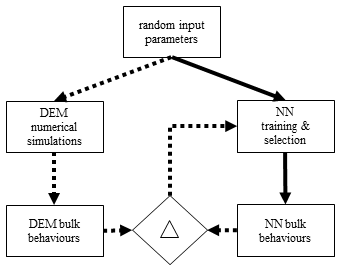
\includegraphics[width=.50\columnwidth]{images/127anntraining}
\caption[ANN training]{ANN training.}
\label{fig:127anntraining}
\end{figure}

Initially, as shown in Fig. \ref{fig:019methodology} in the training phase
(dashed lines) \acs{DEM} simulations are performed
with random initial input parameters.
The behaviours obtained are used to train the following regression models:
\begin{itemize}
  \item{Bayesian linear,}
  \item{Gaussian non linear,}
  \item{Artificial Neural Network (\acs{ANN}).}
\end{itemize}
For all the three models training consists in a loop that continues until the
difference between the outputs of each model and its samples is below the
limit ($\Delta$) (see Chapter \ref{cap:ann} for more details).\\
Thus, we were able to use the \acs{DEM} parameter combinations and their
corresponding bulk values to train the models.
Especially, we divided the samples in three pools: the first, with 70\% of the
samples, as \textit{training set}, the second, with 15\% of the samples, as
\textit{generalization set}, for early stopping, and the third, as \textit{test
set}, as suggested by Haykin (2009). The assignment of each sample to each pool
was random.

\subsection{ANN training concept specifications}
\label{subsec:anntrainingconceptspecifications}

The training of an \acs{ANN} consists in defining the weights and the biases for
each of its neuron.
We first defined the typology of Artificial Neural Networks (\acs{ANNs}) we used and
the input we fed them, see Benvenuti et al. \cite{RefWorks:205}.
Our \acs{ANNs} have three different layers: the input layer has a number of neurons
equal to the number of different inputs of the network, see Fig.
\ref{fig:018nnscheme}, with the scheme of how the Multilayer Perceptron \acs{ANN} ($MLPNN$) derives one
bulk-behaviour-dependent variable from the mutually independent simulation variables.
The hidden (or central) layer's number of neurons was to be investigated. 
The output layer contains one neuron for the output.
The transfer function for the neurons of the central layer is the tangential
sigmoid, while the neuron of the output layer use the linear transfer
function.\\
\begin{figure}[!htb]
\centering
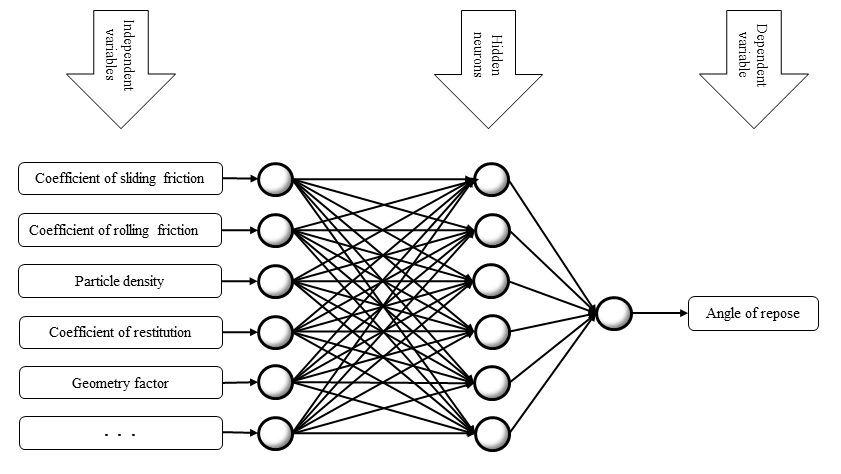
\includegraphics[width=.96\columnwidth]{images/129NN22}
\caption[ANN Scheme]{Artificial Neural Network (\acs{ANN}) Scheme. Regressors
are show in the left-hand side of the image. An example of a response is shown
in the right-hand side of the image.}
\label{fig:018nnscheme}
\end{figure}
We started with all the \acs{DEM} parameter combinations and their corresponding
numerical \acs{mupsh} from the \textit{training set} to create 36 \acs{ANNs} that
differed in their numbers of neurons in the hidden layer (between five to forty neurons).
The \textit{generalization set} was used to speed the training. 
We then determined the coefficient of determination (\acs{r2}), 
\begin{equation}
R^2 = \frac {SSR}{SST} = 1 - \frac {SSE}{SST} .
 \label{eq:rsquare}
\end{equation}

between the
$bulk-macro$ behaviours in the output of the \acs{ANN} and the \textit{test
set} simulations, which were not correlated with the remaining 70\% used for the
training.
Thus, we could select for \acs{mupsh} the \acs{ANN} with the maximum \acs{r2}, 
again as suggested by Vaferi et al. \cite{RefWorks:150}, and we noted its number
of neurons.
We repeated the same \acs{ANN} creation steps for \acs{mush}, \acs{rhob}
and \acs{AoR}, obtaining one trained \acs{ANN} for each bulk value. \\

\subsection{Sinter fine ANN training}
\label{subsec:sinterfineanntraining}

As said, we started with the sinter fine.
The first bulk value \acs{ANN} trained was the \acs{mupsh}, where we achieved a
$\acs{r2} = 0.96$ for an \acs{ANN} with twenty neurons, a consistent agreement
between the \acs{DEM} and the \acs{ANN} values, which demonstrates the accurate predictive power of
the \acs{ANN}, compared to the other two methods.
Increasing the number of neurons did not improve the \acs{r2}; it even started to
oscillate with higher numbers of neurons.
The weights and biases, which represent the trained network, can be be found in
Table \ref{tab:34weightsoriginalsinterfinesct}.
In Fig. \ref{fig:022regression} the corresponding plot for the \acs{ANN} with the maximum \acs{r2} is shown. 
Each circle represents one of the 546 simulations. \\
We subsequently obtained the optimal number of neurons for all
\acs{ANNs}. Table \ref{tab:35weightssinterfineaor} shows the weights for the
\acs{AoR}.\\

\begin{figure}[!h] 
\centering 
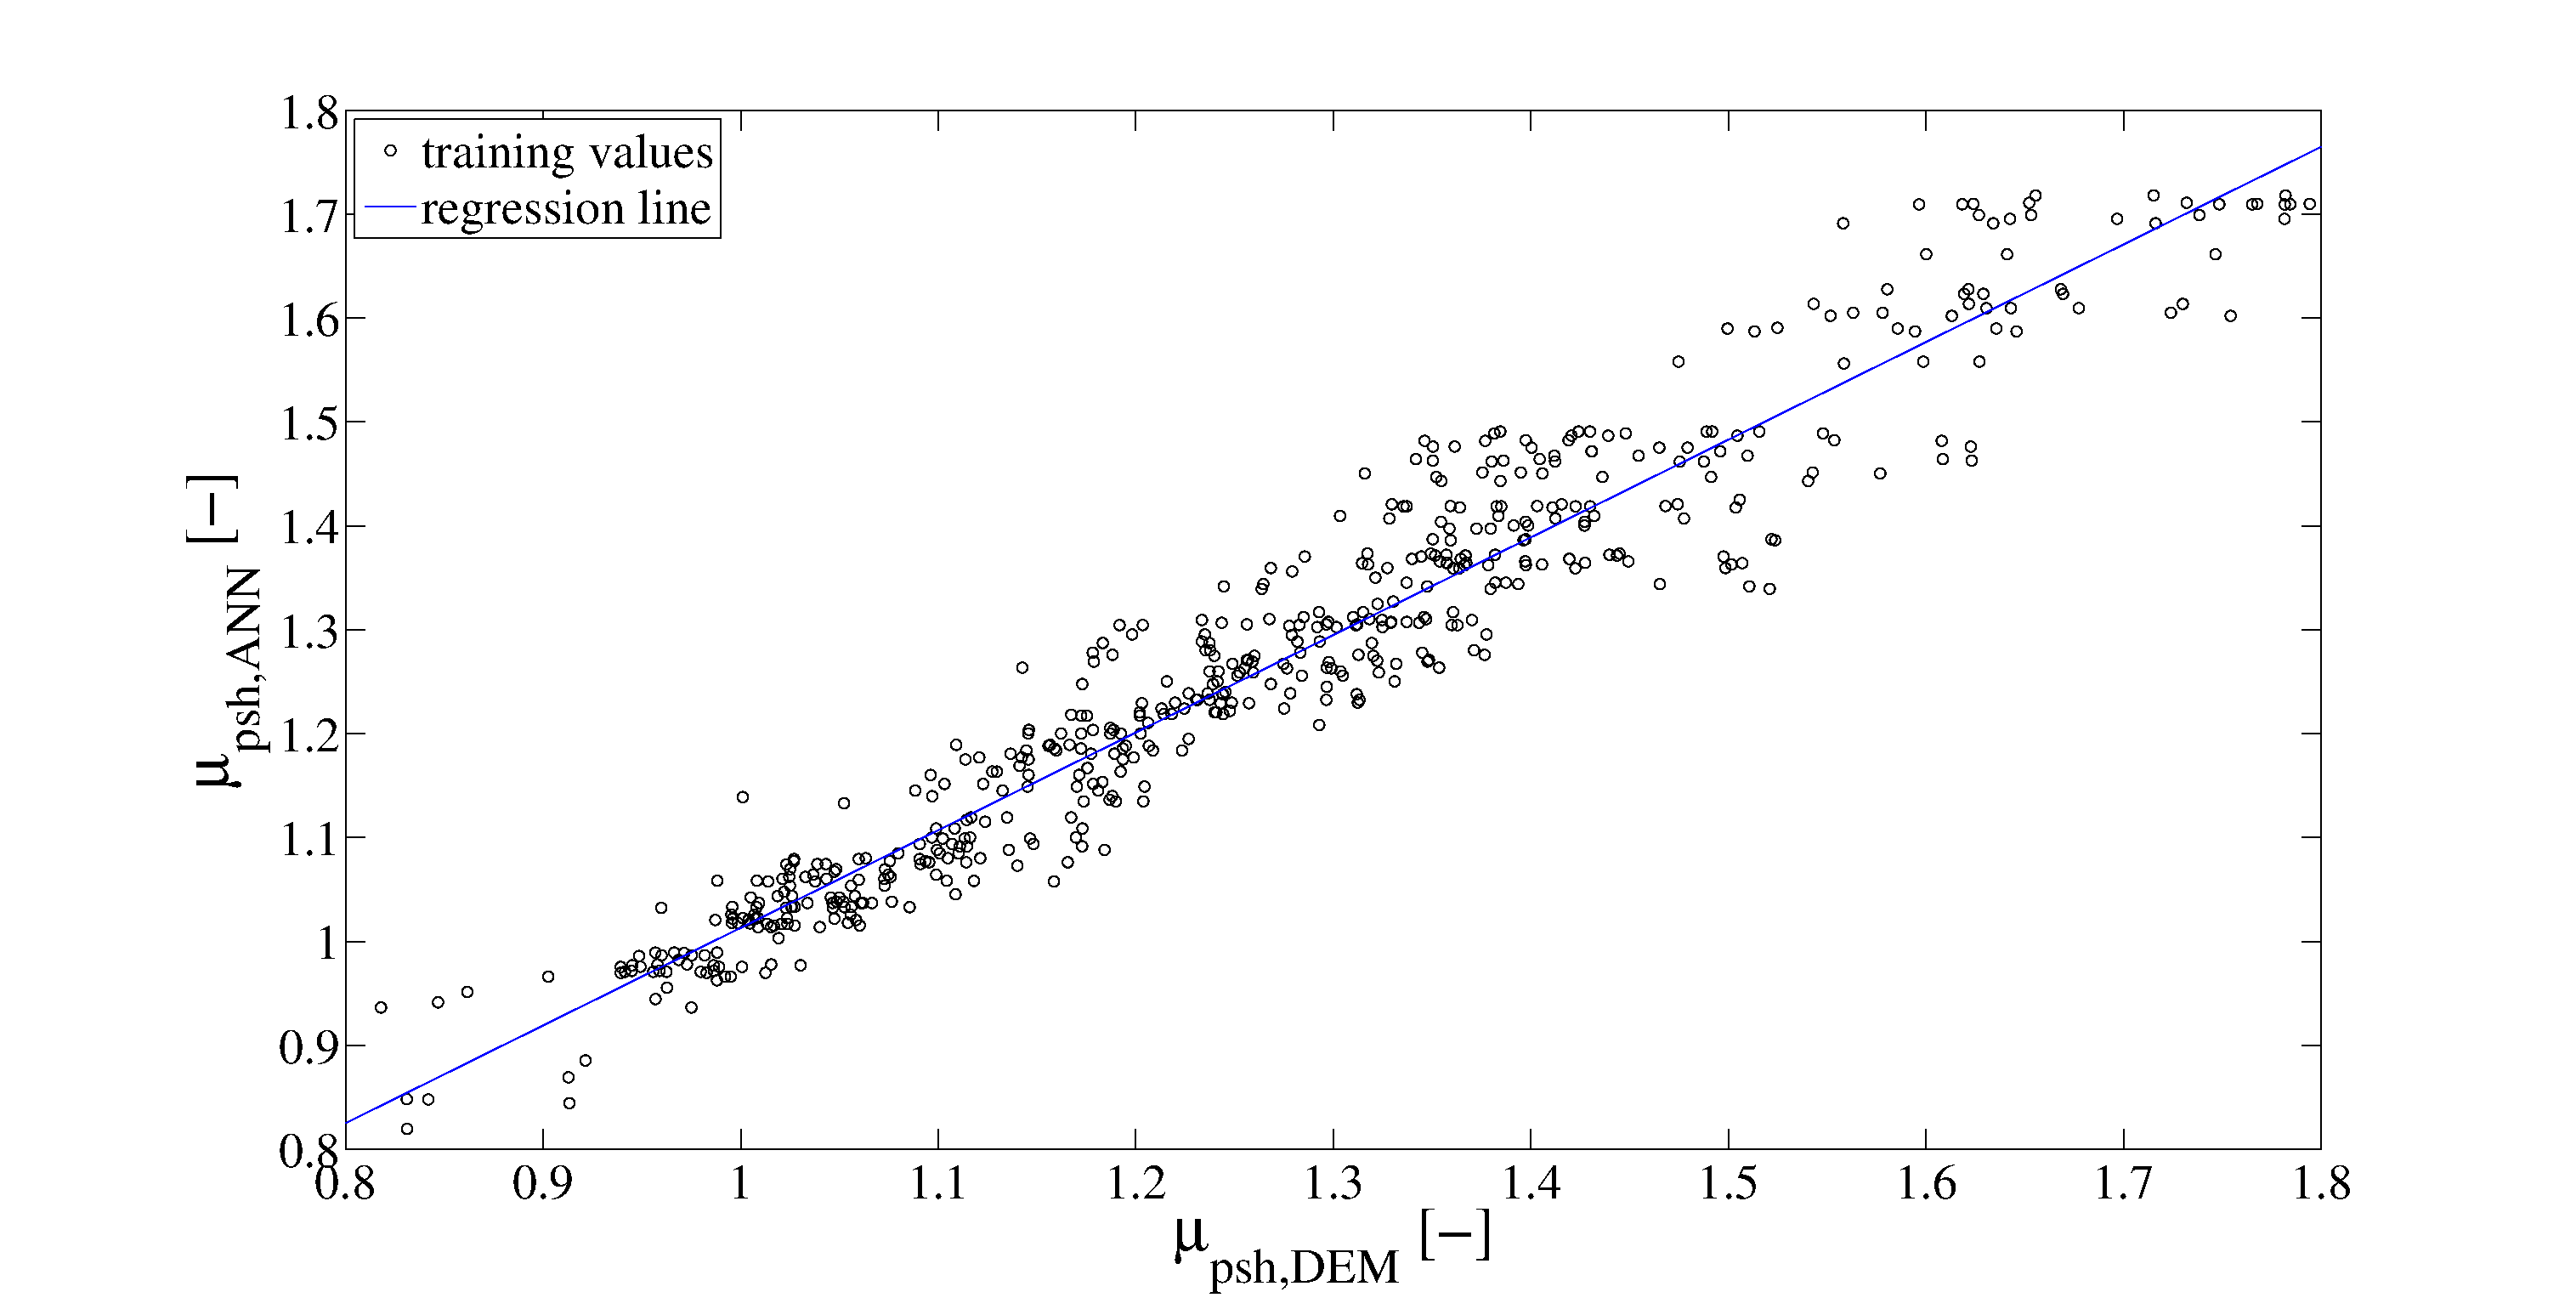
\includegraphics[width=.80\columnwidth]{images/022regression.eps}
%[width=.96\textwidth]
\caption[Comparison between prediction of the trained ANN and full DEM
simulation]{Comparison between prediction of the trained Artificial Neural
Network (\acs{ANN}) and 546 
\wrong{write down all the simulations performed at the end.}
full DEM simulations of the coefficient of pre-shear
(\acs{mupsh}).}
\label{fig:022regression} 
\end{figure}
\begin{table}[htbp] 
 \centering 
\begin{tabular}{l|cccccccccc} 
 \hline 
   &    \multicolumn{10}{l}{Weights of connection between input and hidden layer}  \\ 
 Neurons & 1 &  2 &  3 &  4 &  5 &  6 &  7 &  8 & 9 & 10 \\ 
 \hline 
  & 1.583 &  -0.543 &  -0.135 &  -0.462 &  1.370 &  1.048 &  1.025 &  -0.542 &  -0.162 &  -0.499 \\ 
  & -0.062 &  -0.576 &  -0.107 &  -1.246 &  -0.362 &  -0.239 &  1.078 &  1.156 &  0.161 &  0.919 \\ 
  & -0.057 &  0.265 &  0.552 &  -0.660 &  -0.006 &  1.021 &  0.139 &  -0.415 &  1.115 &  0.920 \\ 
  & 1.618 &  1.564 &  0.398 &  0.693 &  0.865 &  -0.047 &  0.535 &  -0.450 &  -0.558 &  -1.034 \\ 
  & 0.341 &  -0.028 &  -2.021 &  -1.331 &  0.899 &  -0.052 &  1.293 &  0.258 &  -1.550 &  0.786 \\ 
  & 0.309 &  0.682 &  0.277 &  -0.250 &  0.885 &  1.141 &  0.587 &  -0.825 &  -0.497 &  -0.054 \\ 
  & -0.186 &  0.950 &  -0.373 &  -0.218 &  0.355 &  -0.815 &  0.072 &  1.283 &  0.576 &  -0.740 \\ 
\hline 
   &    \multicolumn{10}{l}{Weights of connection between hidden and output layer}  \\ 
  & -0.200 &  -0.496 &  0.260 &  -0.210 &  0.061 &  0.023 &  0.202 &  0.033 &  0.079 &  0.167 \\ 
\hline 
   &    \multicolumn{10}{l}{Biases of hidden layer}  \\ 
  & -1.906 &  2.073 &  1.657 &  1.479 &  -1.280 &  -1.119 &  -0.770 &  0.569 &  0.345 &  -0.075 \\ 
\hline
\hline  
   &    \multicolumn{10}{l}{Weights of connection between input and hidden layer}  \\ 
 Neurons & 11 &  12 &  13 &  14 &  15 &  16 &  17 &  18 & 19 & 20 \\ 
 \hline 
  & -0.154 &  -0.126 &  -0.303 &  0.798 &  -1.191 &  -0.704 &  -0.254 &  -0.988 &  0.788 &  -0.612 \\ 
  & -0.292 &  0.715 &  1.266 &  -0.506 &  0.074 &  -1.095 &  -1.565 &  -1.085 &  -0.968 &  -0.073 \\ 
  & -0.443 &  1.142 &  0.342 &  -0.198 &  0.545 &  -0.202 &  0.722 &  -0.577 &  -1.573 &  -0.440 \\ 
  & 0.918 &  0.458 &  -1.031 &  -0.916 &  -0.092 &  0.312 &  0.935 &  -0.390 &  -0.489 &  -1.510 \\ 
  & -0.612 &  0.922 &  1.412 &  -0.305 &  -0.120 &  -0.696 &  -0.396 &  0.834 &  0.908 &  -0.022 \\ 
  & -1.047 &  -1.113 &  0.228 &  1.605 &  -0.899 &  -1.168 &  -0.017 &  -0.081 &  0.341 &  0.876 \\ 
  & -1.320 &  0.114 &  -0.233 &  -0.013 &  1.191 &  0.087 &  -0.527 &  1.106 &  0.266 &  0.877 \\ 
\hline 
   &    \multicolumn{10}{l}{Weights of connection between hidden and output layer}  \\ 
  & -0.082 &  0.173 &  -0.419 &  0.054 &  0.023 &  -0.056 &  -0.181 &  -0.150 &  0.167 &  -0.580 \\ 
\hline 
   &    \multicolumn{10}{l}{Biases of hidden layer}  \\ 
  & -0.231 &  -0.508 &  0.435 &  0.813 &  -1.221 &  -1.386 &  -1.356 &  -1.671 &  1.700 &  -2.221 \\ 
\hline 
\hline 
   &    \multicolumn{10}{l}{Biases of output layer}  \\ 
 &    \multicolumn{10}{c}{-0.543}  \\ 
\hline 
 \end{tabular} 
\caption[Weights and biases table for the coefficient of internal friction
for sinter fine]{Weights and biases table for the coefficient of internal
friction for sinter fine.}
\label{tab:originalsinterfinesct} 
\end{table}
\begin{table}[htbp] 
 \centering 
\begin{tabular}{l|ccccccccc} 
 \hline 
   &    \multicolumn{9}{l}{Weights of connection between input and hidden layer}  \\ 
 Neurons & 1 &  2 &  3 &  4 &  5 &  6 &  7 &  8 & 9 \\ 
 \hline 
  & 0.148 &  -0.064 &  -0.585 &  -1.247 &  1.264 &  0.108 &  -0.335 &  -0.950 &  0.722 \\ 
  & 1.889 &  1.334 &  -0.105 &  1.016 &  1.781 &  -0.652 &  -1.664 &  1.497 &  -0.578 \\ 
  & -0.271 &  1.221 &  1.086 &  0.777 &  0.298 &  0.984 &  0.101 &  -1.466 &  -0.230 \\ 
  & -1.316 &  0.385 &  -1.997 &  -1.531 &  -1.159 &  1.877 &  1.227 &  0.948 &  1.643 \\ 
\hline 
   &    \multicolumn{9}{l}{Weights of connection between hidden and output layer}  \\ 
  & 0.137 &  0.437 &  -0.575 &  -0.025 &  0.109 &  -0.667 &  -0.184 &  0.119 &  0.806 \\ 
\hline 
   &    \multicolumn{9}{l}{Biases of hidden layer}  \\ 
  & -2.453 &  2.311 &  1.399 &  0.679 &  0.108 &  0.844 &  -1.614 &  -1.674 &  2.654 \\ 
\hline 
   &    \multicolumn{9}{l}{Biases of output layer}  \\ 
 &    \multicolumn{9}{c}{-0.494}  \\ 
\hline 
 \end{tabular} 
\caption[Weights and biases table for sinter fine AoR]{Weights and biases table
for sinter fine \acs{AoR}.}
\label{tab:35weightssinterfineaor} 
\end{table}

\section{Statistical tools comparison}
\label{sec:statisticaltoolscomparison}

%\begin{figure}[htbp]
  %\null\hfill
  \subfloat[SCT Bayesian linear regressor.]{
	  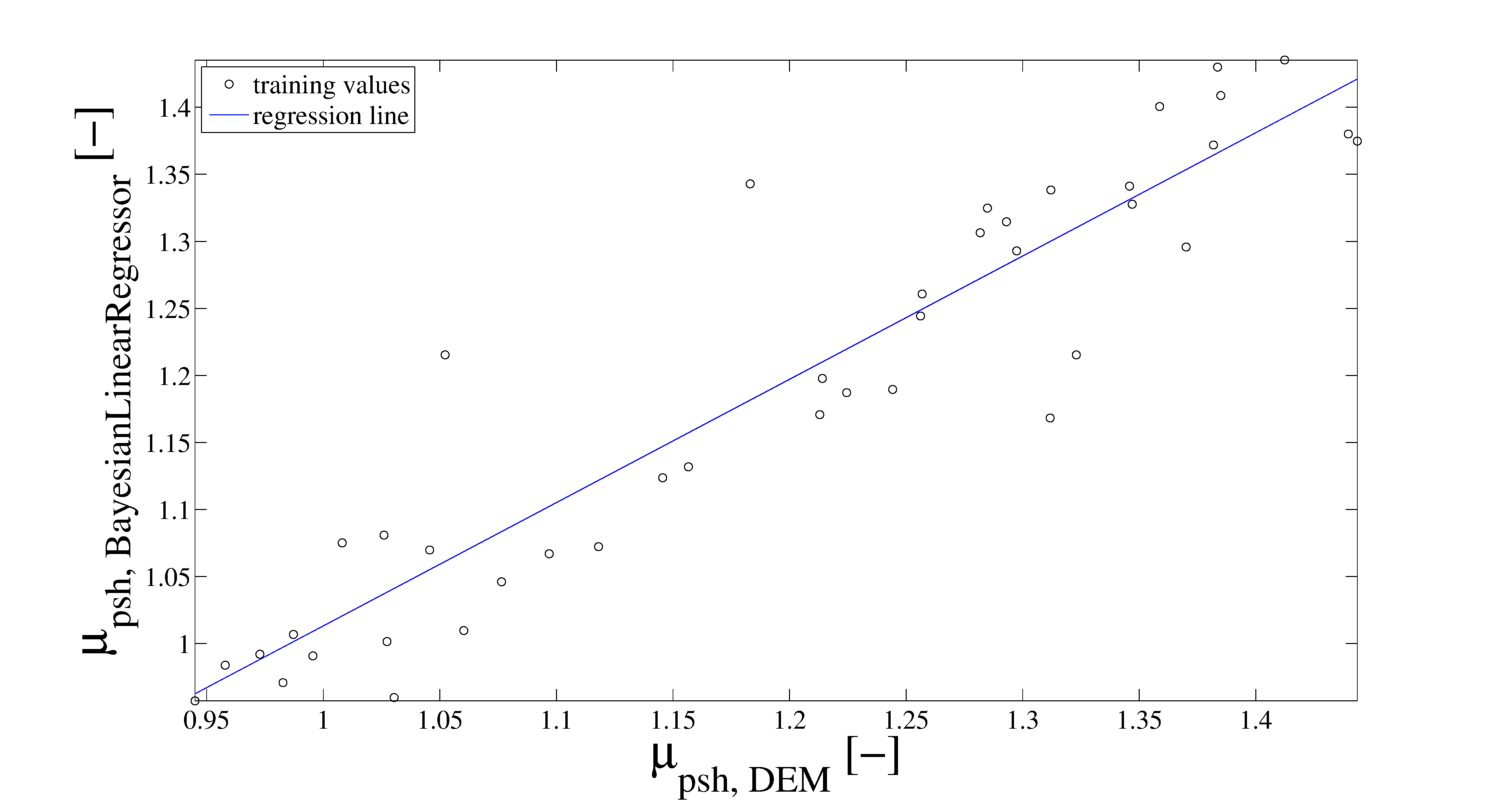
\includegraphics[width=.48\columnwidth]{images/069sctbayesianlinearregressor}
	  \label{fig:069sctbayesianlinearregressor}
  }
  \quad
    \subfloat[SCT Gaussian non linear regressor.]{
	  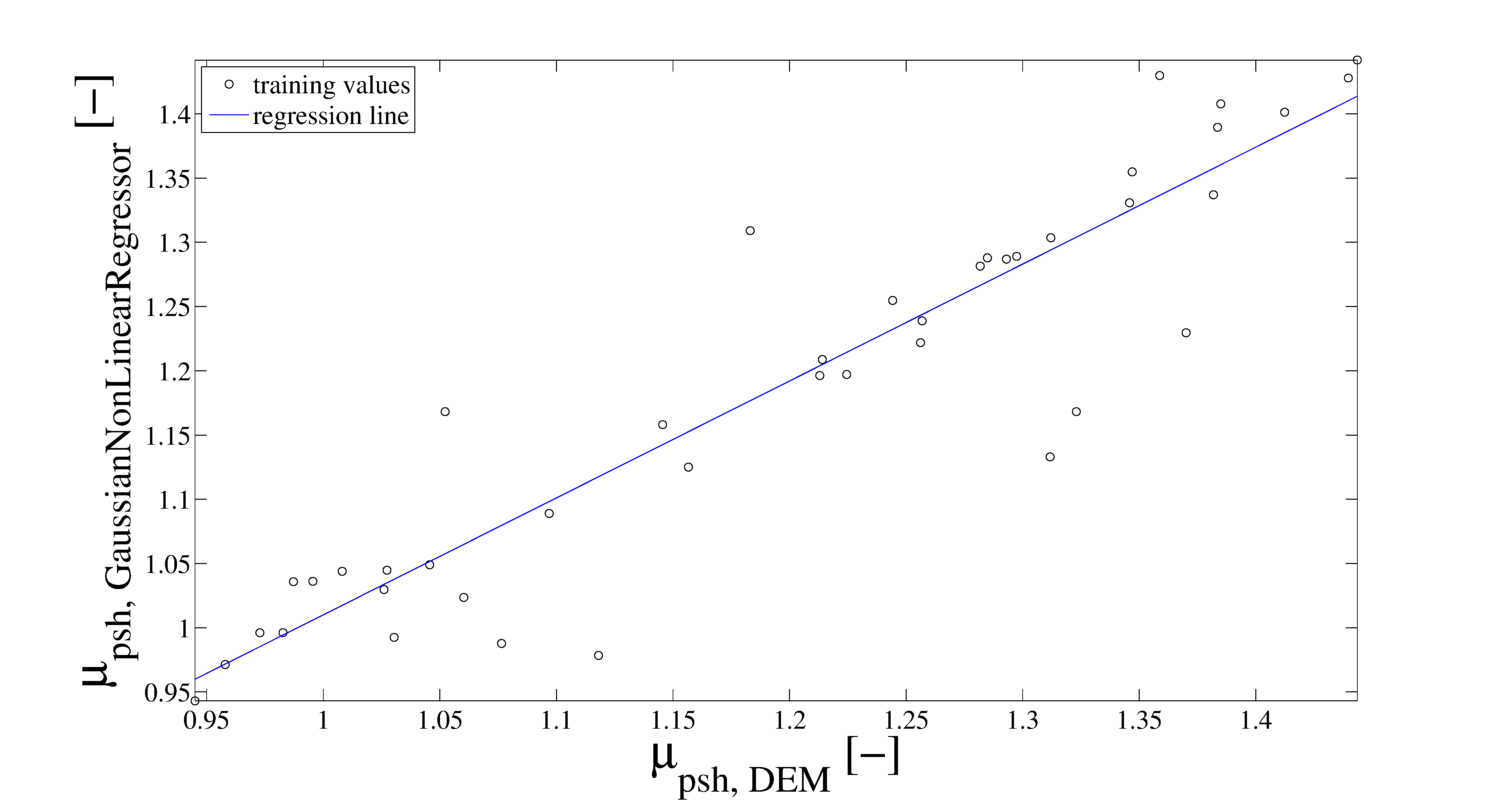
\includegraphics[width=.48\columnwidth]{images/070sctgaussiannonlinearregressor}
	  \label{fig:070sctgaussiannonlinearregressor}
  }
  \\
 % \hfill
  \subfloat[SCT ANN non linear regression.]{
	  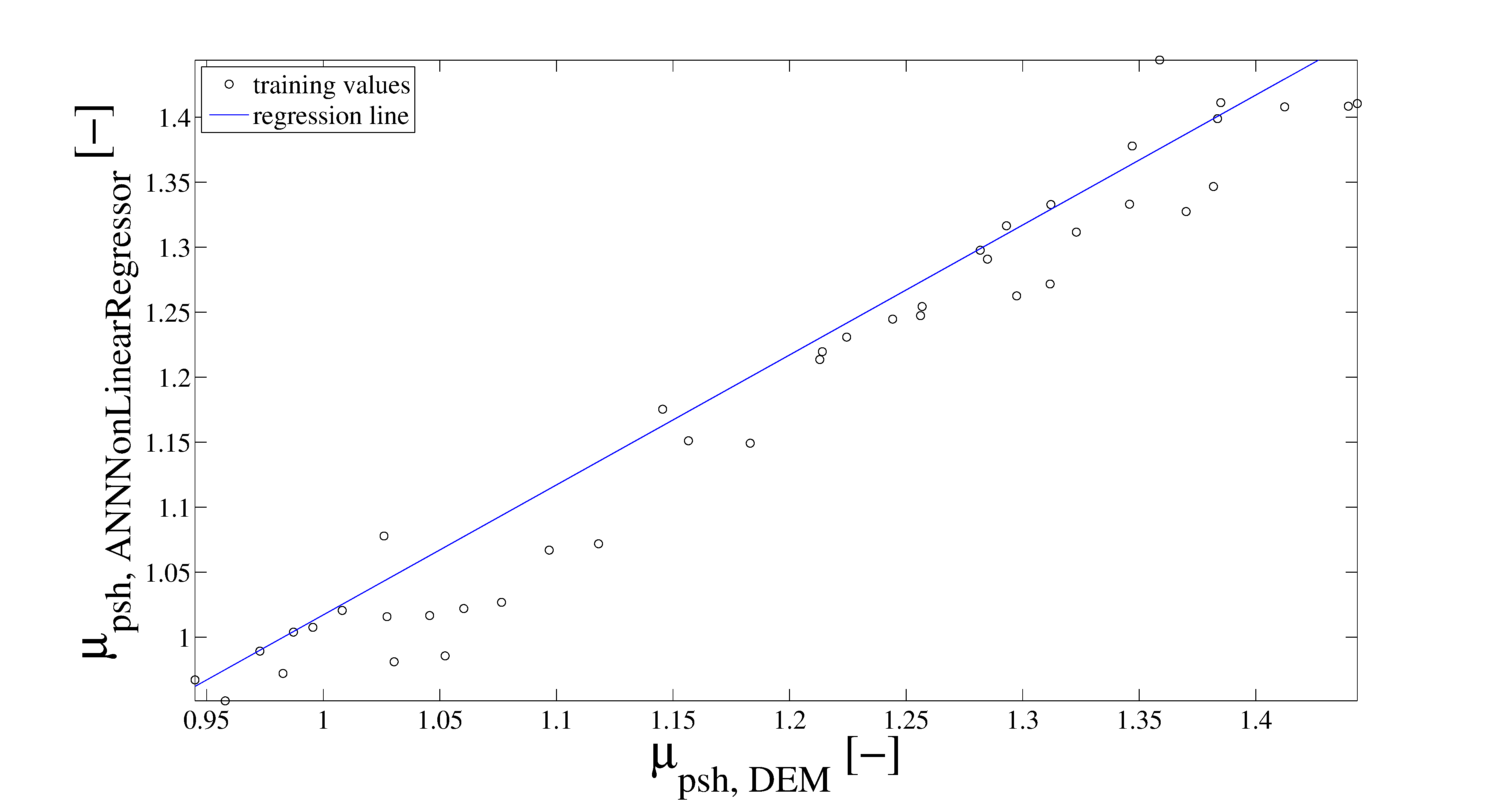
\includegraphics[width=.48\columnwidth]{images/071annnonlinearregressor}
	  \label{fig:071annnonlinearregressor}
  }
  \quad
    \subfloat[AoR Bayesian linear regressor.]{
	  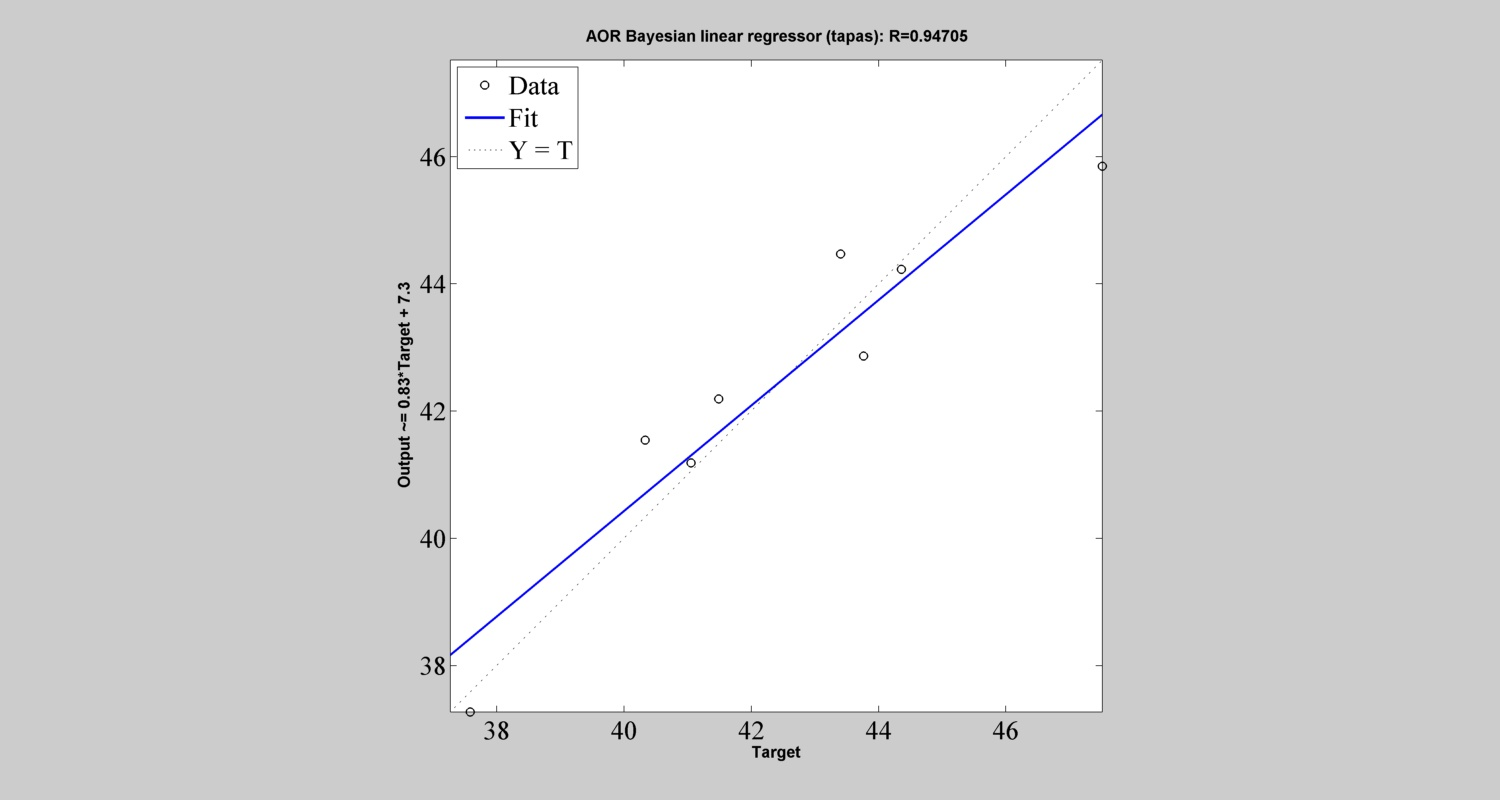
\includegraphics[width=.48\columnwidth]{images/072aorbayesianlinearregression}
	  \label{fig:072aorbayesianlinearregression}  }
  \\
    \subfloat[AoR Gaussian non linear regressor.]{
	  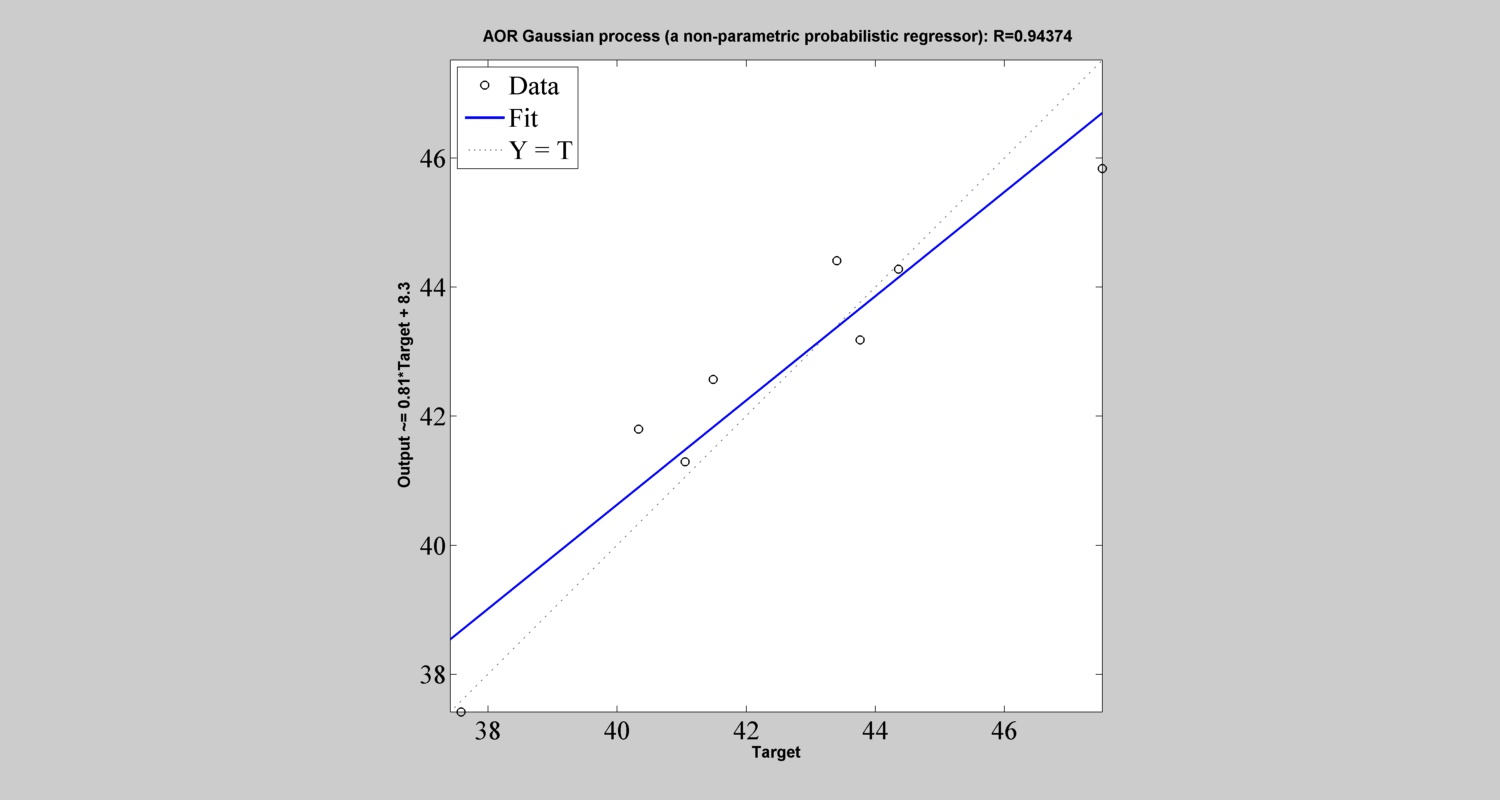
\includegraphics[width=.48\columnwidth]{images/073aorgaussiannonlinearregression}
	  \label{fig:073aorgaussiannonlinearregression}
  }
  \quad
 % \hfill
  \subfloat[AoR ANN non linear regression.]{
	  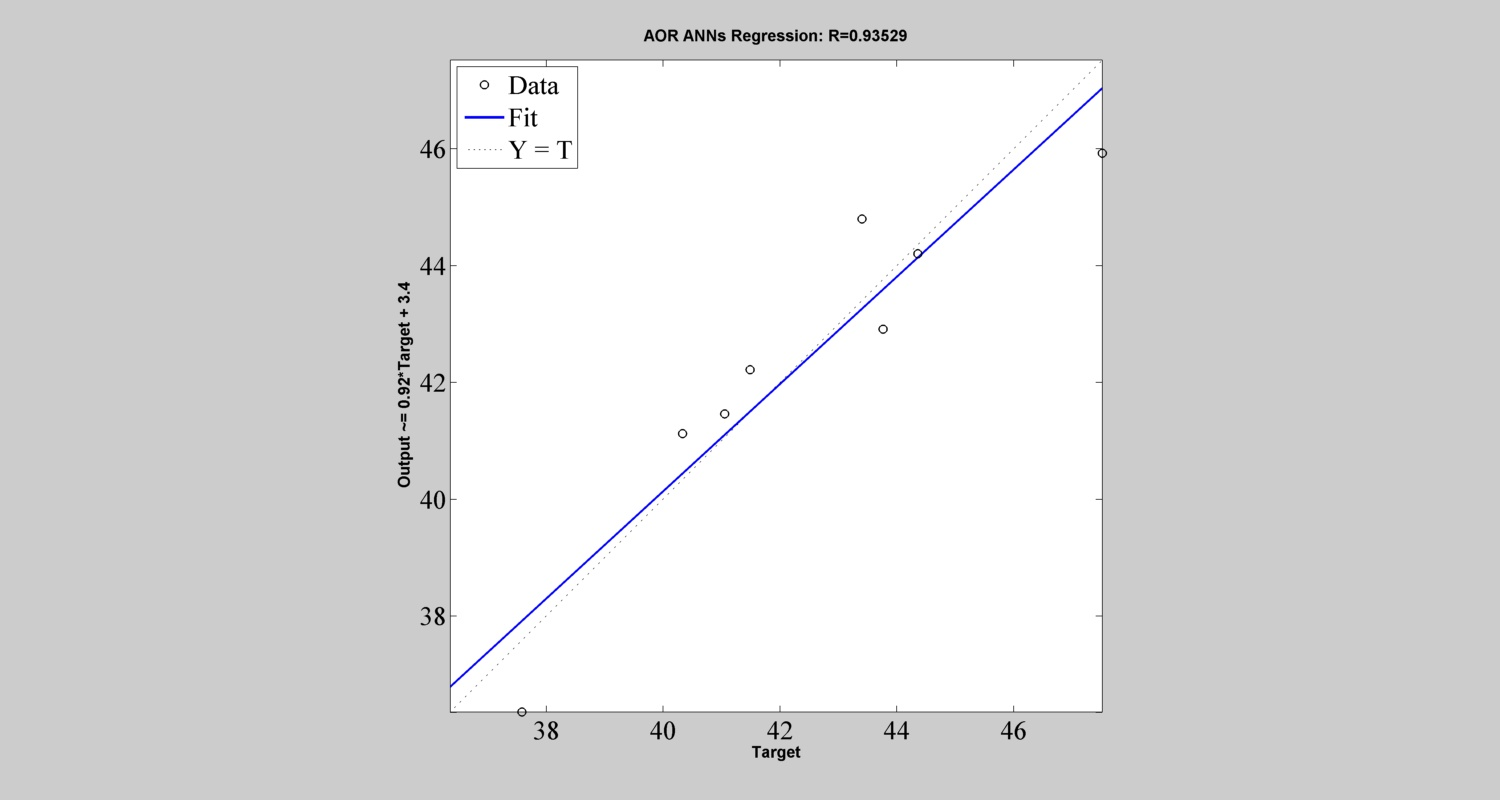
\includegraphics[width=.48\columnwidth]{images/074aorannnonlinearegression}
	  \label{fig:074aorannnonlinearegression}
  }
 % \hfill\null
  \caption{Regressions.}
  \label{fig:077regressions}
\end{figure}

% \begin{figure}%[!h] 
% \centering 
% 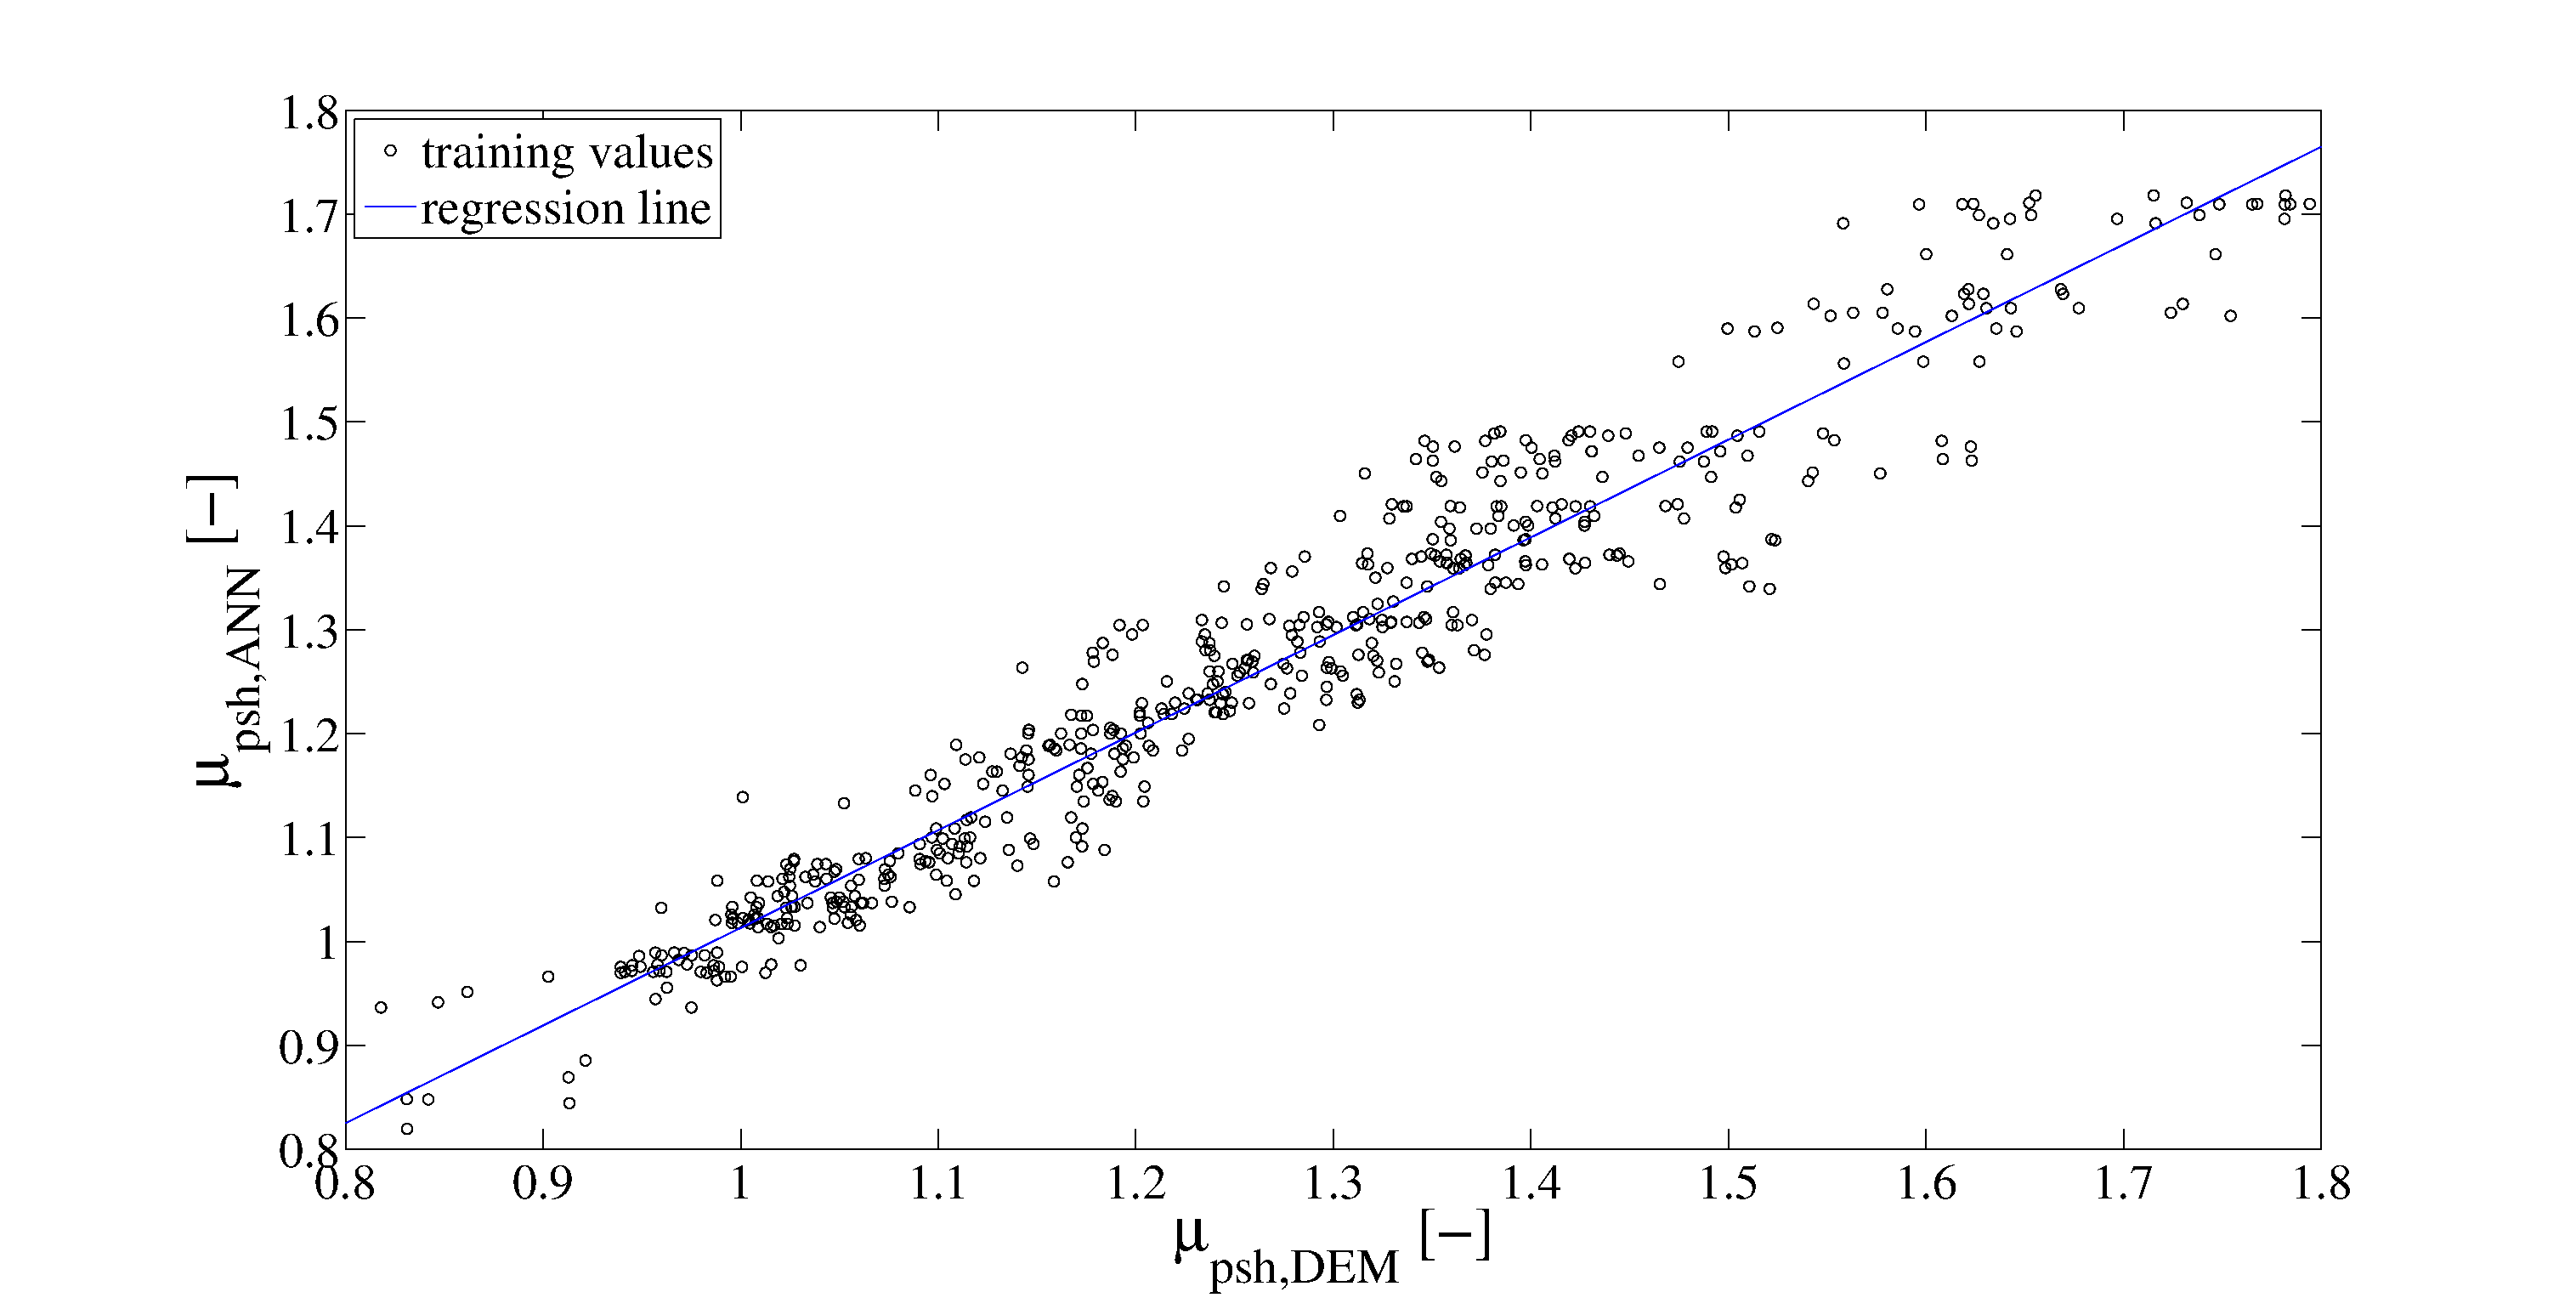
\includegraphics[width=.80\columnwidth]{images/022regression.eps}
% %[width=.48\textwidth]
% \caption[Comparison between prediction of the trained ANN and full DEM
% simulation]{Comparison between prediction of the trained Artificial Neural
% Network ($ANN$) and 546 
% \wrong{write down all the simulations performed at the end.}
% full DEM simulations of the coefficient of pre-shear
% (\ac{mupsh}).}
% \label{fig:022regression} 
% \end{figure}
\begin{figure}[htbp]
	\centering
  %\null\hfill
  \subfloat[SCT Bayesian linear regressor.]{
	  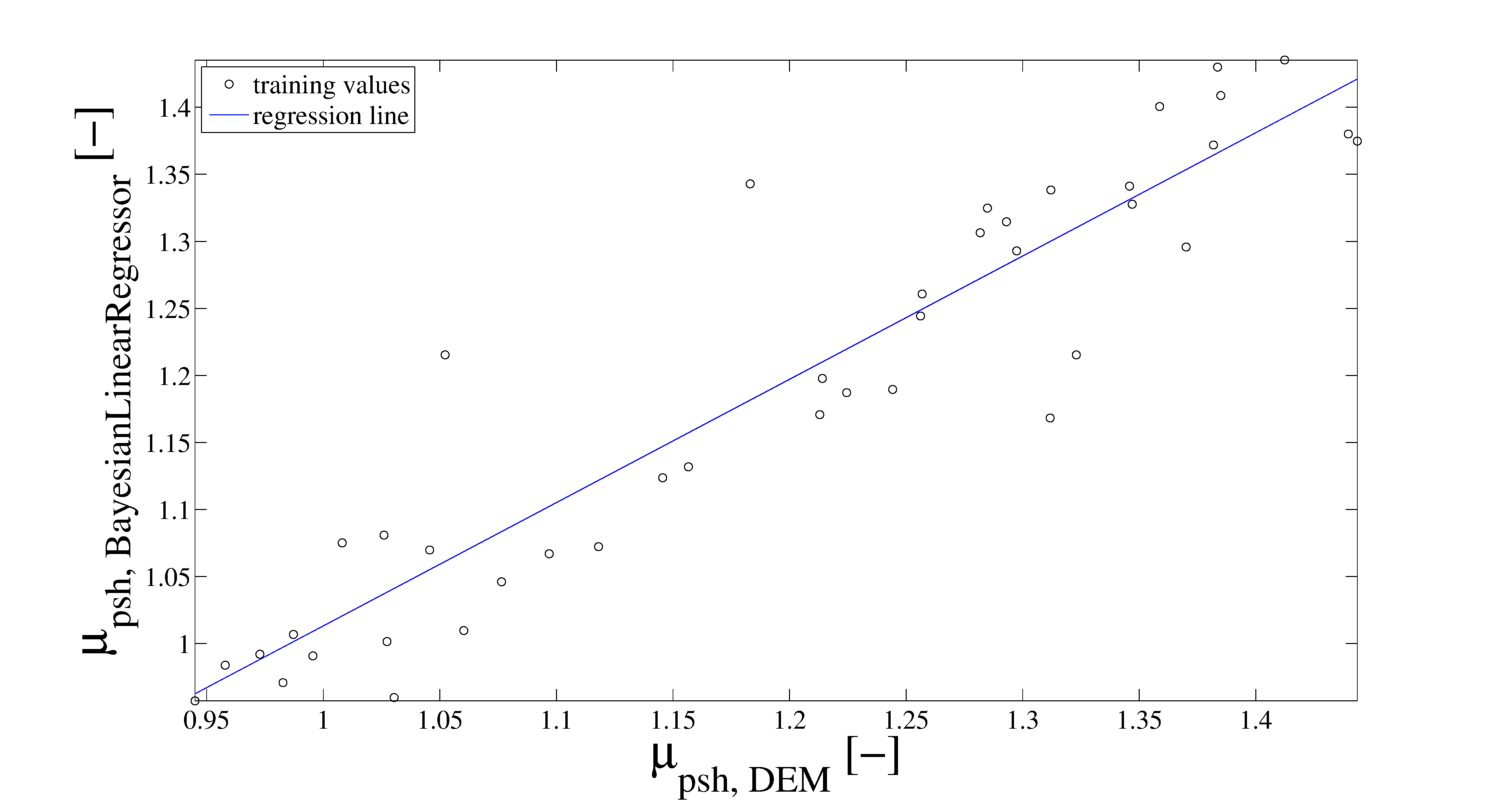
\includegraphics[width=.75\columnwidth]{images/137SCTBayesianLinearRegressor}
	  \label{fig:137SCTBayesianLinearRegressor}
  }
  \\
    \subfloat[SCT Gaussian non linear regressor.]{
	  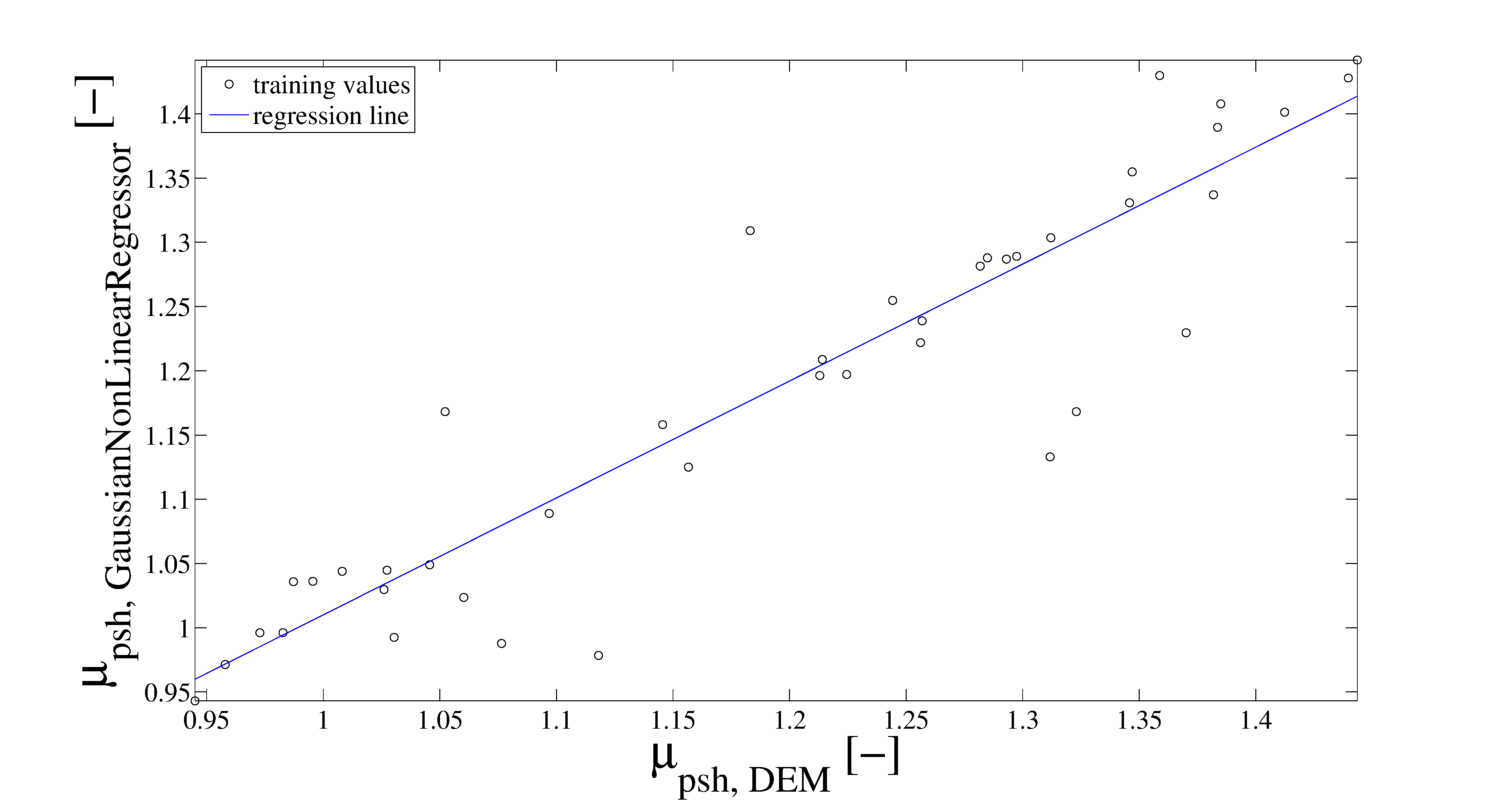
\includegraphics[width=.75\columnwidth]{images/138SCTGaussianNonLinearRegressor}
	  \label{fig:138SCTGaussianNonLinearRegressor}
  }
  \\
 % \hfill
  \subfloat[SCT ANN non linear regression.]{
	  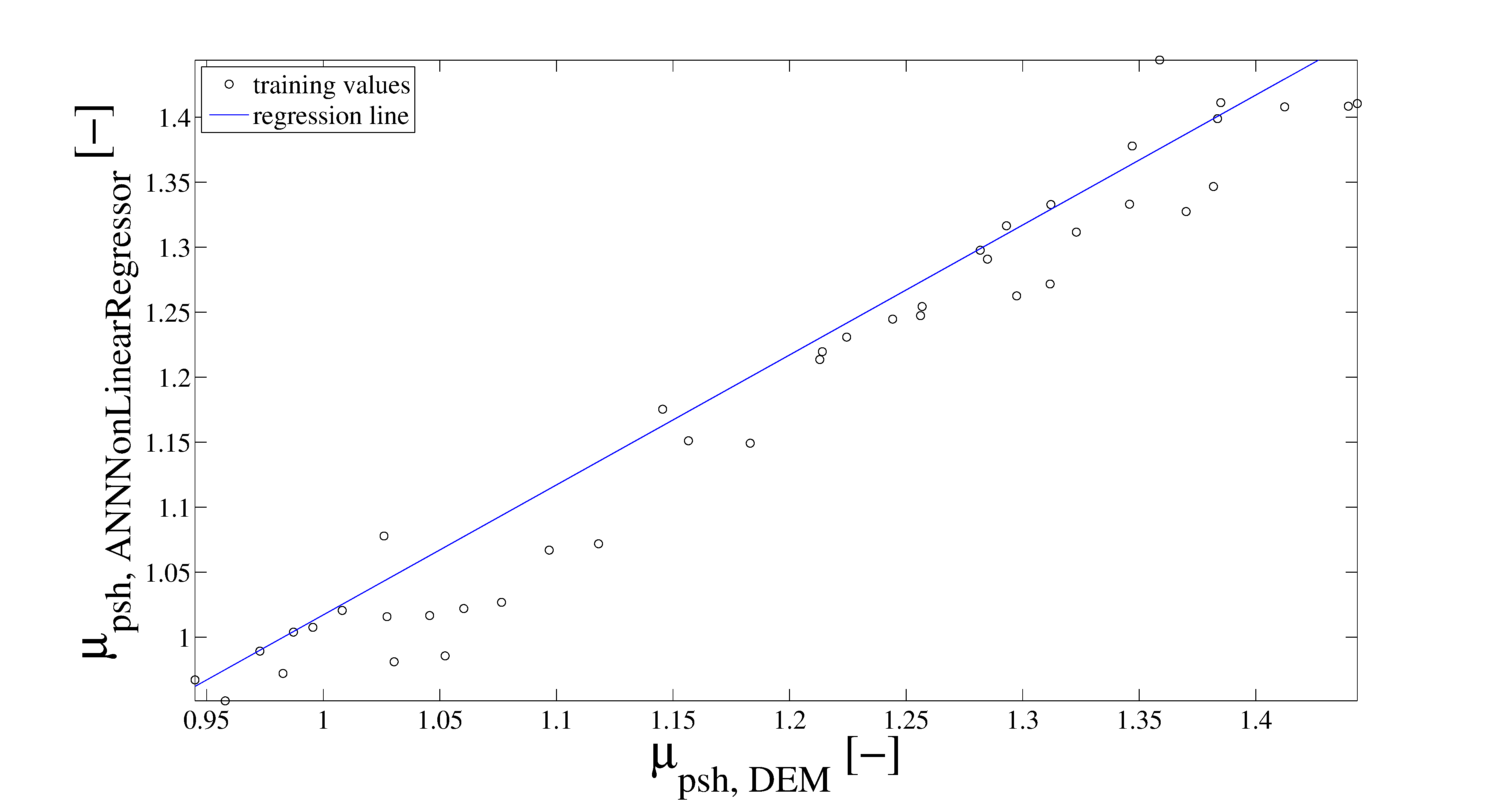
\includegraphics[width=.75\columnwidth]{images/139SCTANNNonLinearRegressor}
	  \label{fig:139SCTANNNonLinearRegressor}
  }
  \caption{Regressions comparison for the \acs{mupsh}.}
  \label{fig:143sctregressions}
\end{figure}

% \begin{figure}%[!h] 
% \centering 
% 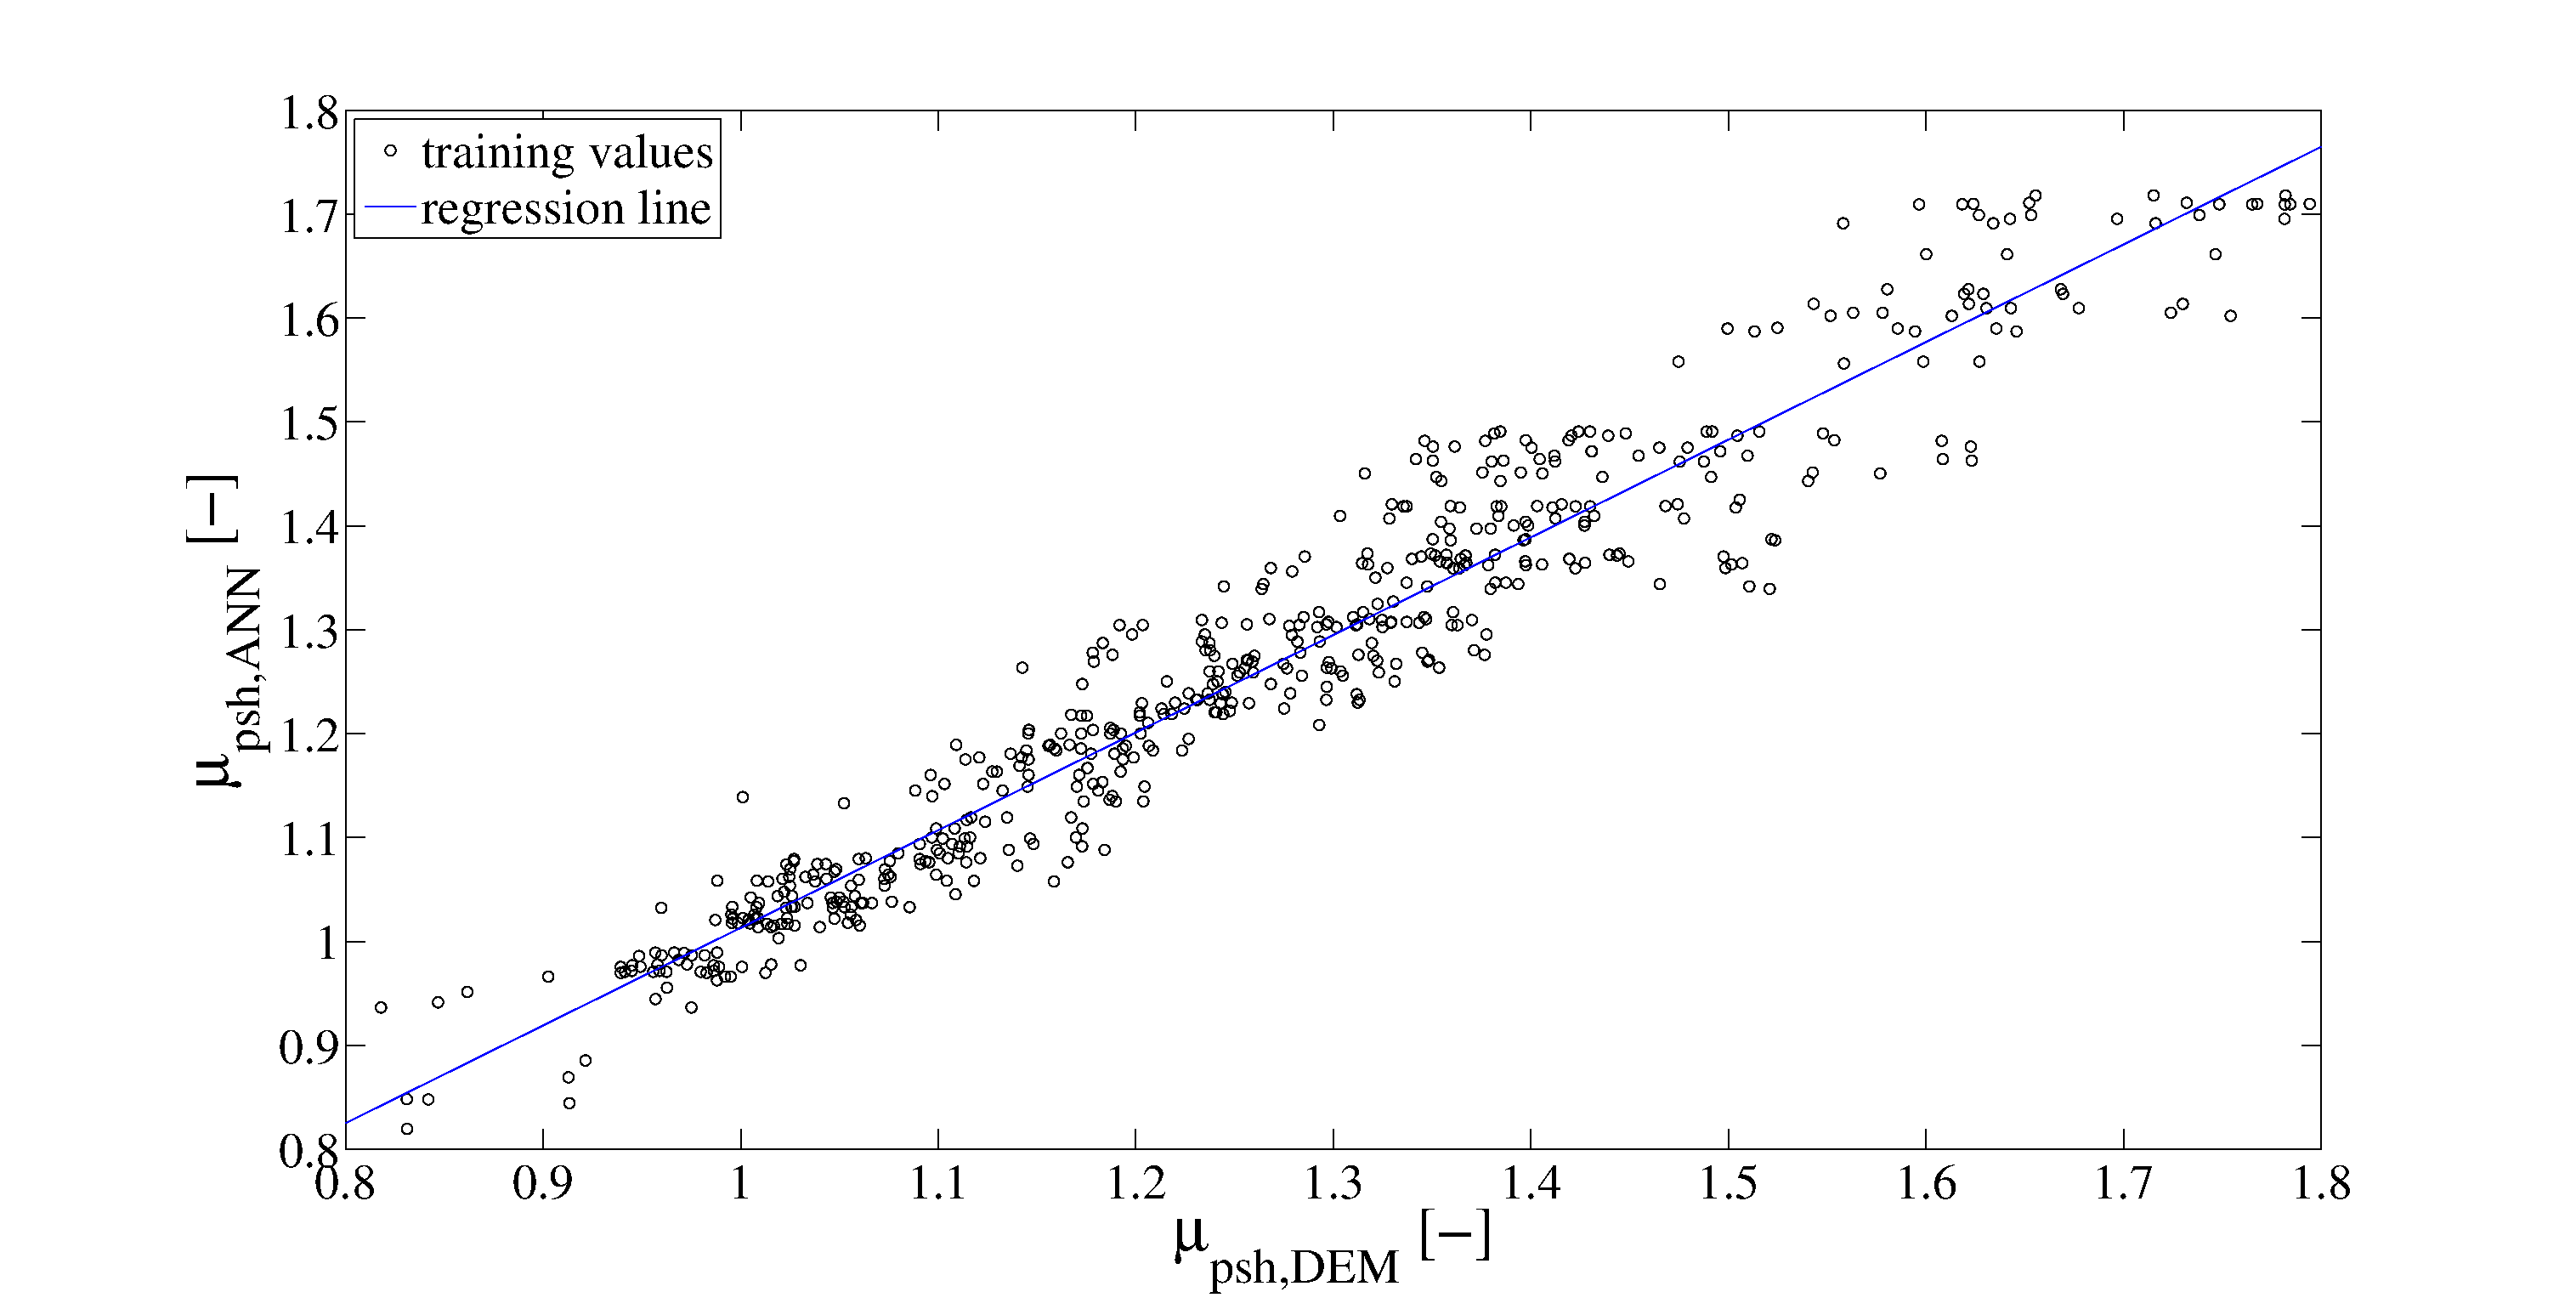
\includegraphics[width=.80\columnwidth]{images/022regression.eps}
% %[width=.48\textwidth]
% \caption[Comparison between prediction of the trained ANN and full DEM
% simulation]{Comparison between prediction of the trained Artificial Neural
% Network (\acs{ANN}) and 546 
% \wrong{write down all the simulations performed at the end.}
% full DEM simulations of the coefficient of pre-shear
% (\acs{mupsh}).}
% \label{fig:022regression} 
% \end{figure}
\begin{figure}[htbp]
	\centering

	 % \resizebox{12cm}{!}{\input{images/137SCTBayesianLinearRegressor.tikz}}


    \subfloat[AoR Bayesian linear regressor.]{
	  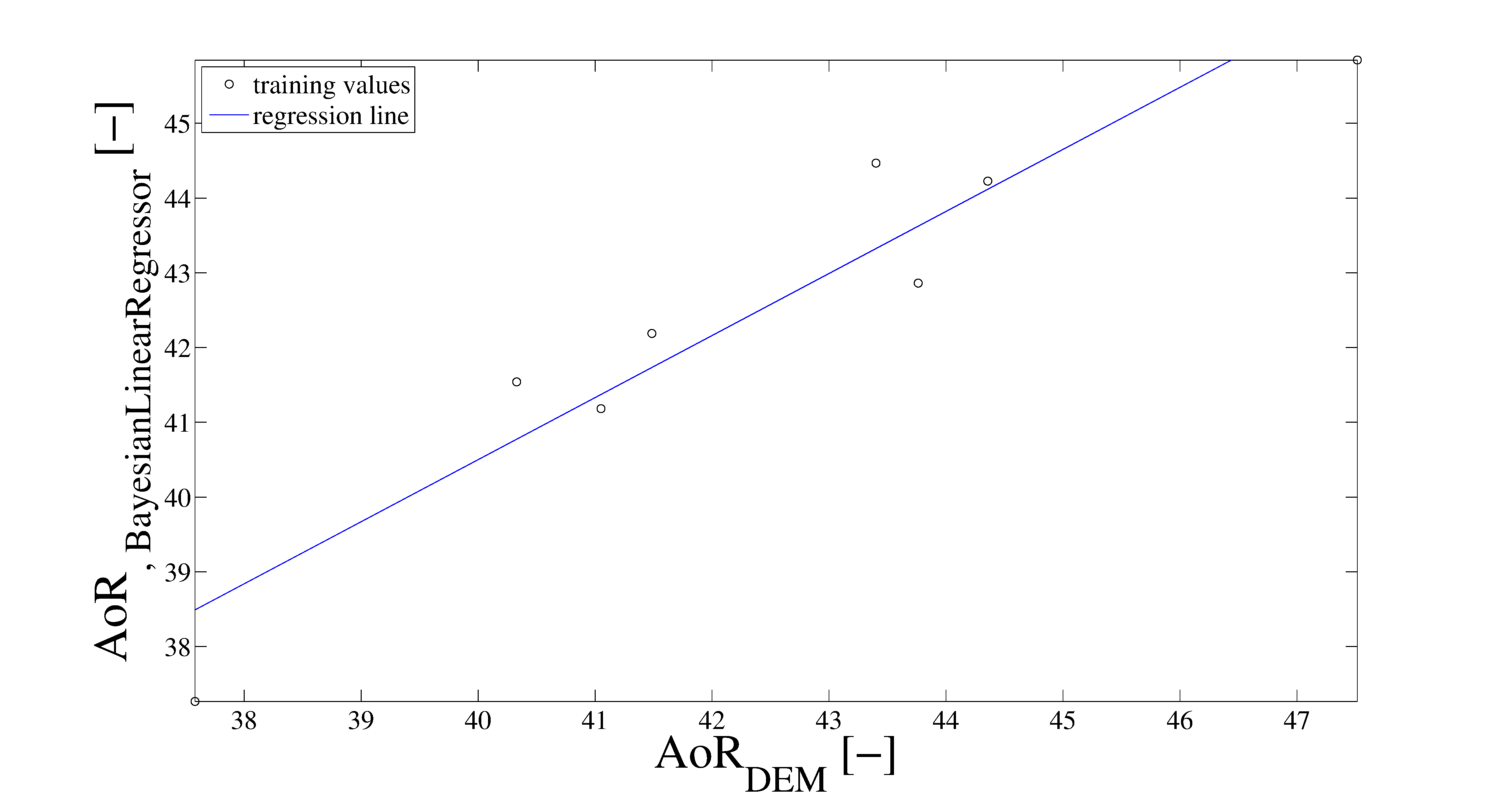
\includegraphics[width=.75\columnwidth]{images/140AoRBayesianLinearRegressor}
	  \label{fig:140AoRBayesianLinearRegressor}  }
  \\
    \subfloat[AoR Gaussian non linear regressor.]{
	  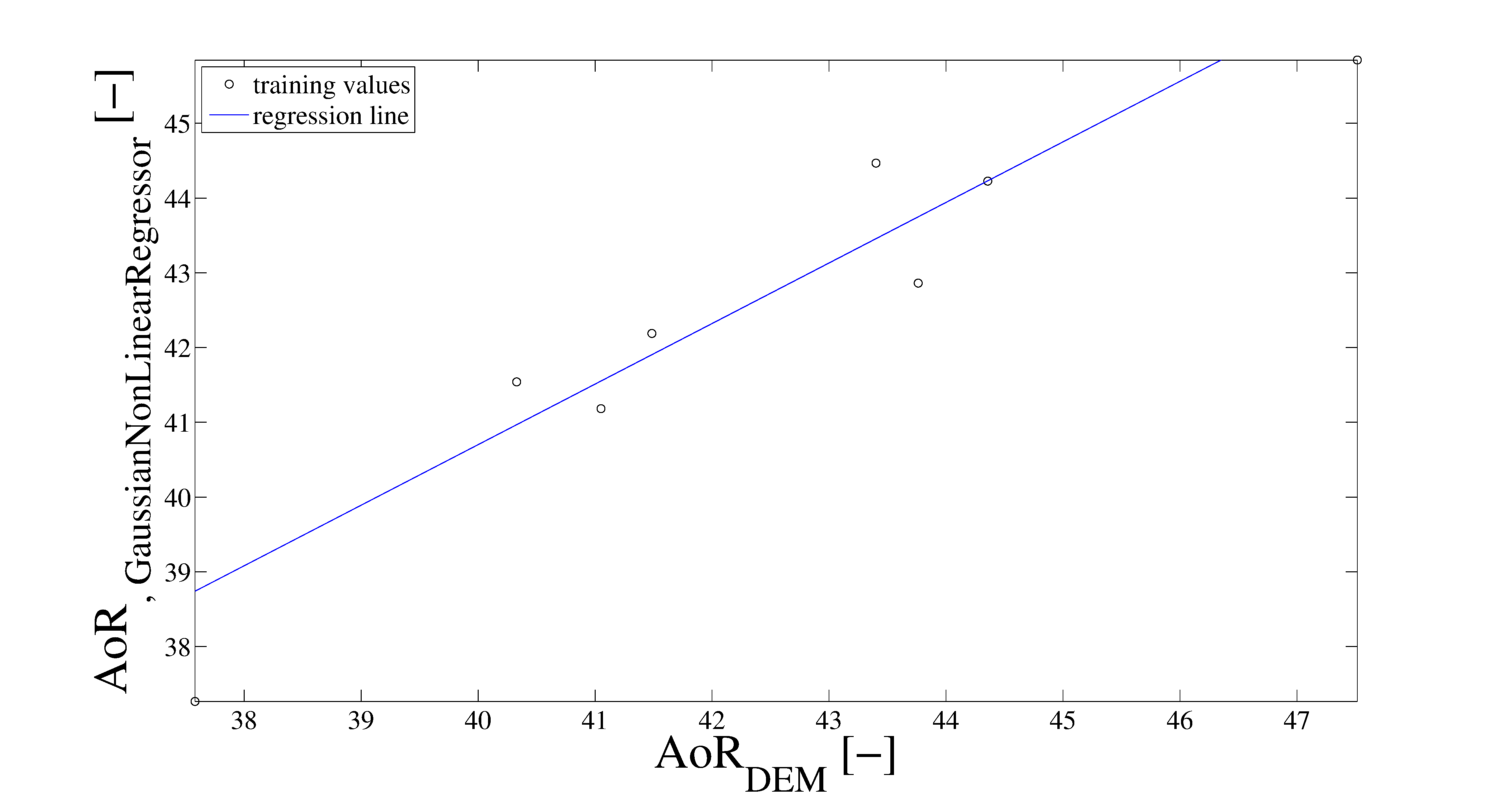
\includegraphics[width=.75\columnwidth]{images/141AoRGaussianNonLinearRegressor}
	  \label{fig:141AoRGaussianNonLinearRegressor}
  }
  \\
 % \hfill
  \subfloat[AoR ANN non linear regression.]{
	  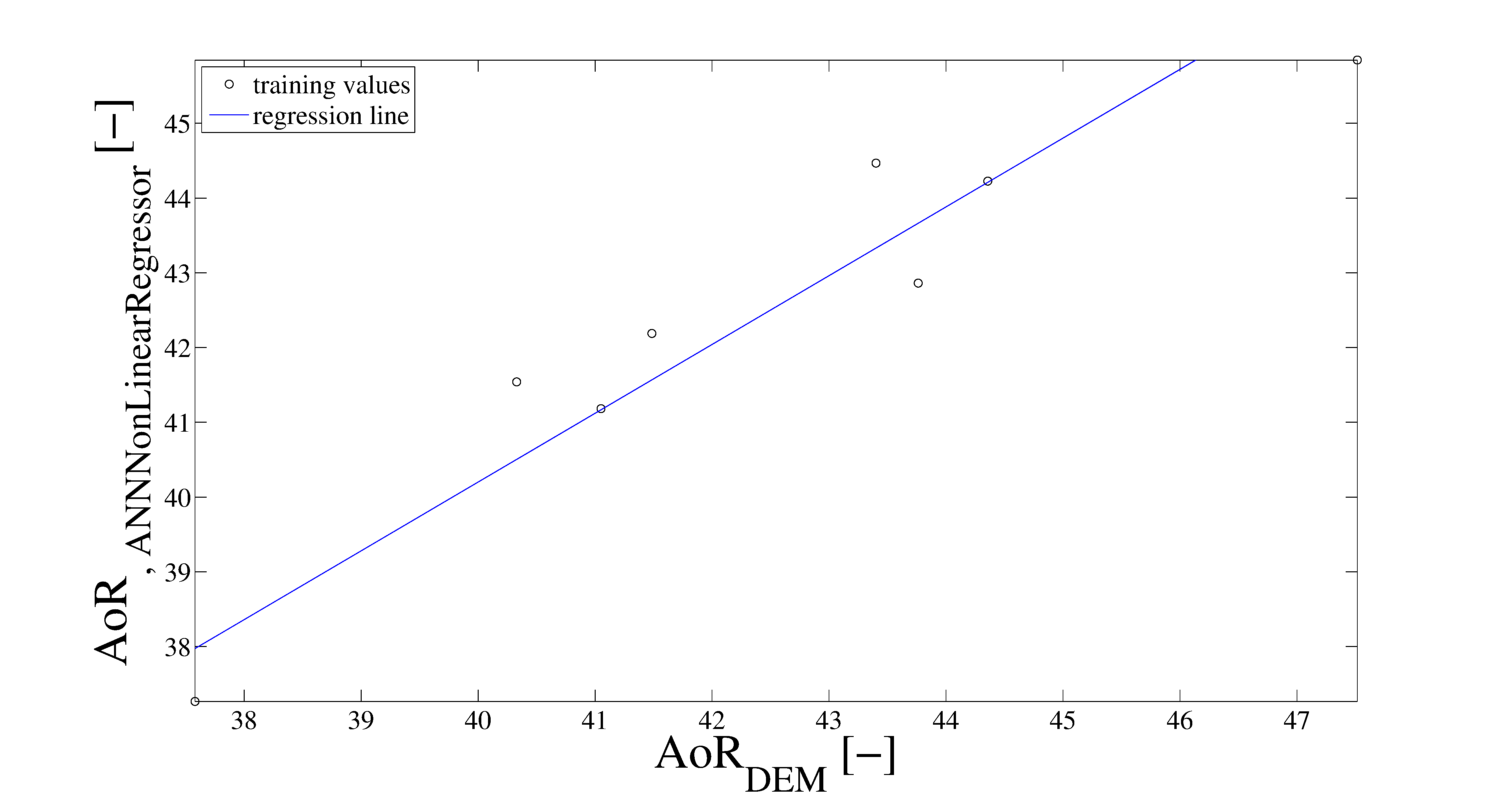
\includegraphics[width=.75\columnwidth]{images/142AoRANNNonLinearRegressor}
	  \label{fig:142AoRANNNonLinearRegressor}
  }
 % \hfill\null
  \caption{Regressions comparison for the \acs{AoR}.}
  \label{fig:144aorregressions}
\end{figure}

% \begin{figure}%[!h] 
% \centering 
% 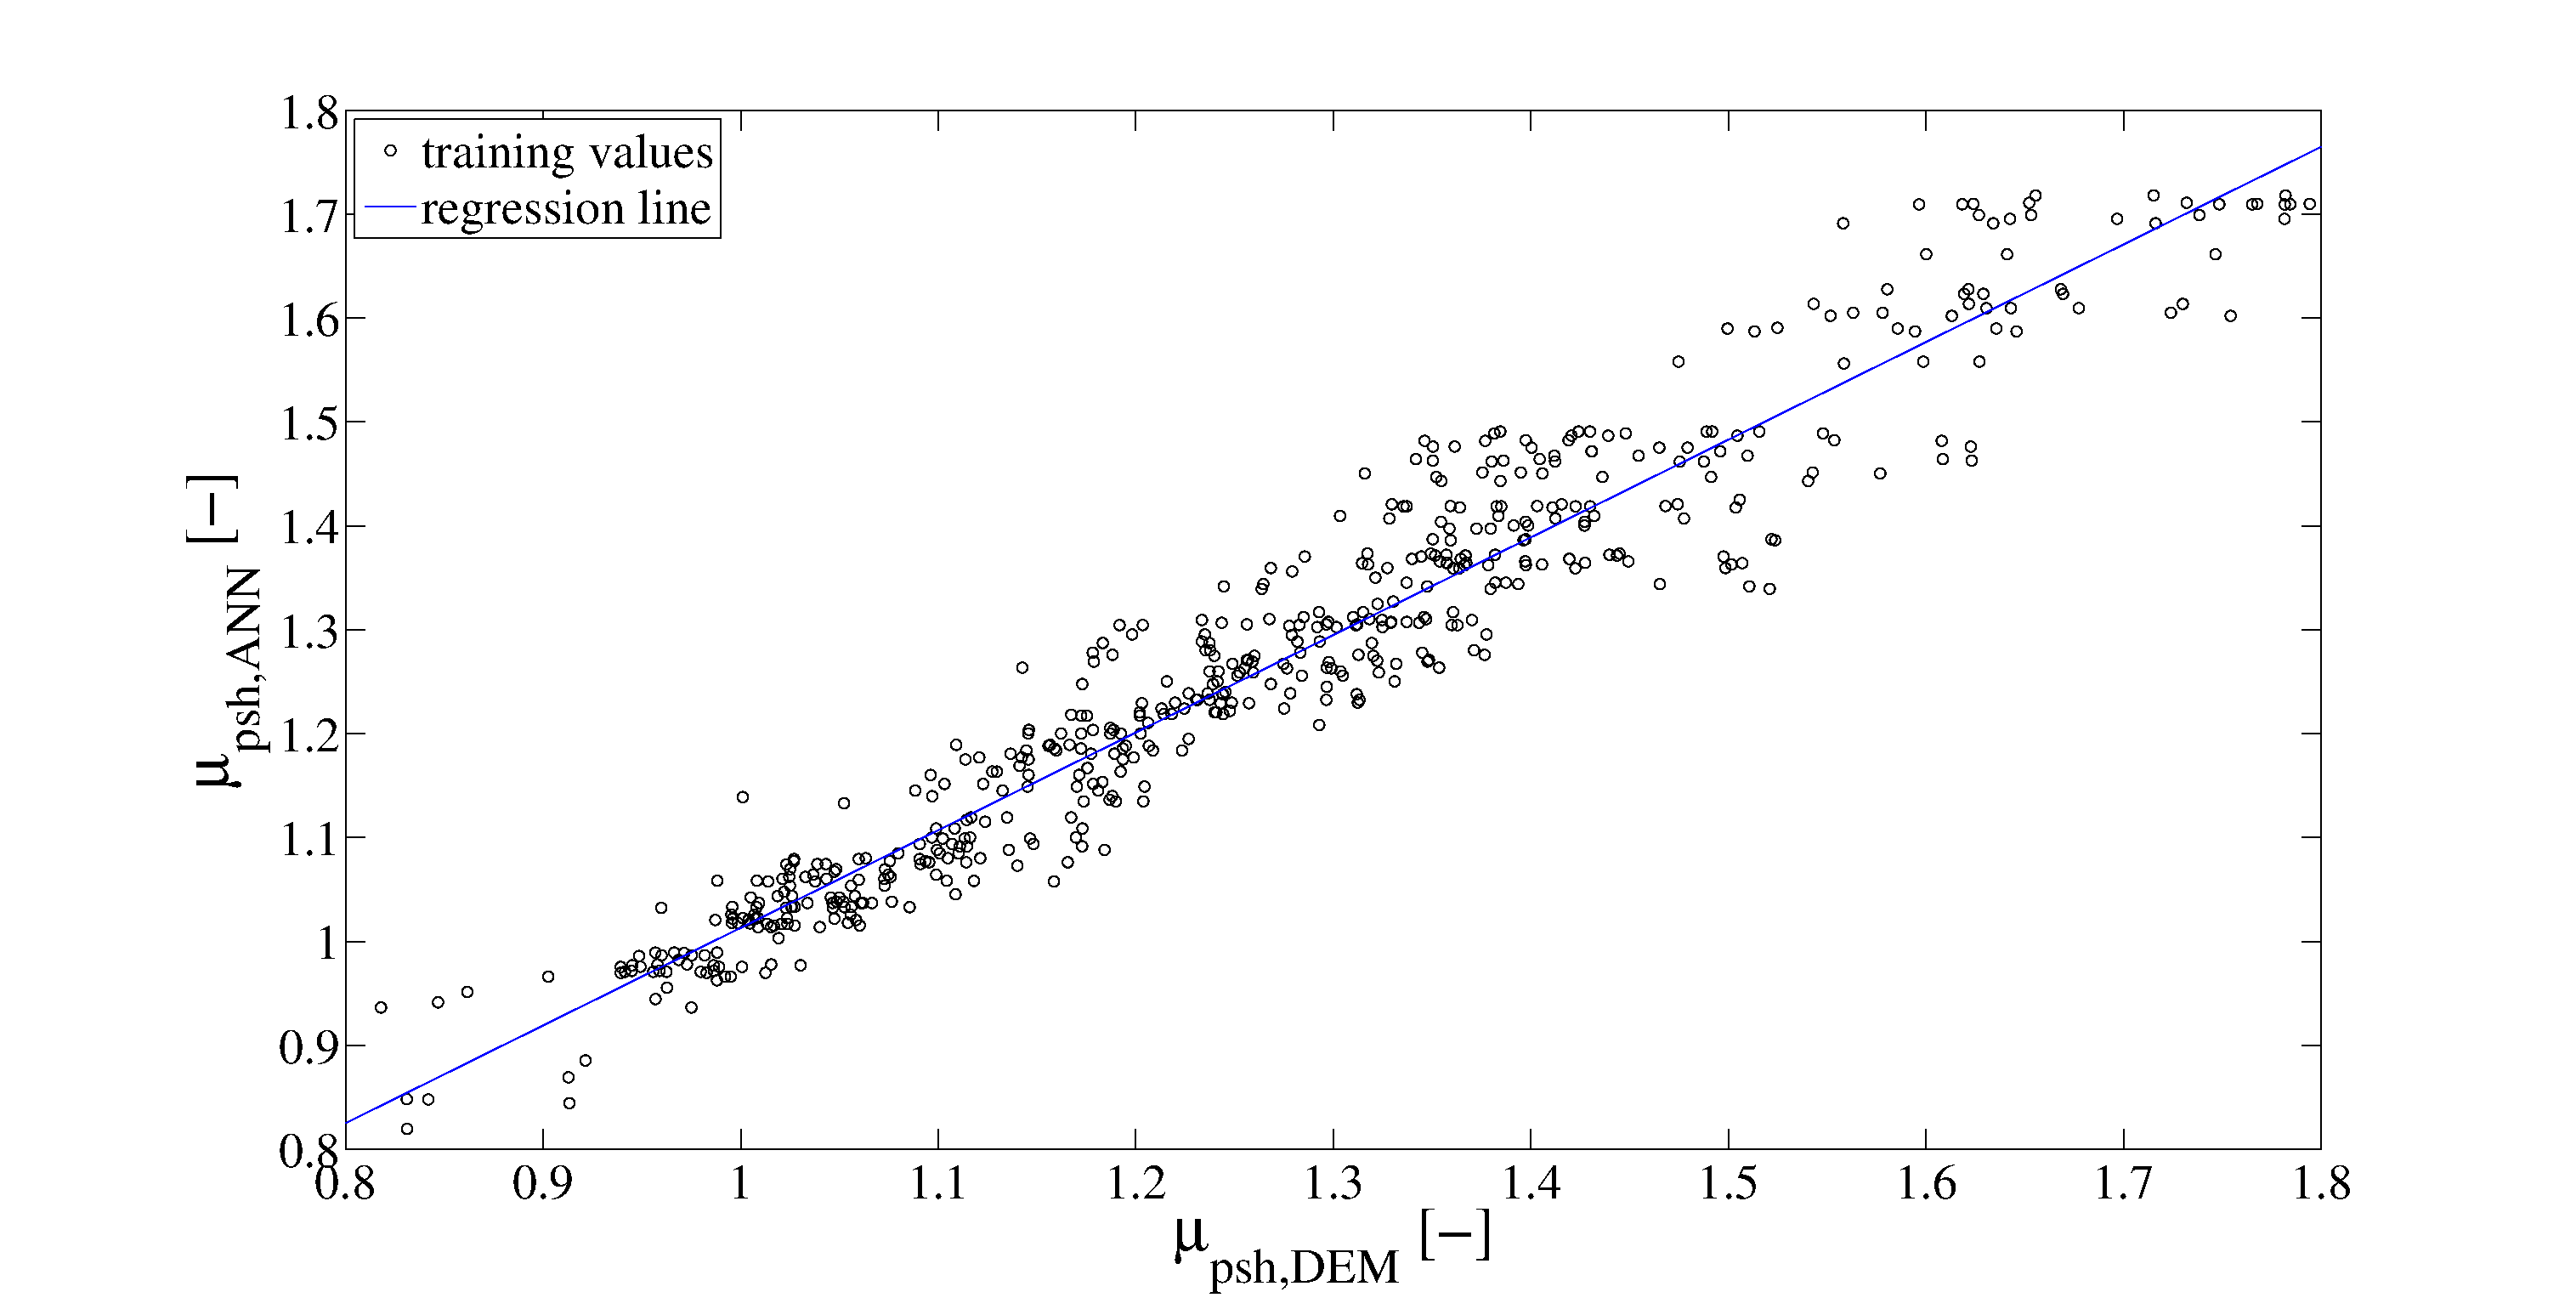
\includegraphics[width=.80\columnwidth]{images/022regression.eps}
% %[width=.48\textwidth]
% \caption[Comparison between prediction of the trained ANN and full DEM
% simulation]{Comparison between prediction of the trained Artificial Neural
% Network (\acs{ANN}) and 546 
% \wrong{write down all the simulations performed at the end.}
% full DEM simulations of the coefficient of pre-shear
% (\acs{mupsh}).}
% \label{fig:022regression} 
% \end{figure}

We checked \acs{r2}, \textit{mean absolute error}, 
\begin{equation}
MAE = \frac{\sum _{i=1}^{n} (x_{i}-\widehat{x}_{i})}{n} ,
\label{eq:meanAbsoluteError}
\end{equation}
\textit{mean squared error},
\begin{equation}
MSE = \frac{\sum _{i=1}^{n} (x_{i}-\widehat{x}_{i})^{2}}{n}
\label{eq:meanSquareError}
\end{equation}
and \textit{root mean squared error},
\begin{equation}
RMSE = \sqrt{\frac{\sum _{i=1}^{n} (x_{i}-\widehat{x}_{i})^{2}}{n}}
\label{eq:rootMeanSquareError}
\end{equation}
for the \textit{Bayesian linear
regression}, the \textit{Gaussian nonlinear
regression}, and the
\textit{\acs{ANN} regression} to establish the most effective method.
All were trained with the same training set. 
For instance, a comparison of the \acs{r2} for the \acs{mupsh} can be see in 
Fig. \ref{fig:143sctregressions}.
In Fig. \ref{fig:144aorregressions} a similar comparison for the \acs{AoR} can
be found.\\
In fact, the check was performed for each method by comparing the
\acs{DEM} bulk values of the test set against the bulk values predicted by each method from the 
corresponding \acs{DEM} input values of the test set. \\
Table \ref{tab:15regressionvalues} shows a quantitative comparison between the
three methods for the \acs{mupsh}. 
\begin{table}[htbp]
  \centering

    \begin{tabular}{lccc}
    \hline
          & Bayesian & Gaussian & ANN \\
          \hline
    Coefficient of determination (\acs{r2}) & 0.86  & 0.843 & 0.959 \\
    Root mean squared error & 0.057 & 0.061 & 0.031 \\
    Mean absolute error & 0.042 & 0.038 & 0.025 \\
    Mean squared error & 0.003 & 0.004 & 0.001 \\
    \hline
    \end{tabular}%
      \caption{Regression methods quantitative comparison.}
  \label{tab:15regressionvalues}%
\end{table}%
%************************************************

\section{Parameter Identification}
\label{sec:parameteridentification}

Since \acs{mupsh}, \acs{mush} and \acs{rhob} belonged to the shear-cell
simulations, their \acs{ANNs} were handled together: we had one cluster with three 
\acs{ANNs} for the shear cell and one with only one \acs{ANN} for the \acs{AoR}.
We could then proceed in identifying valid input parameters.

\subsection{Computational Condiderations}
\label{subsec:computationalcondiderations}

\citet{RefWorks:116, RefWorks:160} suggested using a Design of Experiments
(\acs{DoE}) method to determine the parameter combinations to be simulated.
They stated that this approach allows optimization of computation time
with an acceptable loss of precision.
The speed of the trained \acs{ANNs} enabled us to follow a different approach to
maximizing the precision of the characterization.\\

\begin{table}[h]
\centering
\begin{tabular}{lcccc}
\hline
 &  \ac{mus} & \ac{mur} & \ac{CoR} & \ac{rhop}  \\
  &	$[-]$  & $[-]$   & $[-]$   & $[kg/m3]$ \\
          \hline
    range & $[0.1 \ldots 1.0]$ & $[0.1 \ldots 1.0]$ & $[0.5 \ldots 0.9]$ &
    $[2000 \ldots 3500]$     \\
    \# rnd & 100   & 100   & 25    & 25    \\

\hline
\end{tabular}
\caption[DEM random input values]{DEM random input values. Within each range \#
random values are chosen.}
\label{tab:12DEMRandominputvalues}
\end{table}

\subsection{Decisional Limits}
\label{subsec:decisionallimits}

We created random values
in the range and numbers defined in Table \ref{tab:12DEMRandominputvalues}
according to a standard uniform distribution.
These combinations were then fed to and processed by the selected
\acs{ANNs}, and thus three bulk values for the shear
cell and one for the \acs{AoR} were obtained.
The \acs{ANN} evaluation was significantly faster than the \acs{DEM} simulations. The
individuation of the numerical bulk behaviours for all the \acs{DEM} combinations
did not take more than a few seconds on a single core.\\
\begin{figure}[!htb] 
\centering 
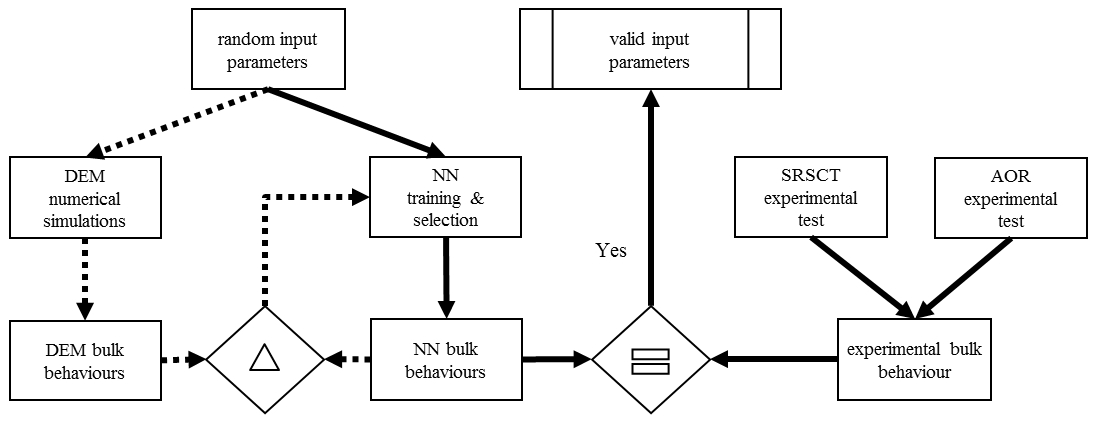
\includegraphics[width=.96\textwidth]{images/019methodology} 
\caption[Method]{Method. In the training phase (dashed lines)
$DEM$ simulations are performed
with random initial input parameters.
The behaviours obtained are used to train the
Artificial Neural Networks ($ANNs$) in a loop that continues until the
difference between the outputs of each $ANN$ and its simulations is below the
limit ($\Delta$).
In the parameters identification phase (solid
lines) we identify valid input parameters by comparing (\textbf{=}) $ANNs$ and
experimental behaviours.}
\label{fig:019methodology} 
\end{figure}
As can be seen in Fig. \ref{fig:019methodology}, in the parameters
identification phase (solid lines) we identify valid input parameters by comparing (\textbf{=}) \acs{ANNs} and
experimental behaviours.\\
We obtained for each of the twelve load conditions of the \acs{SCT} three bulk
values (\acs{mupsh}, \acs{mush} and \acs{rhob}).
The fourth bulk value was the result of two angle of repose (\acs{AoR}) tests that
recreated the repose angle observed in a pile of the
real material. 
Subsequently, we compared the \acs{ANN} and experimental bulk behaviours for the
twelve shear-cell load conditions.
If in a DEM-parameter combination all the three bulk values differed by less 
than 5\% from those of the corresponding experiments, i.e.:
%************************************************
\begin{equation}
 \begin{cases}
\text{if } & \lvert{1-\frac{\mu_{psh,num}}{\mu_{psh,exp}}}\rvert < 5\%  ,\\
\text{and if } & \lvert{1-\frac{\mu_{sh,num}}{\mu_{sh,exp}}}\rvert < 5\% , \\ 
\text{and if } & \lvert{1-\frac{\rho_{p,num}}{\rho_{p,exp}}}\rvert < 5\% ,\\ 
\end{cases}
 \label{eq:check2}
\end{equation}
the combination was marked. The marked combinations were processed by the
\acs{AoR} \acs{ANN}, and then compared with the experiment.
Were considered valid those that differed by less than $5\%$ also in this
comparison (Eq. \ref{eq:checkaor}):
%************************************************
\begin{equation}
\text{if} ~~~~~~ \lvert{1-\frac{AoR_{num}}{AoR_{exp}}}\rvert < 5\% .
\label{eq:checkaor}
\end{equation}
%************************************************

\subsection{Value representation}
\label{subsec:valuerepresentation}

We decided to show the valid values achieved through the procedure with three
compact graphical schemes:

\begin{itemize}
  \item{parameter space plot,}
  \item{box plot,}
  \item{density plot.}
\end{itemize}

\subsubsection{Parameter space plot}
\label{subsubsec:parameterspaceplot}

An example of a parameter space plot can be seen
in Fig. \ref{fig:041radarpirker1schulze1068}.
On the axes we can see:
\begin{itemize}
  \item{the \acl{CoR} (\acs{CoR}),}
  \item{the \acl{mus} (\acs{mus}),}
  \item{the \acl{mur} (\acs{mur}),}  
  \item{the \acl{rhob} (\acs{rhob}).}
\end{itemize}
Further, are shown:
\begin{itemize}
  \item{the minimum input values amongst the millions possible combinations,
  with a blue straight line;}
  \item{the minimum values amongst the valid, or marked combinations, with a
  green straight line;}
  \item{the mean values amongst the valid, or marked combinations, with an
  orange dotted line;}
  \item{the negative standard deviations from the mean values amongst the valid,
  or marked combinations, with a red straight line;}
  \item{the positive standard deviations from the mean values amongst the valid,
  or marked combinations, with a red straight line;}  
  \item{the maximum values amongst the valid, or marked combinations, with a
  green straight line;}
  \item{the maximum input values amongst the millions possible combinations,
  with a blue straight line.}  
\end{itemize}

The shaded area indicates valid parameter combinations, and dark shaded
values indicate the confidence range.
This plot is especially interesting for reliability consideration, see Section
\ref{subsec:reliabilityconsiderations}.

\begin{figure}[htbp]
	\centering

    \subfloat[Parameter space plot, \acs{SCT}, $\sigma_n=1068$ Pa, P=0.8.]{
	  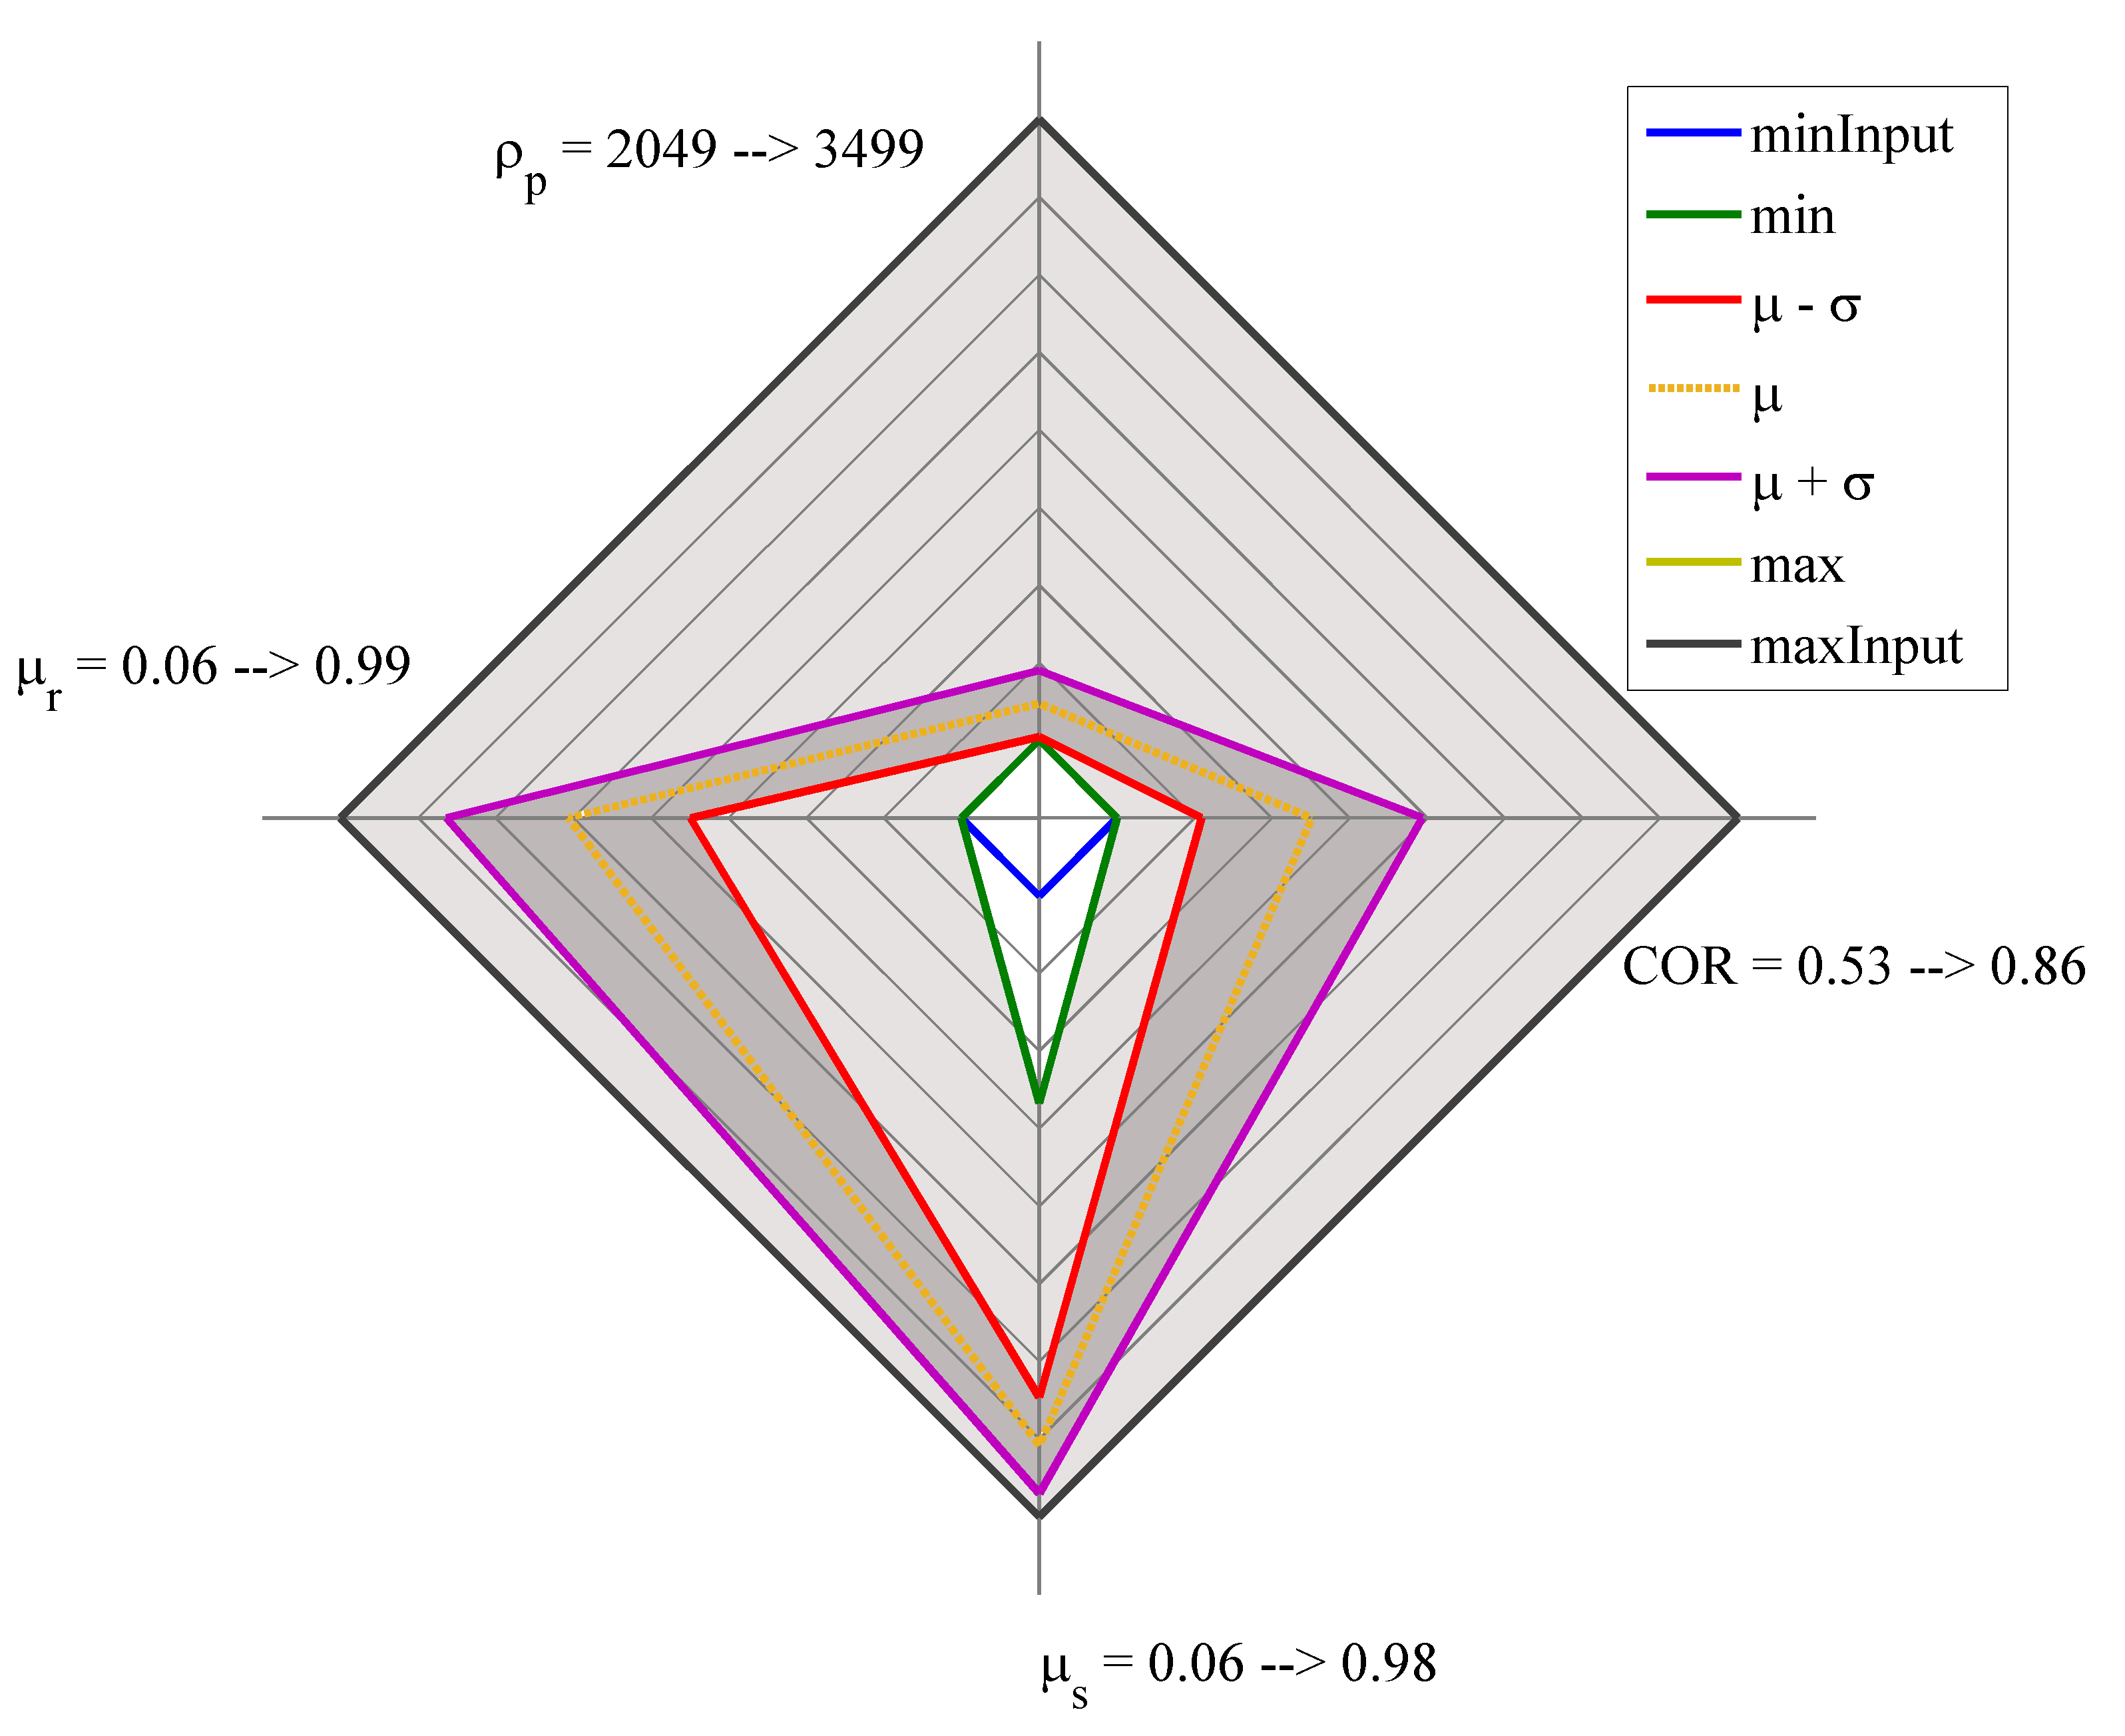
\includegraphics[width=.5\columnwidth]{images/150ParamSpaceSCT1068p08sinterfine}
	  \label{fig:150ParamSpaceSCT1068p08sinterfine}  }
	 
    \subfloat[Parameter space plot, \acs{SCT}, $\sigma_n=1068$ Pa, P=1.0.]{
	  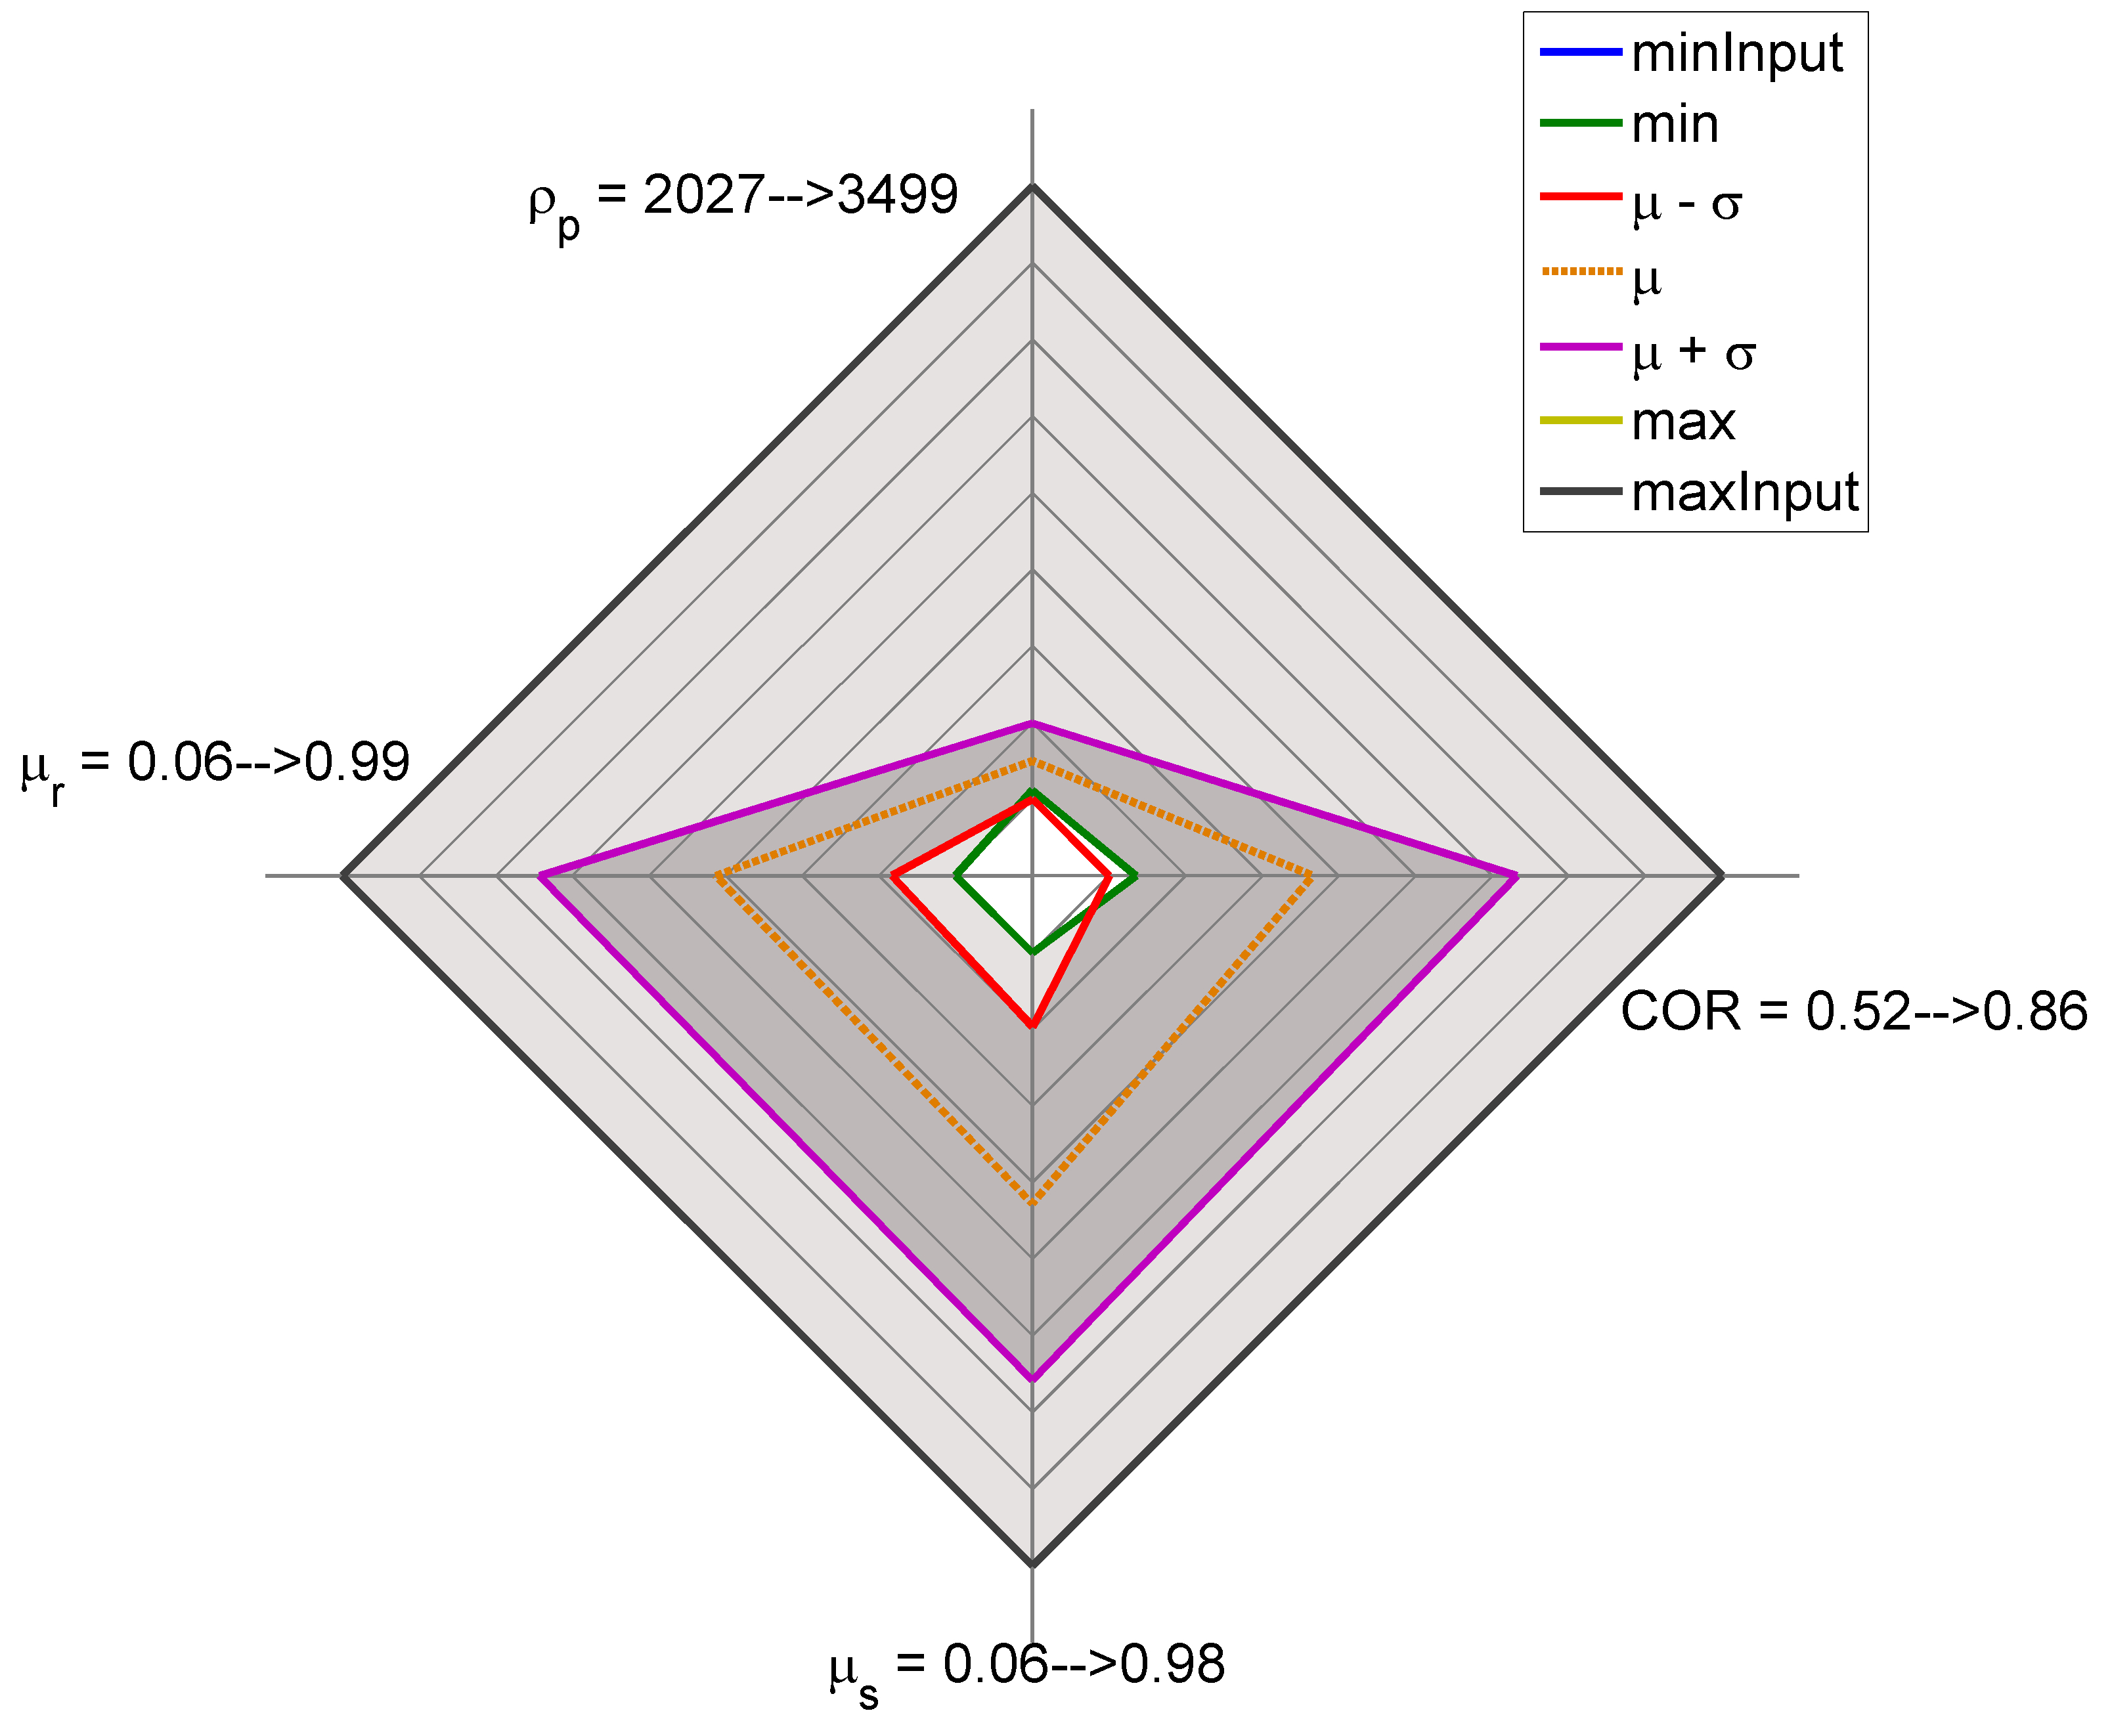
\includegraphics[width=.5\columnwidth]{images/041radarpirker1schulze1068}
	  \label{fig:041radarpirker1schulze1068}  } 
	  
    \subfloat[Parameter space plot, \acs{SCT}, $\sigma_n=1068$ Pa, P=1.2.]{
	  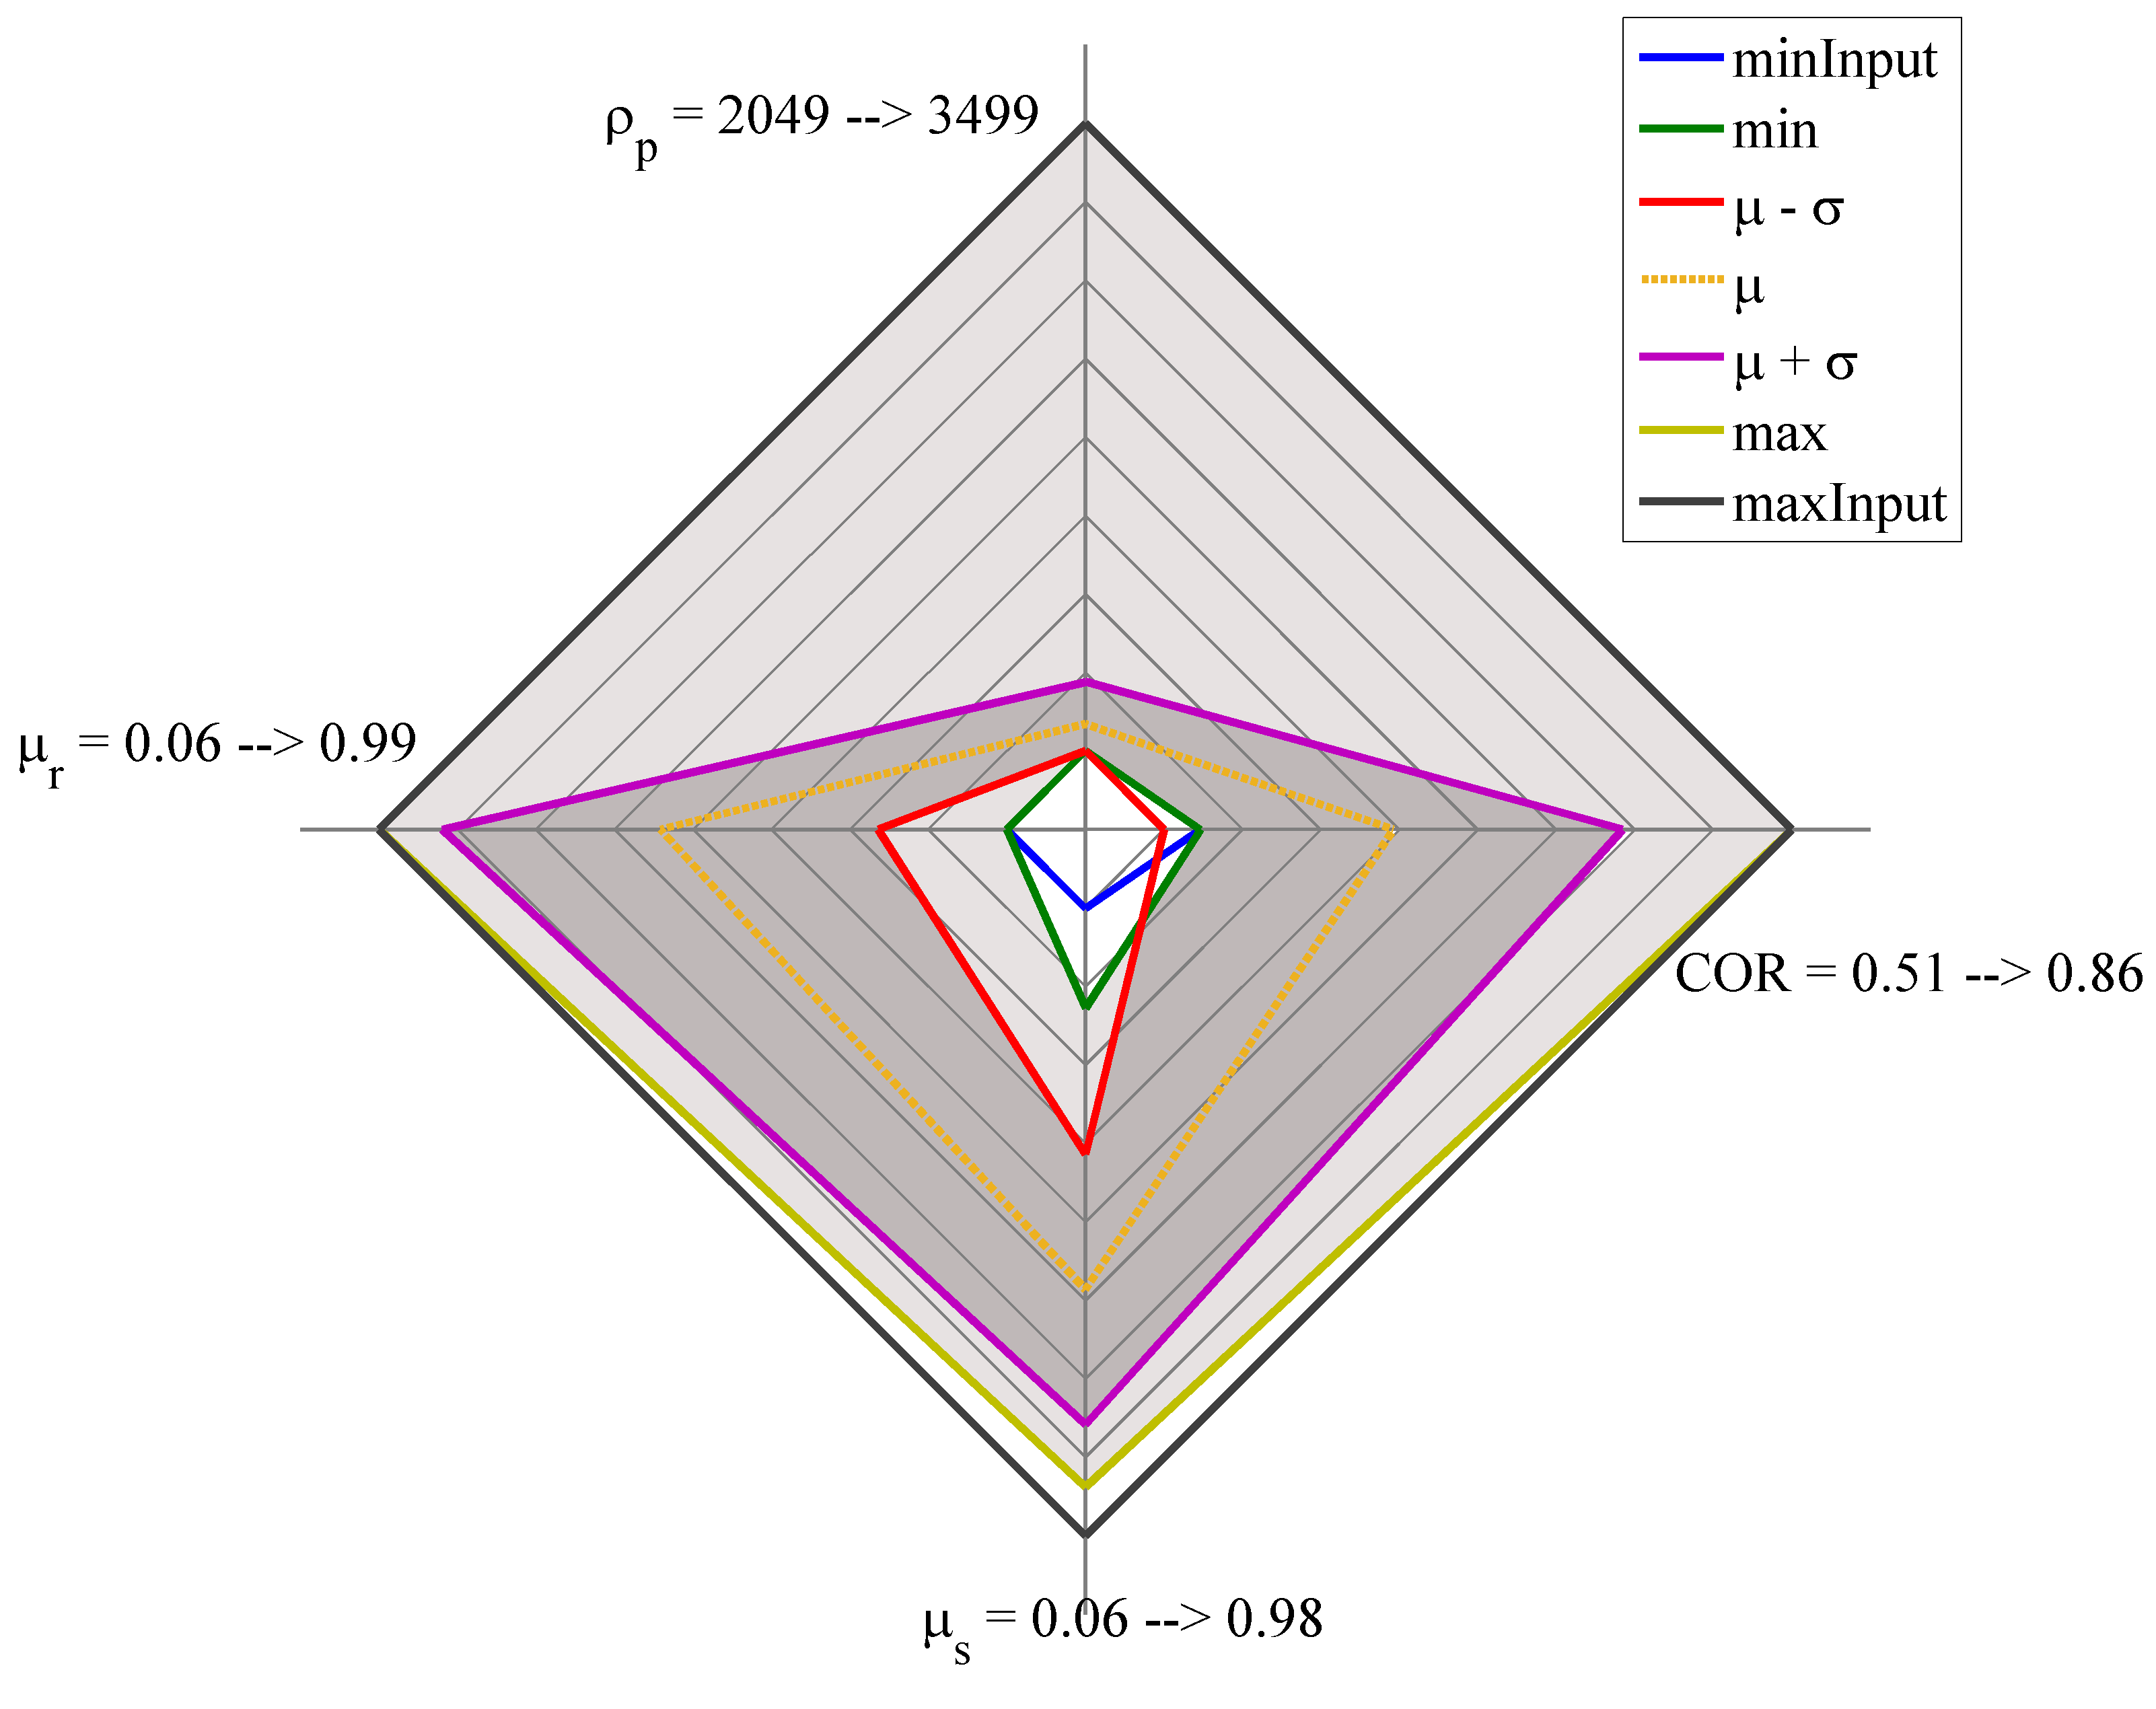
\includegraphics[width=.5\columnwidth]{images/151ParamSpaceSCT1068p12sinterfine}
	  \label{fig:151ParamSpaceSCT1068p12sinterfine}  } 	  
	  

 % \hfill\null
  \caption[SCT parameter space plots 1]{SCT parameter space
  plots for sinter fine, $\sigma_n=1068$ Pa.}
  \label{fig:149paramspaceplotsct1068}
\end{figure}

% \begin{figure}%[!h] 
% \centering 
% 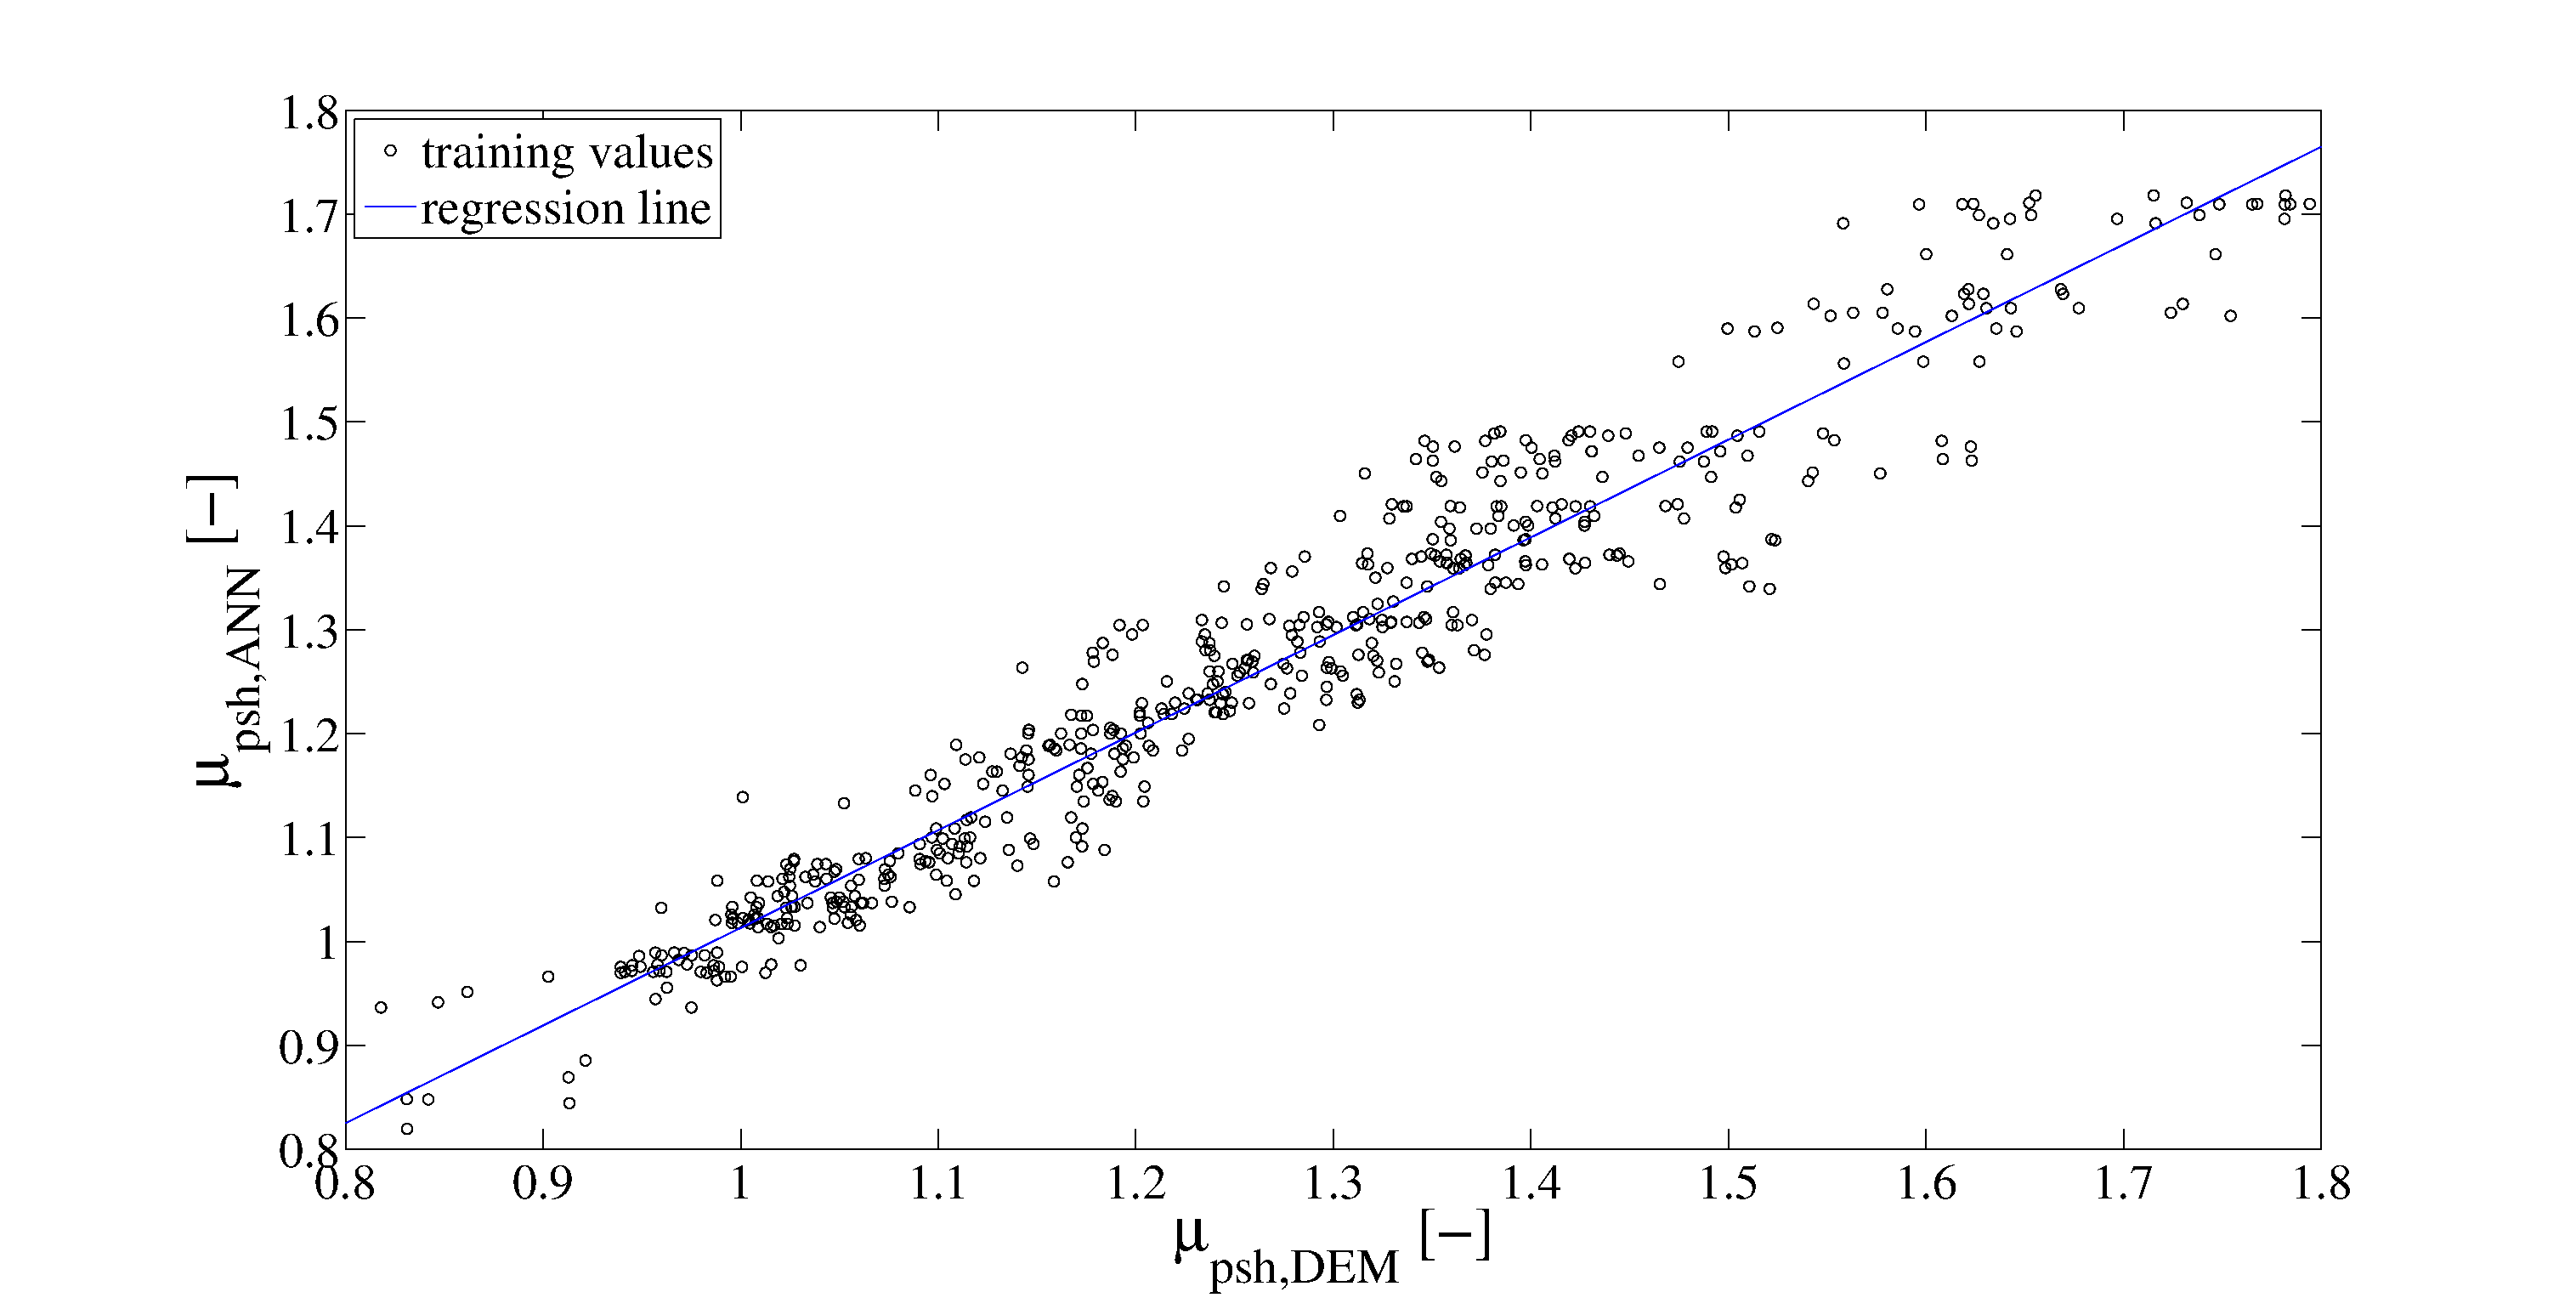
\includegraphics[width=.80\columnwidth]{images/022regression.eps}
% %[width=.48\textwidth]
% \caption[Comparison between prediction of the trained ANN and full DEM
% simulation]{Comparison between prediction of the trained Artificial Neural
% Network (\acs{ANN}) and 546 
% \wrong{write down all the simulations performed at the end.}
% full DEM simulations of the coefficient of pre-shear
% (\acs{mupsh}).}
% \label{fig:022regression} 
% \end{figure}


\subsubsection{Box plot}
\label{subsubsec:boxplot}
  
An example of a box plot can be seen
in Fig. \ref{fig:145BoxSCT1068p08sinterfine}.
\citet{RefWorks:207} defines a box plot a graphical representation of
collections of numerical data by means of their quartiles.
These are three points, which divide the data in four groups that are equals and
contain a quarter of the data each.\\
In a box plot the values between the first quartile (25\%) and the third
quartile (75\%) are included in a blue box.
Further, so called \textit{baffles} or \textit{whishers} are lines, which are
extended as far as the minimum and maximum values.
Finally, the median is represented as a red straight line.
Values are normalized, meaning that for each input value the maximum extracted
is one.

\begin{figure}[htbp]
	\centering

    \subfloat[Box plot, \acs{SCT}, $\sigma_n=1068$ Pa, P=0.8.]{
	  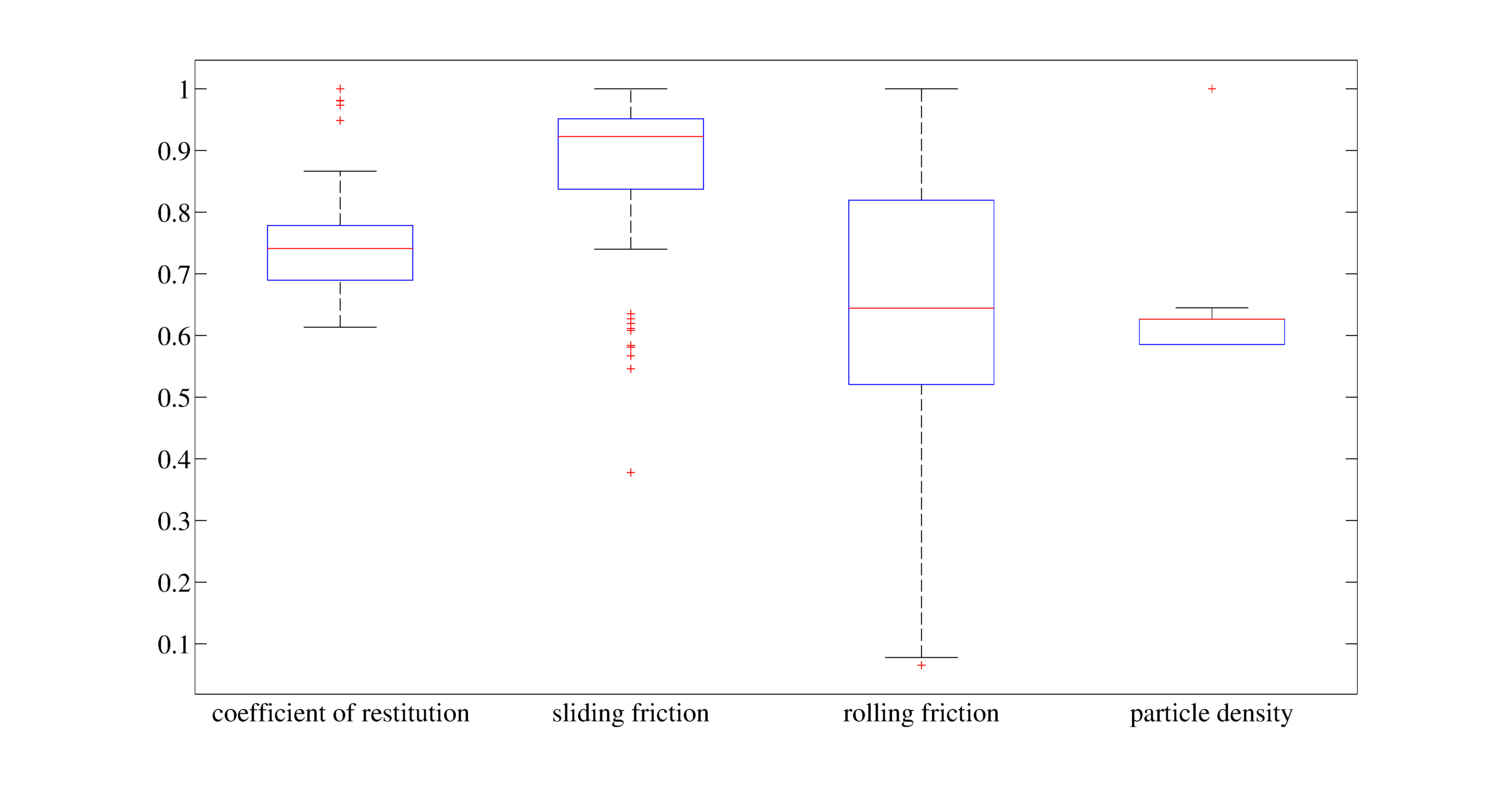
\includegraphics[width=.75\columnwidth]{images/145BoxSCT1068p08sinterfine}
	  \label{fig:145BoxSCT1068p08sinterfine}  }
	 
    \subfloat[Box plot, \acs{SCT}, $\sigma_n=1068$ Pa, P=1.0.]{
	  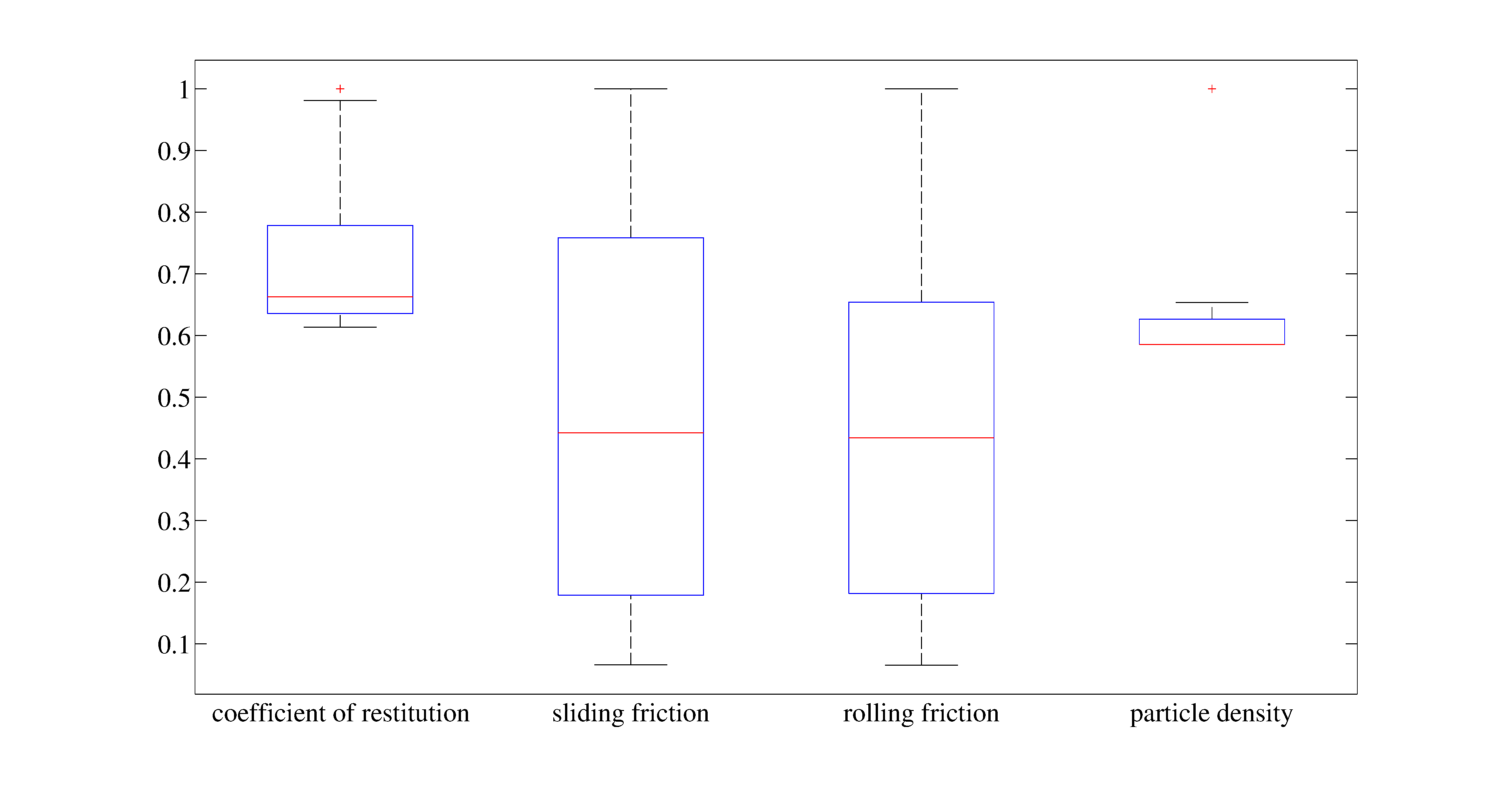
\includegraphics[width=.75\columnwidth]{images/148BoxSCT1068p10sinterfine}
	  \label{fig:147BoxSCT1068p10sinterfine}  } 
	  
    \subfloat[Box plot, \acs{SCT}, $\sigma_n=1068$ Pa, P=1.2.]{
	  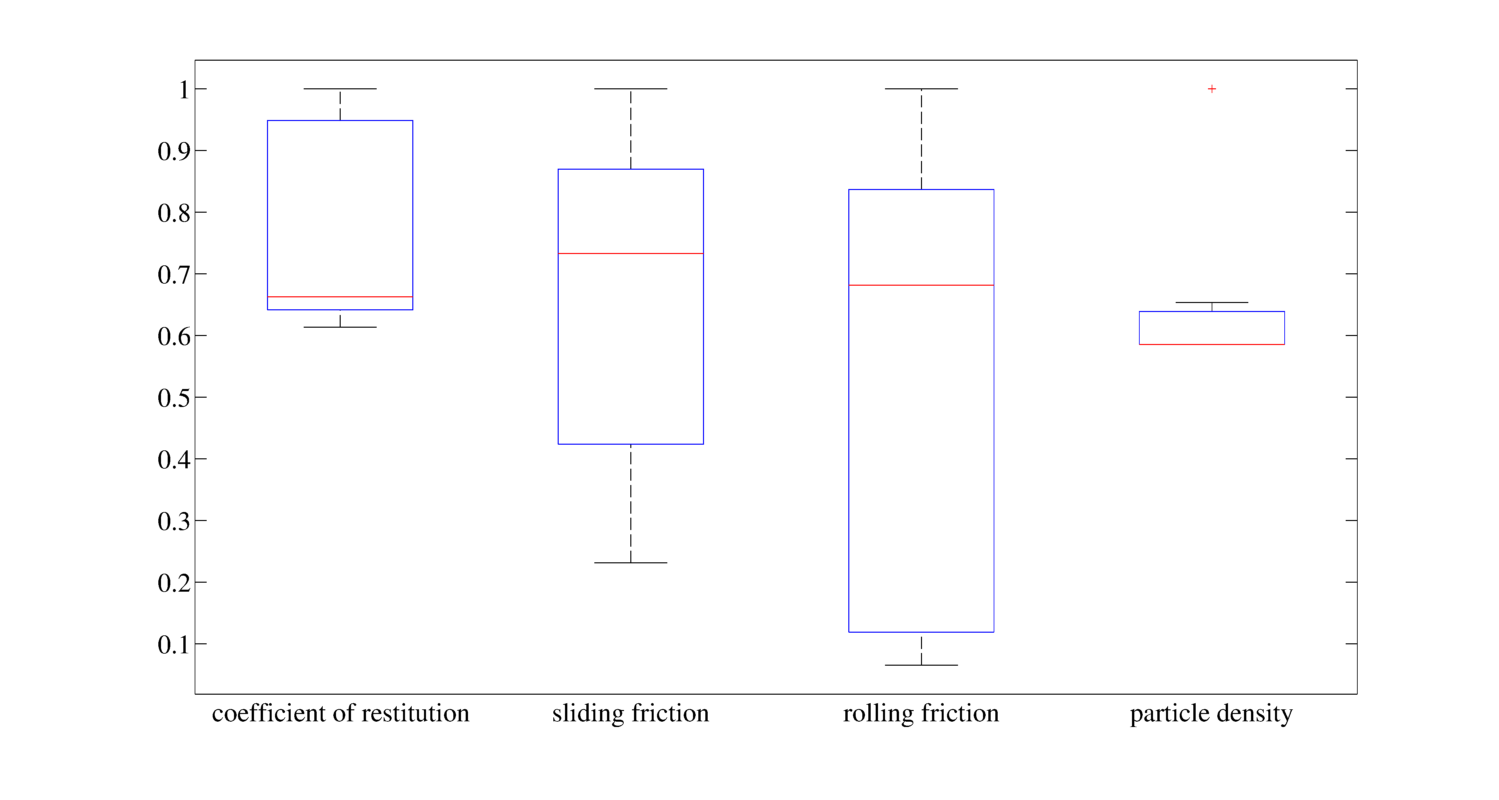
\includegraphics[width=.75\columnwidth]{images/147BoxSCT1068p12sinterfine}
	  \label{fig:148BoxSCT1068p12sinterfine}  } 	  
	  

 % \hfill\null
  \caption[SCT box plots 1]{SCT box
  plots for sinter fine, $\sigma_n=1068$ Pa.}
  \label{fig:146boxplotsct1068}
\end{figure}

% \begin{figure}%[!h] 
% \centering 
% 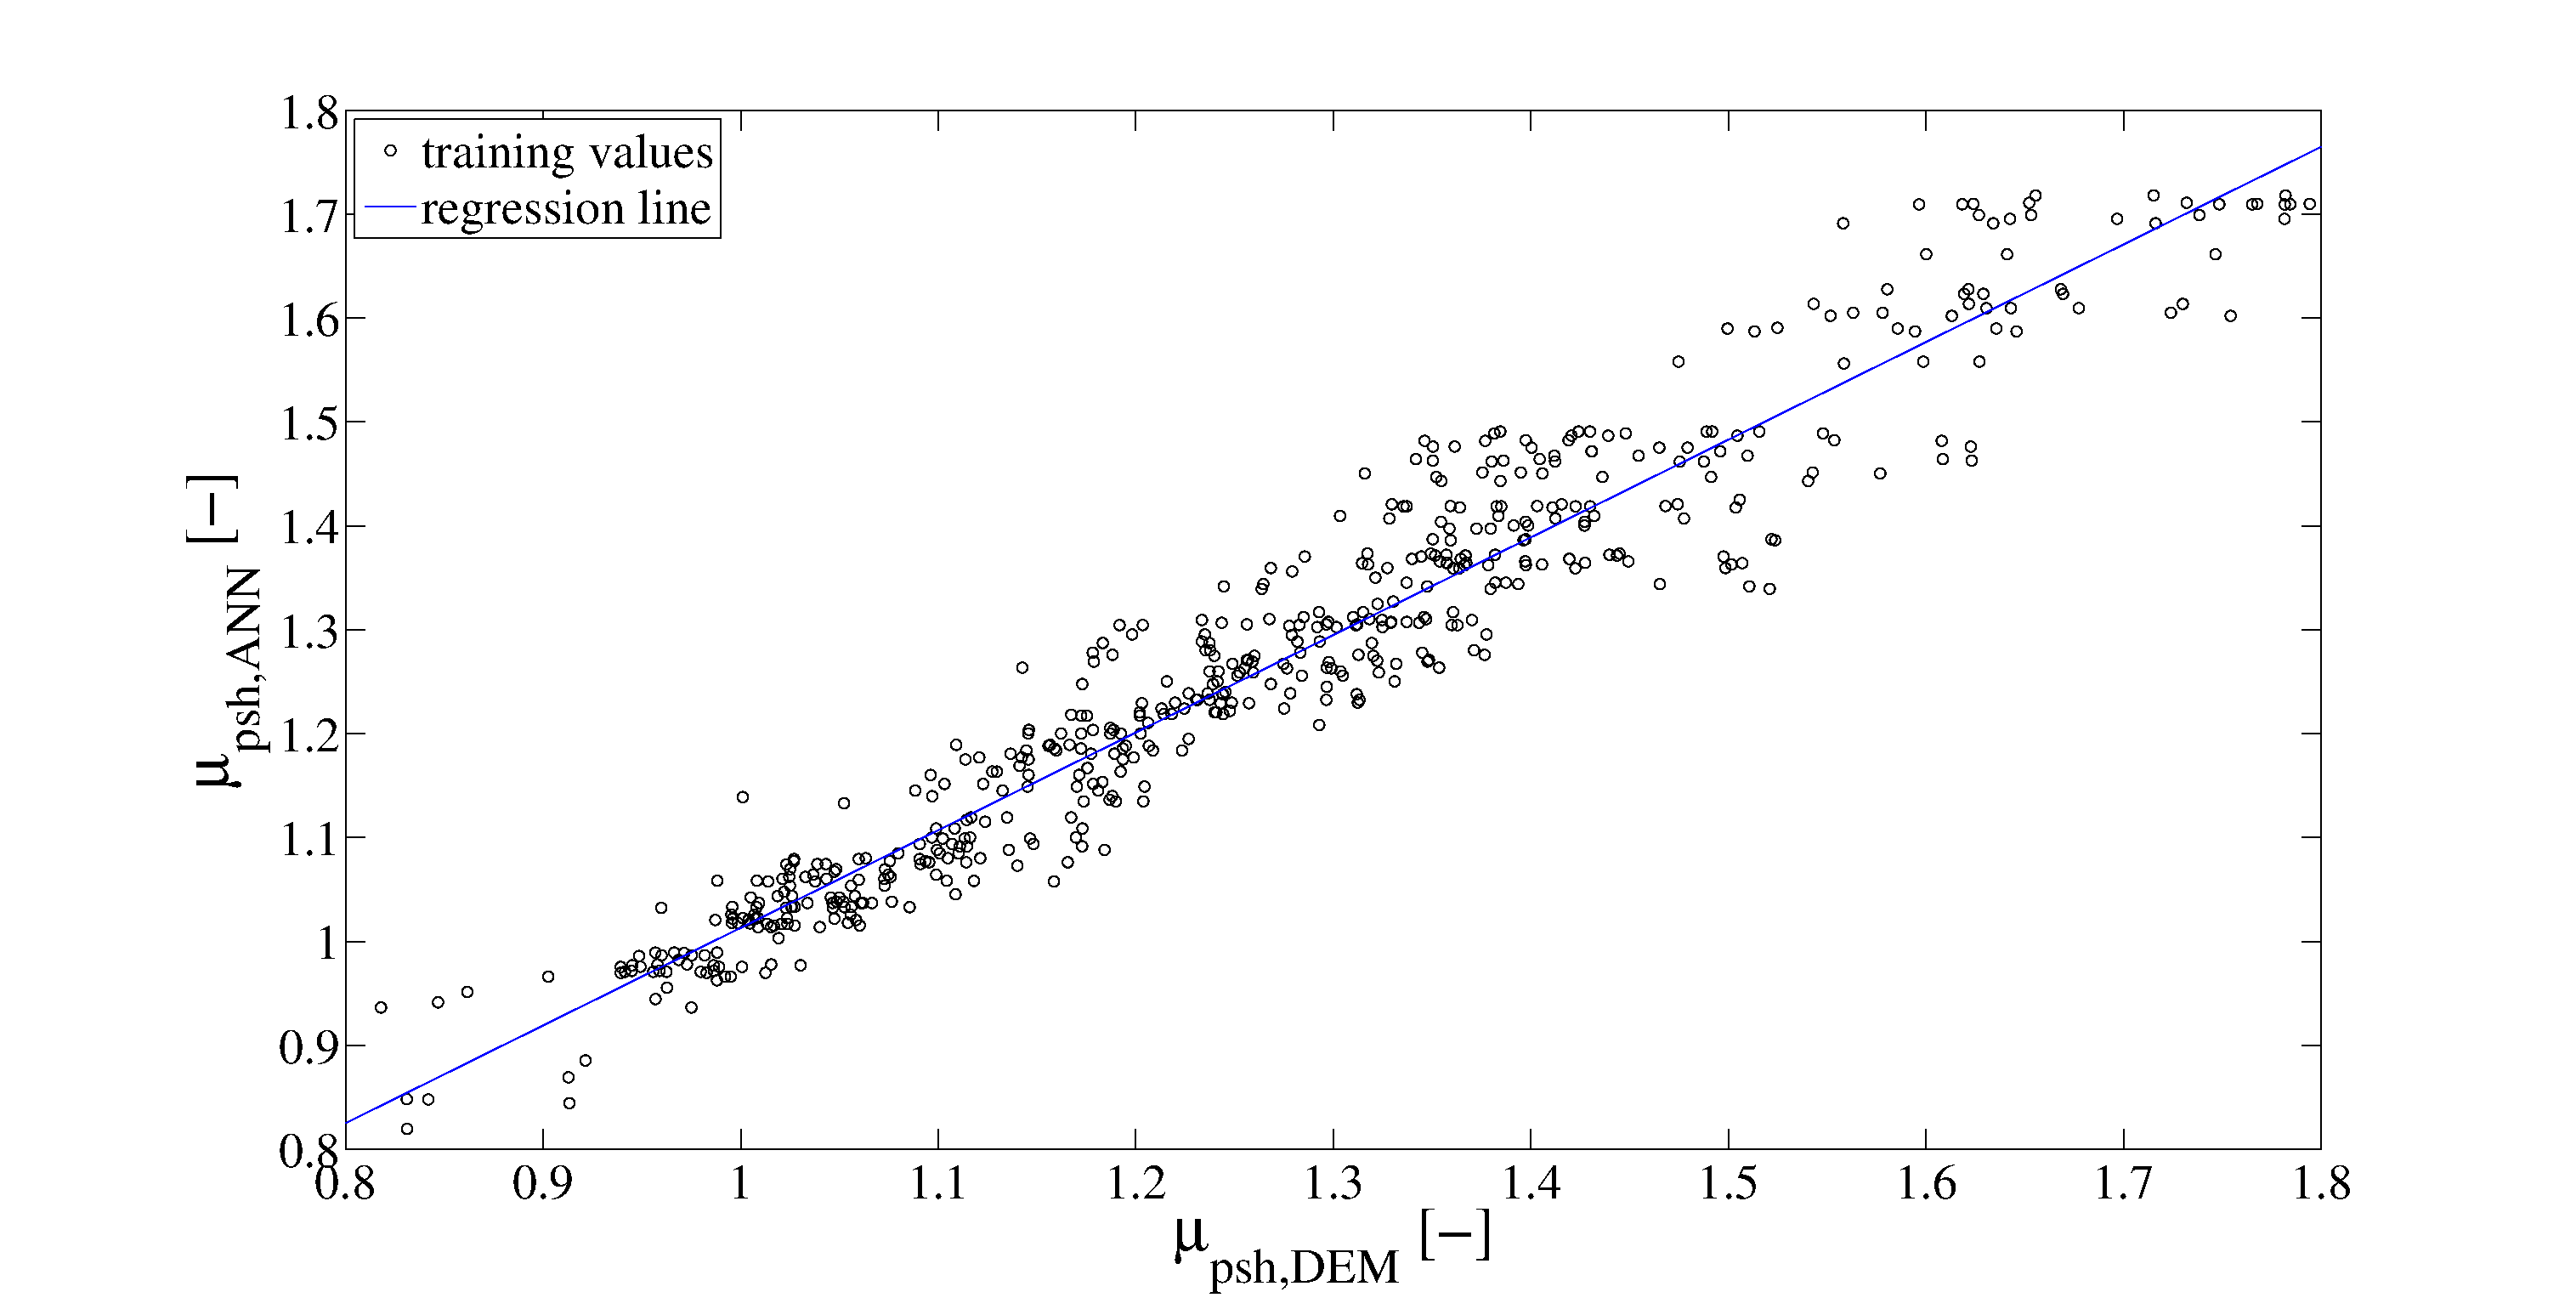
\includegraphics[width=.80\columnwidth]{images/022regression.eps}
% %[width=.48\textwidth]
% \caption[Comparison between prediction of the trained ANN and full DEM
% simulation]{Comparison between prediction of the trained Artificial Neural
% Network (\acs{ANN}) and 546 
% \wrong{write down all the simulations performed at the end.}
% full DEM simulations of the coefficient of pre-shear
% (\acs{mupsh}).}
% \label{fig:022regression} 
% \end{figure}

\subsubsection{Density plot}
\label{subsubsec:densityplot}

Further, we observed that various \acs{DEM} parameter
combinations could reproduce the experimental behaviour, and thus evaluated
their mutual dependencies.
This is shown more clearly in a density plot (e.g., Fig. 
\ref{fig:152TileSCT1068p08sinterfine}) 
of the particles' coefficient of restitution (\acs{CoR}) in relation to
the coefficients of sliding friction (\acs{mus}) and rolling friction (\acs{mur}); 
in the white area, no valid sets of simulation parameters could be found.
In each cell the valid sets are grouped according to the 4 different COR
ranges.
Each cell is coloured according to the group with the most members.

\begin{figure}[htbp]
	\centering

    \subfloat[Density plot, \acs{SCT}, $\sigma_n=1068$ Pa, P=0.8.]{
	  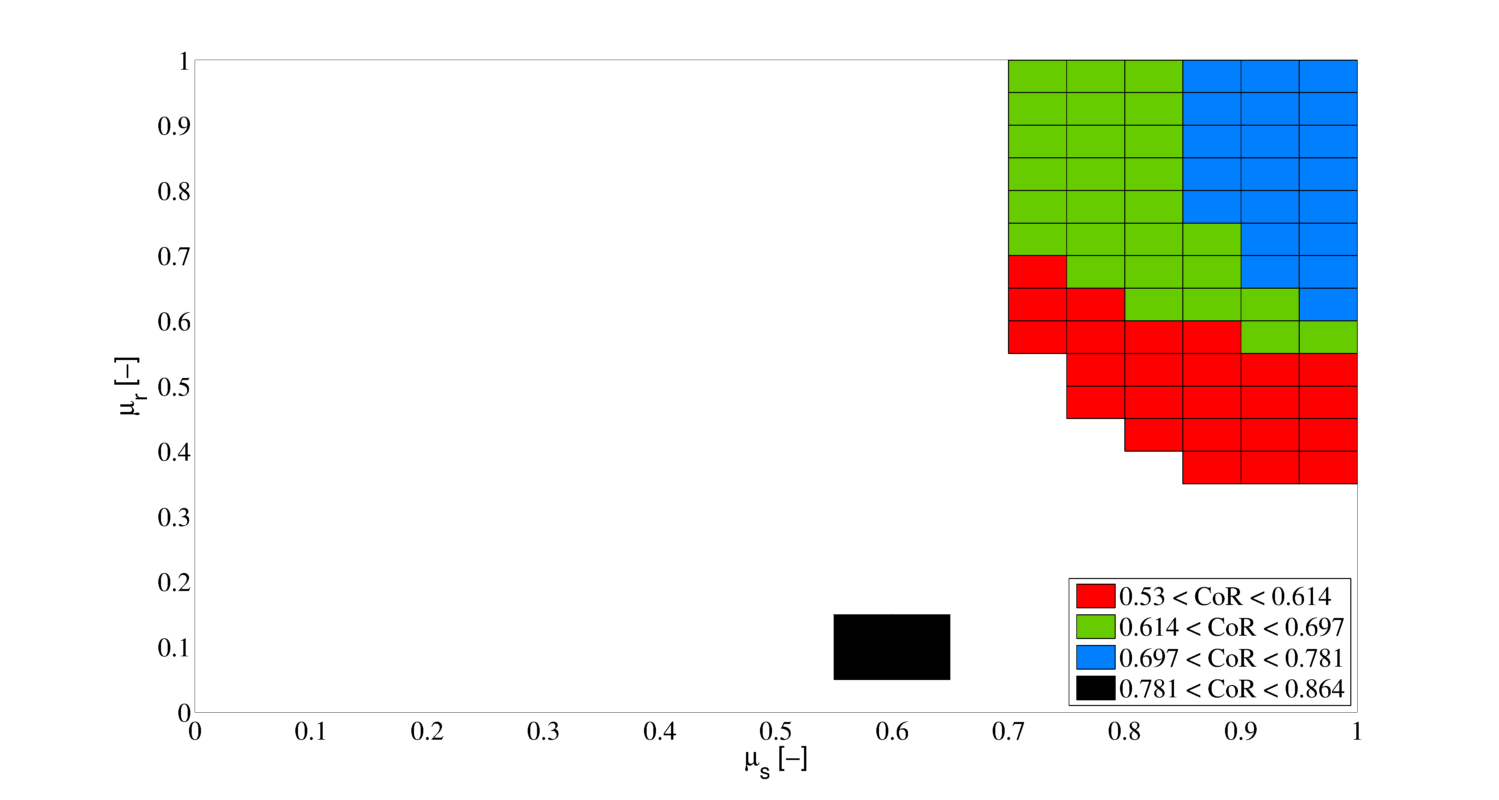
\includegraphics[width=.75\columnwidth]{images/152TileSCT1068p08sinterfine}
	  \label{fig:152TileSCT1068p08sinterfine}  }
	 
    \subfloat[Density plot, \acs{SCT}, $\sigma_n=1068$ Pa, P=1.0.]{
	  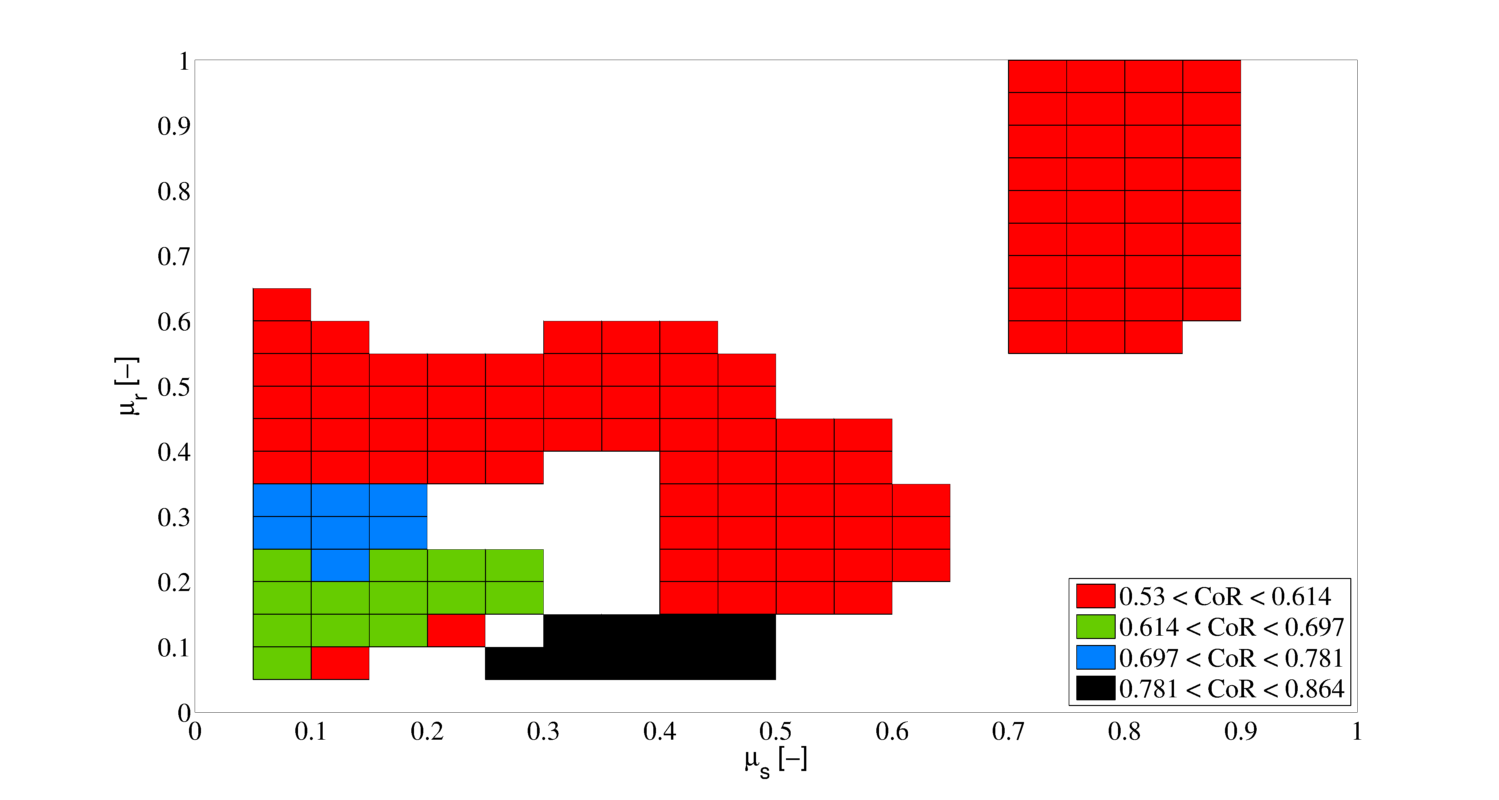
\includegraphics[width=.75\columnwidth]{images/153TileSCT1068p10sinterfine}
	  \label{fig:153TileSCT1068p10sinterfine}  } 
	  
    \subfloat[Density plot, \acs{SCT}, $\sigma_n=1068$ Pa, P=1.2.]{
	  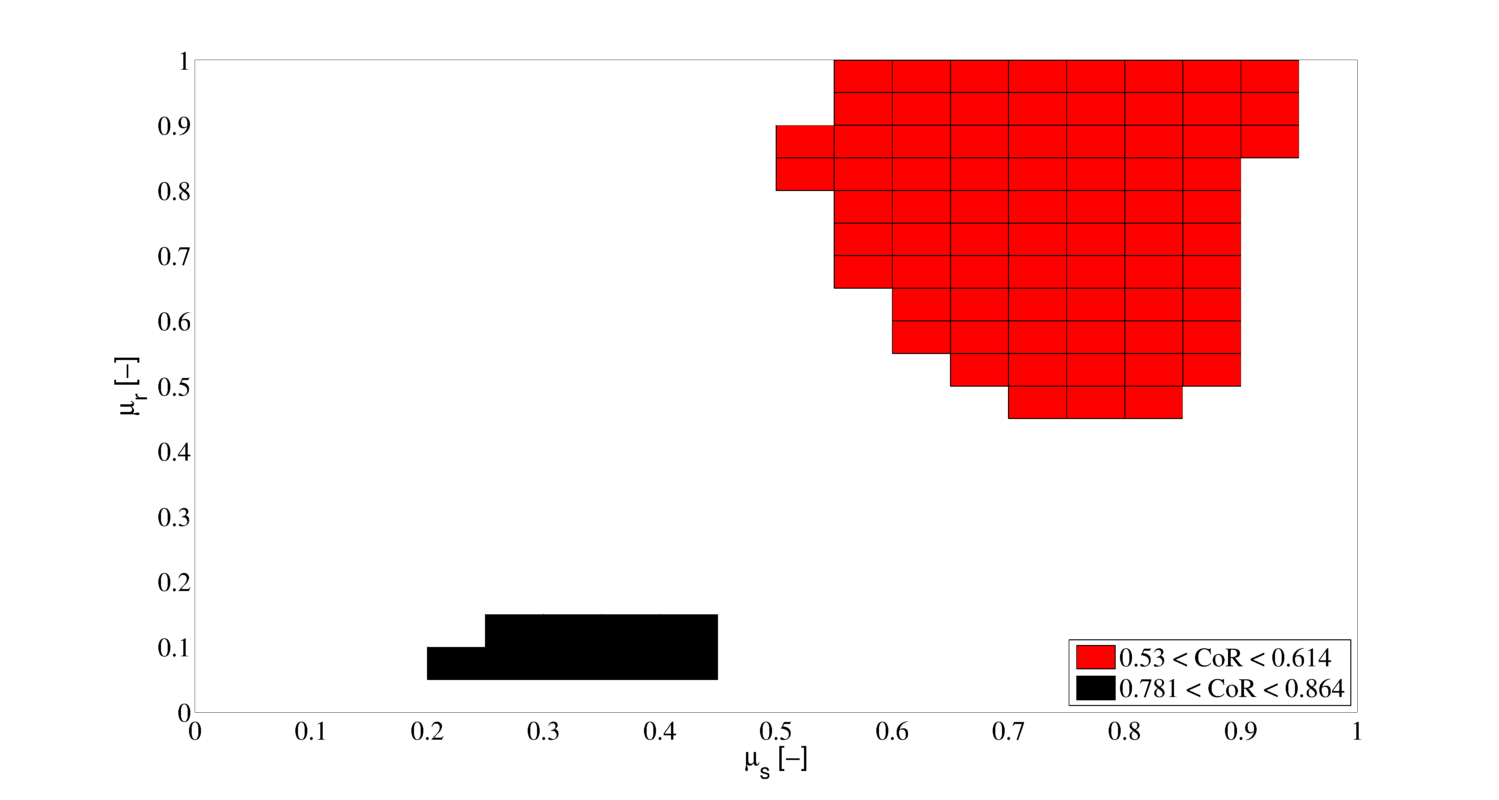
\includegraphics[width=.75\columnwidth]{images/154TileSCT1068p12sinterfine}
	  \label{fig:154TileSCT1068p12sinterfine}  } 	  
	  

 % \hfill\null
  \caption[SCT Density plots 1]{SCT Density
  plots for sinter fine, $\sigma_n=1068$ Pa.}
  \label{fig:155tileplotsct1068sinterfine}
\end{figure}

% \begin{figure}%[!h] 
% \centering 
% 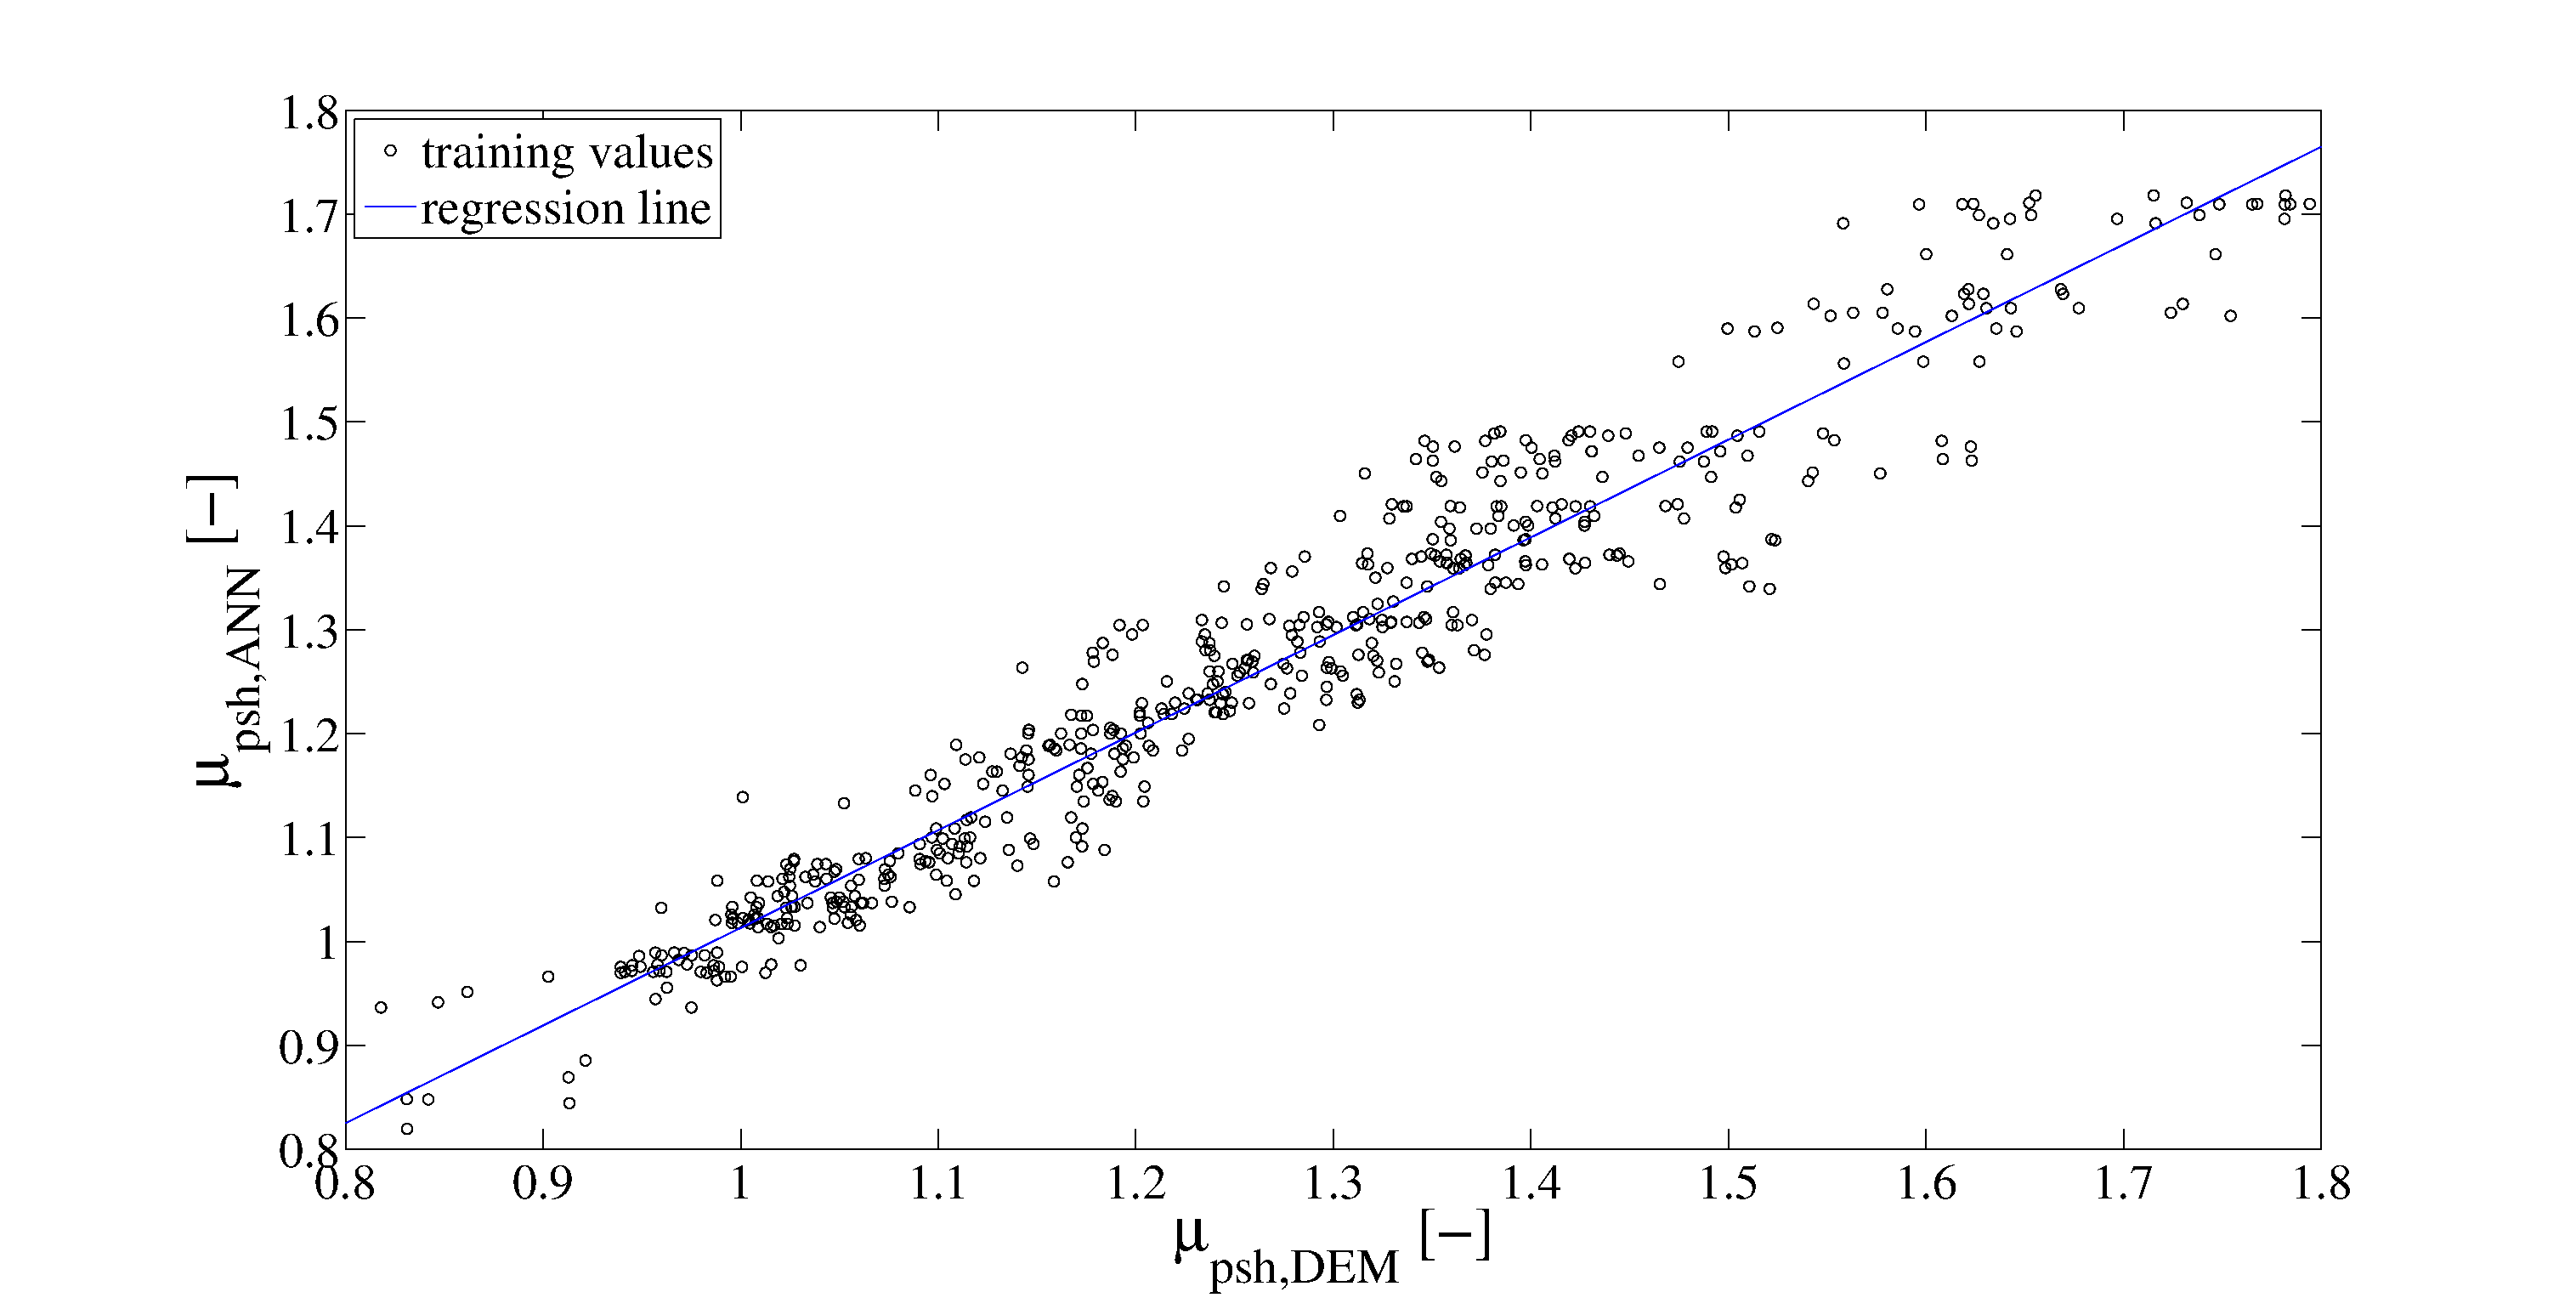
\includegraphics[width=.80\columnwidth]{images/022regression.eps}
% %[width=.48\textwidth]
% \caption[Comparison between prediction of the trained ANN and full DEM
% simulation]{Comparison between prediction of the trained Artificial Neural
% Network (\acs{ANN}) and 546 
% \wrong{write down all the simulations performed at the end.}
% full DEM simulations of the coefficient of pre-shear
% (\acs{mupsh}).}
% \label{fig:022regression} 
% \end{figure}

%************************************************
%************************************************

\section{Sinter fine Characterization}
\label{sec:sinterfinecharacterization}

We realized 6,250,000 parameter of combinations random values for sinter fine.
Amongst them we searched for values complying with the experimental results.
Further, we investigated the reliability of the procedure, see Section
\ref{subsec:reliabilityconsiderations}.

\subsection{SCT parameter space plot for Sinter fine}
\label{subsec:sctparameterspacesinterfine}

\begin{figure}[htbp]
\centering 
  \subfloat[Parameter space plot, \acs{SCT}, $\sigma_n=1068$ Pa, P=1.0.]{
	  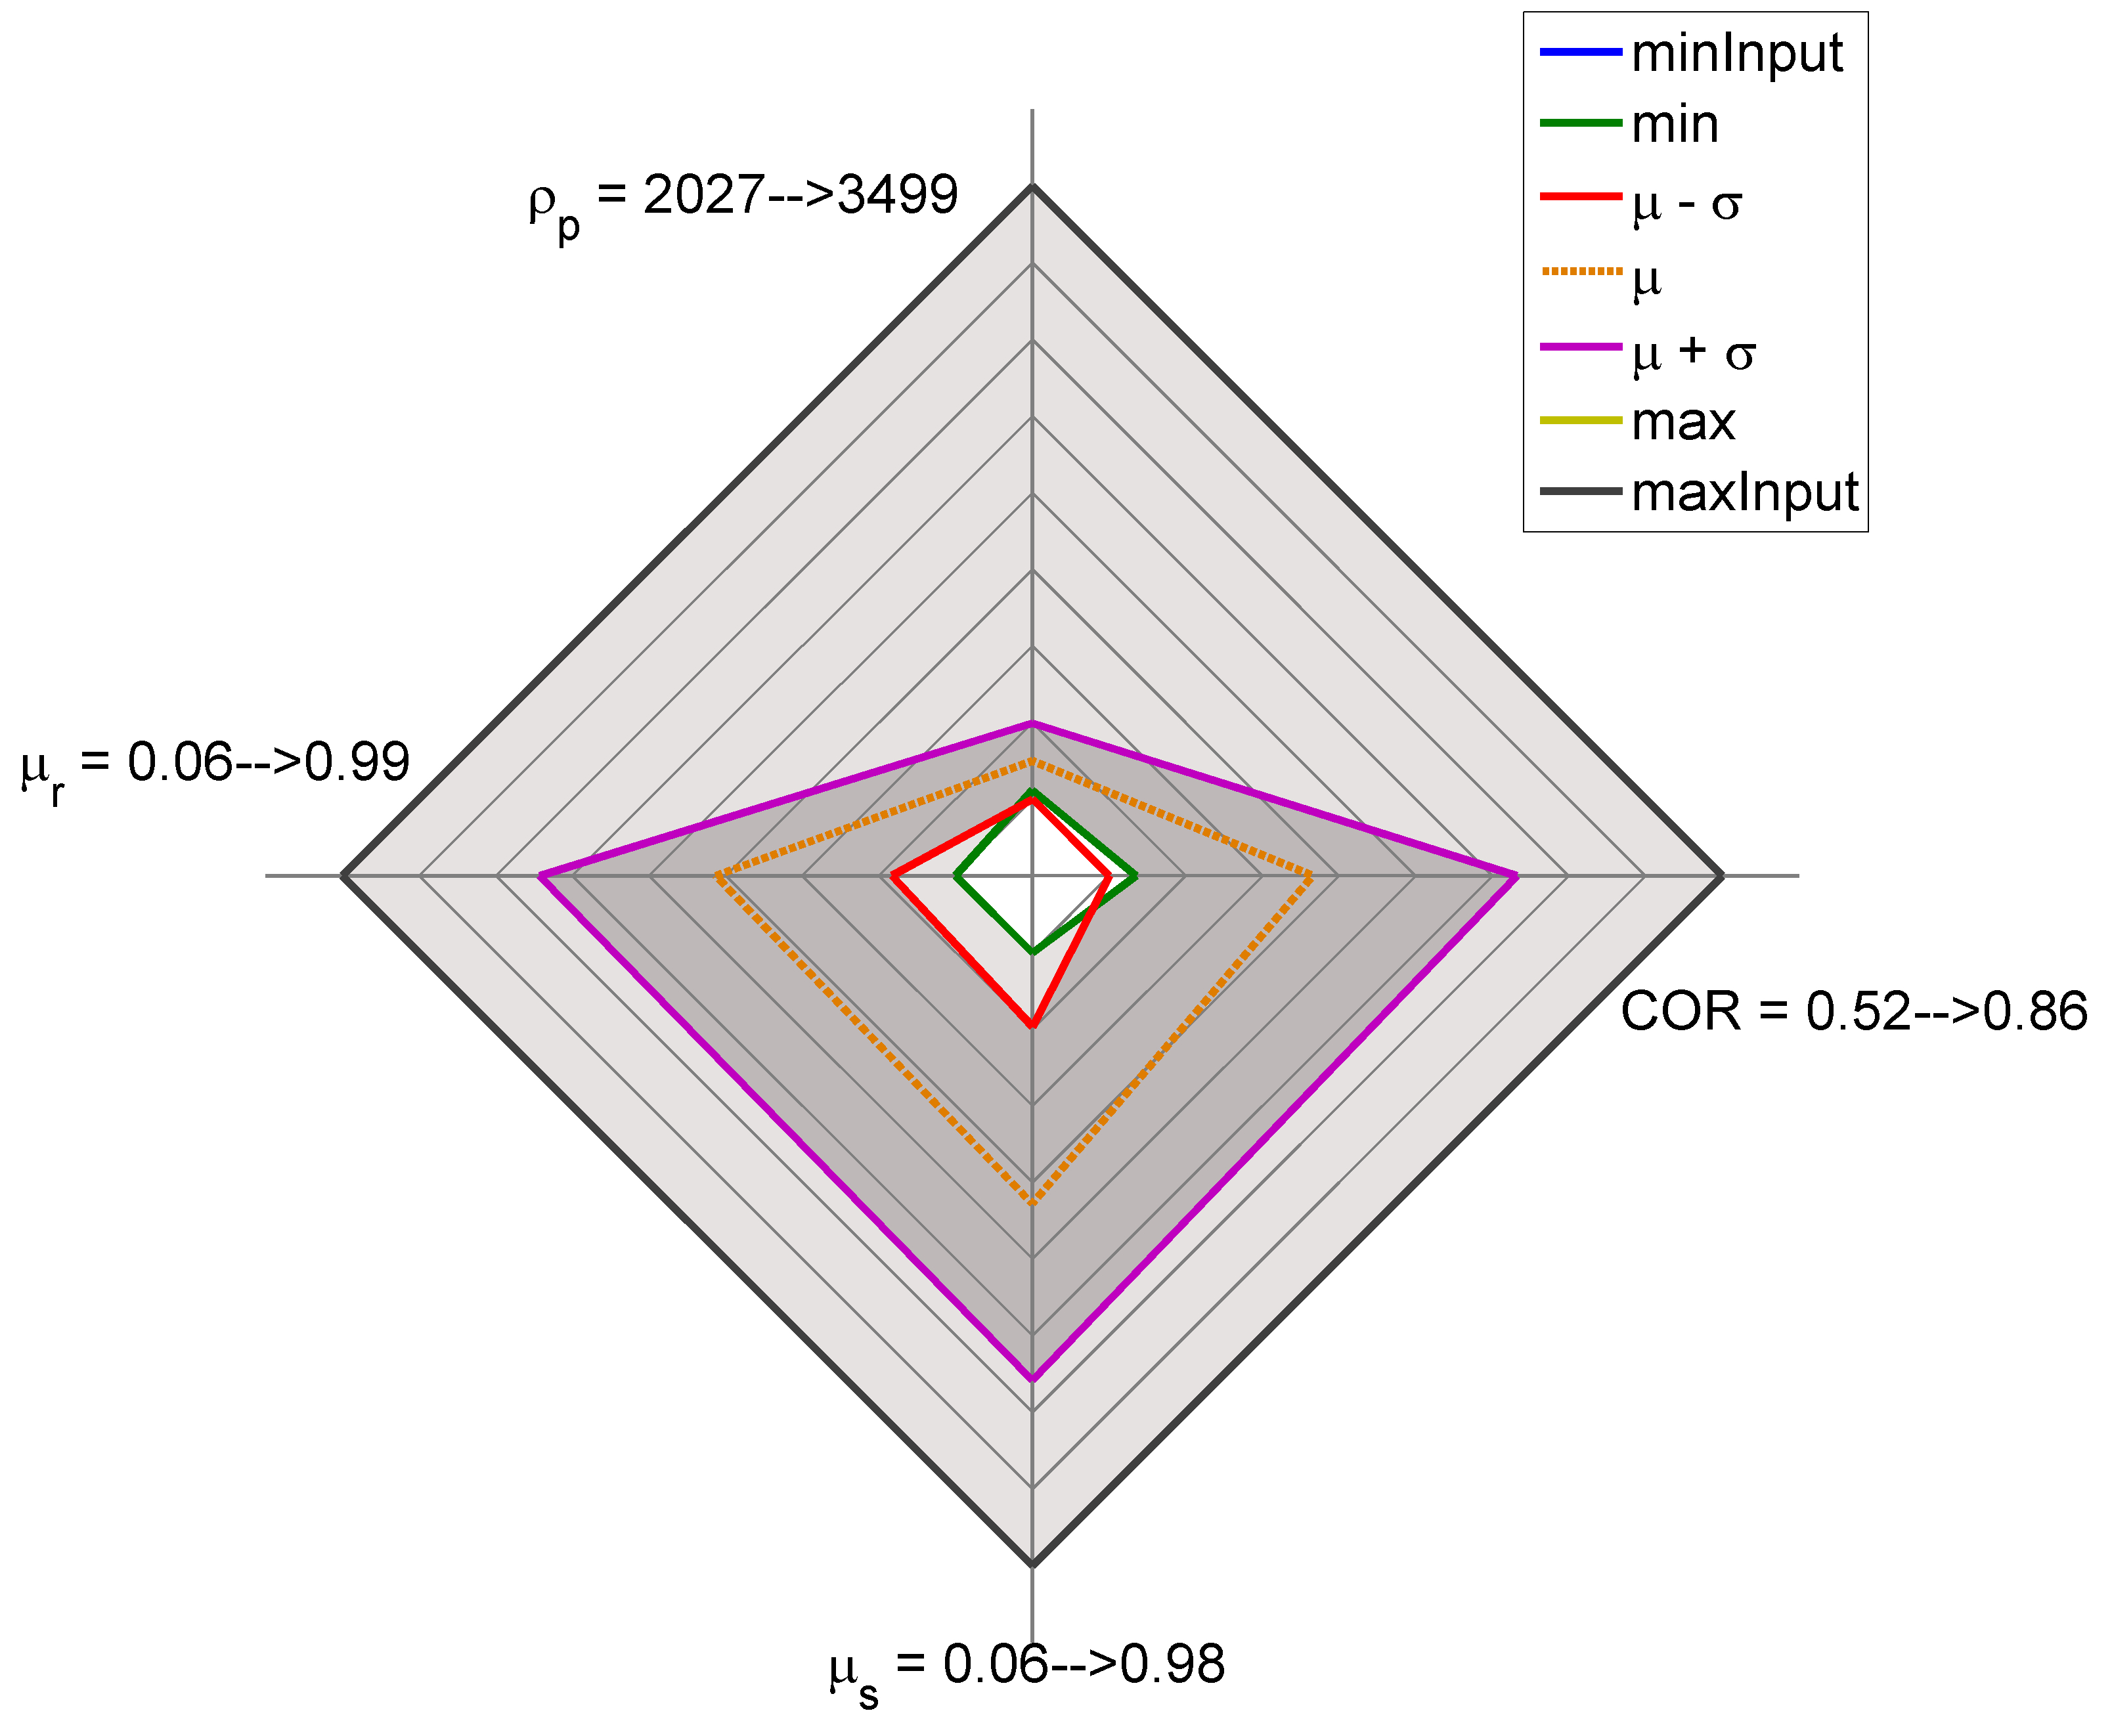
\includegraphics[width=.35\columnwidth]{images/041radarpirker1schulze1068}
	  \label{fig:041radarpirker1schulze1068}
  }
  \\
    \subfloat[Parameter space plot, \acs{SCT}, $\sigma_n=10070$ Pa, P=0.8.]{
	  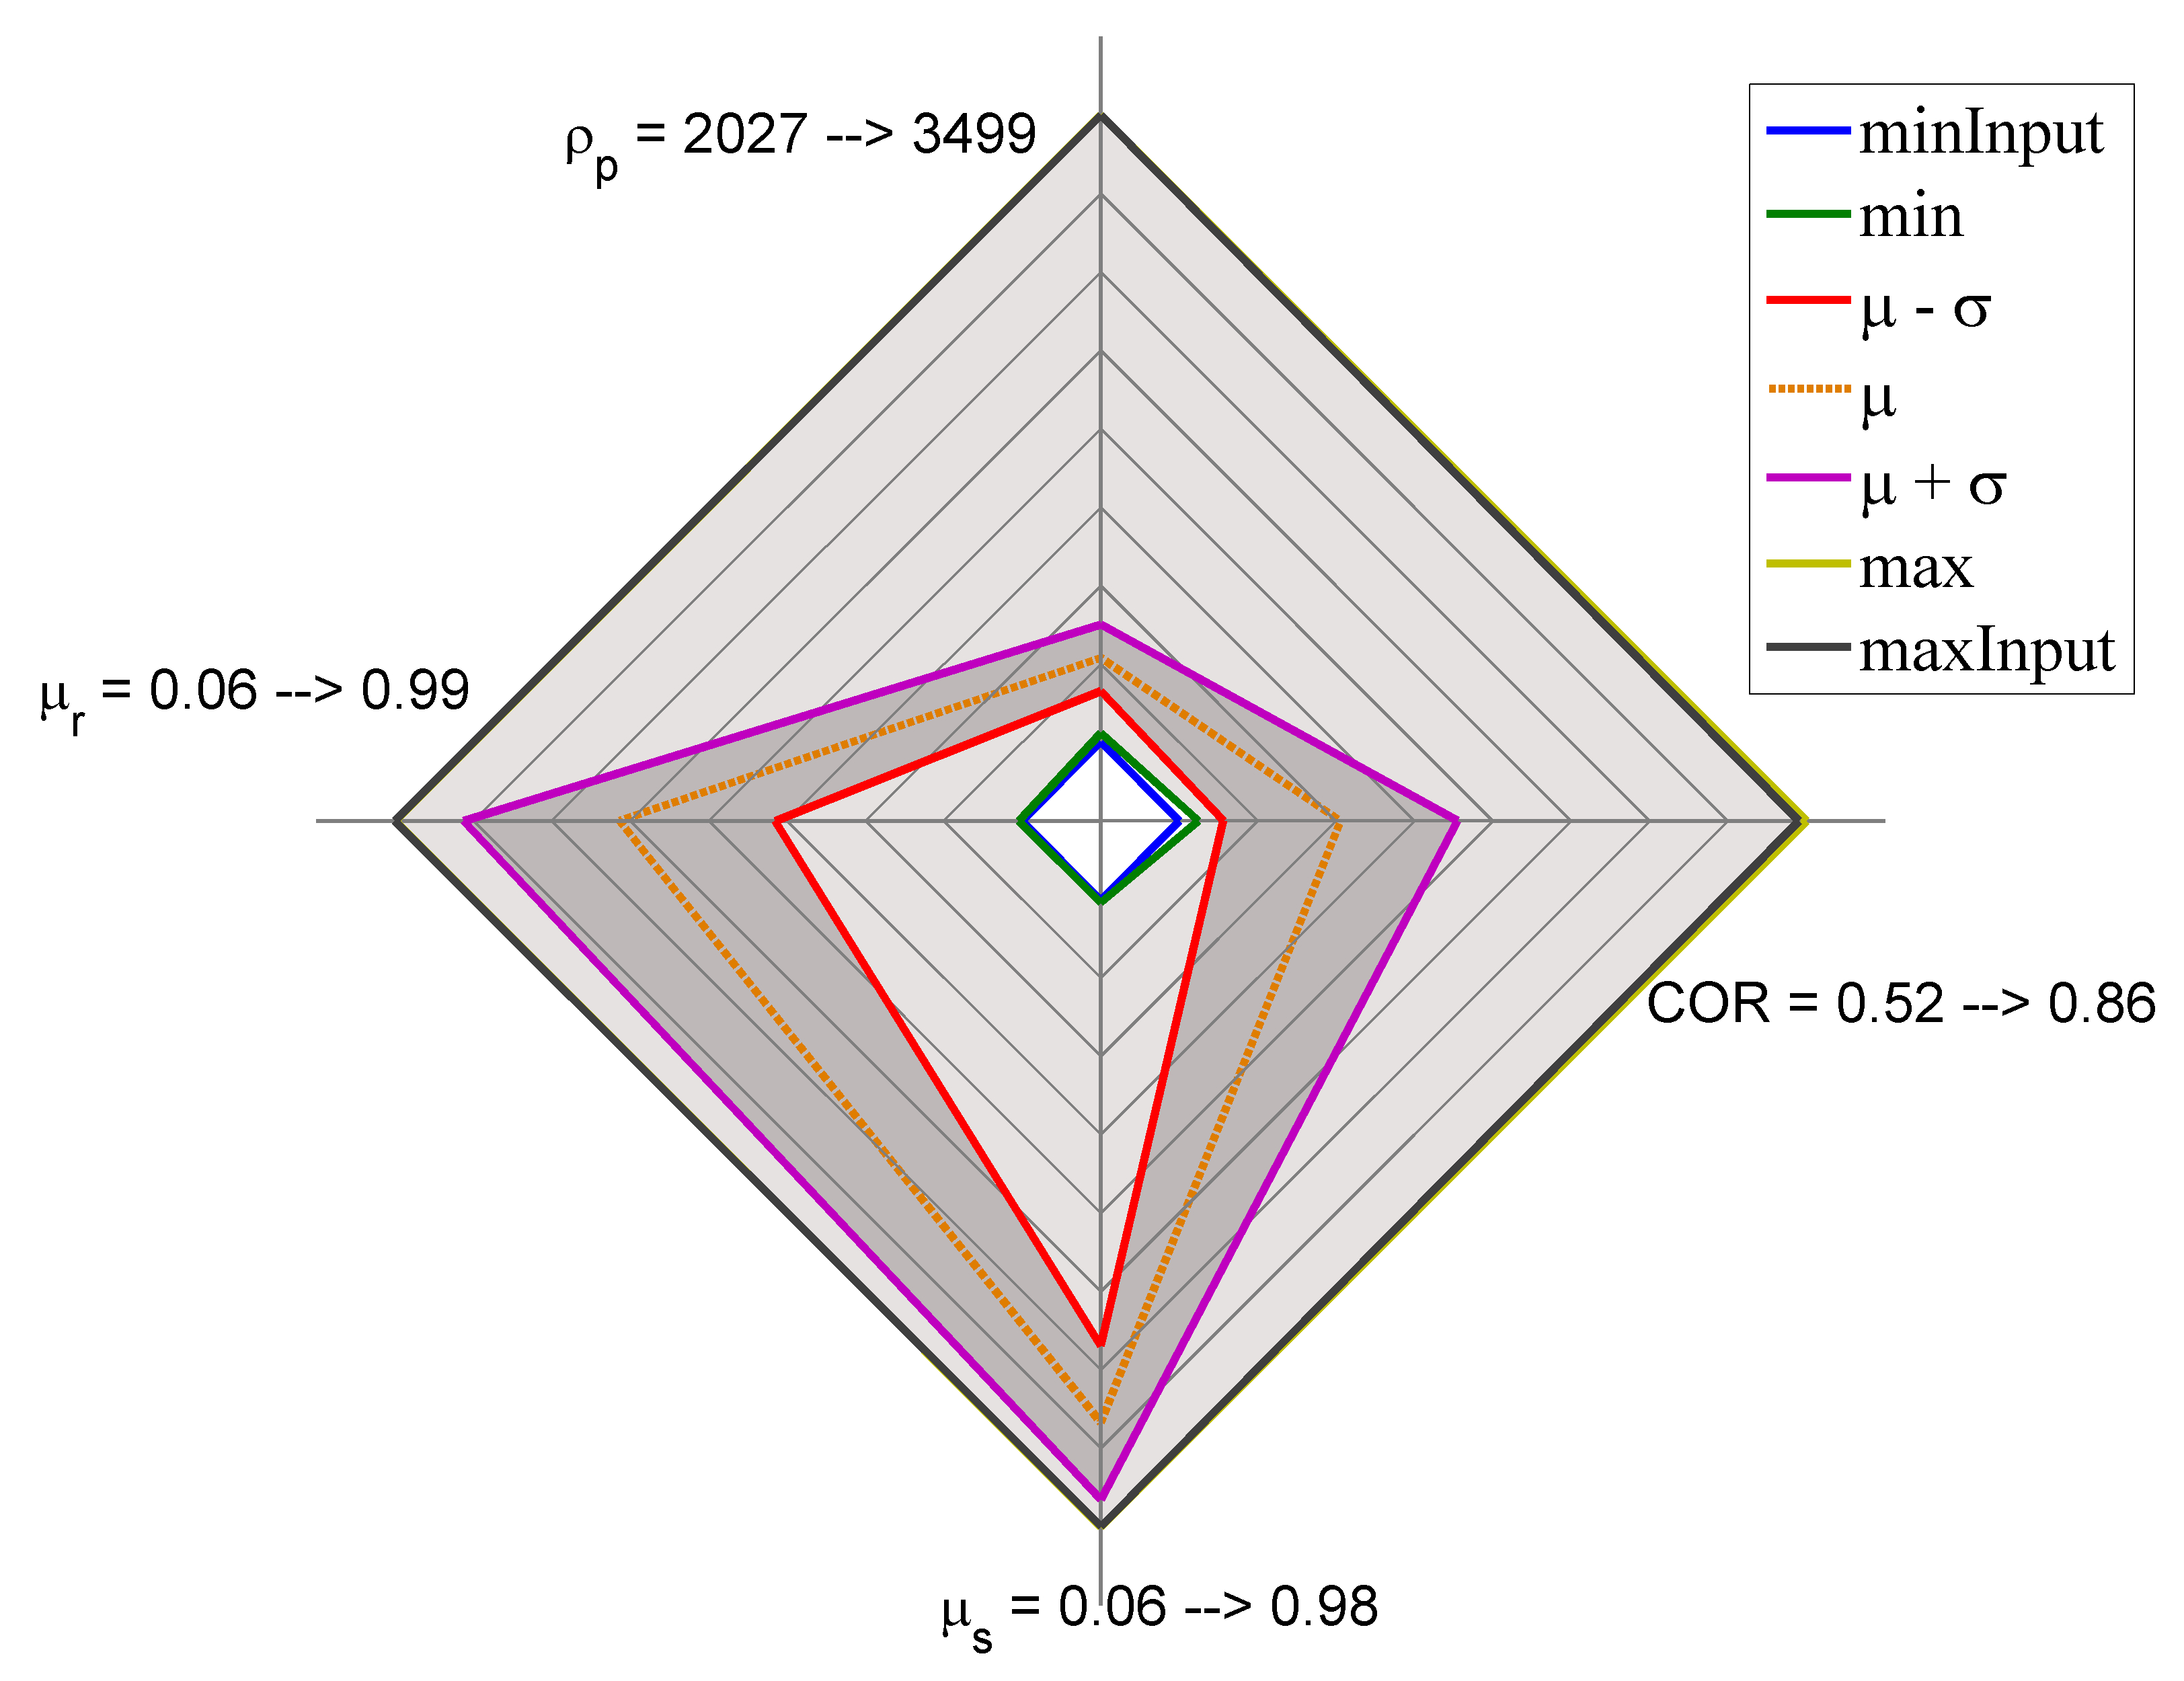
\includegraphics[width=.35\columnwidth]{images/026radarpirker08schulze10070}
	  \label{fig:026radarpirker08schulze10070}
  }
  \\
  \subfloat[Parameter space plot, \acs{SCT}, $\sigma_n=10070$ Pa, P=1.0.]{
	  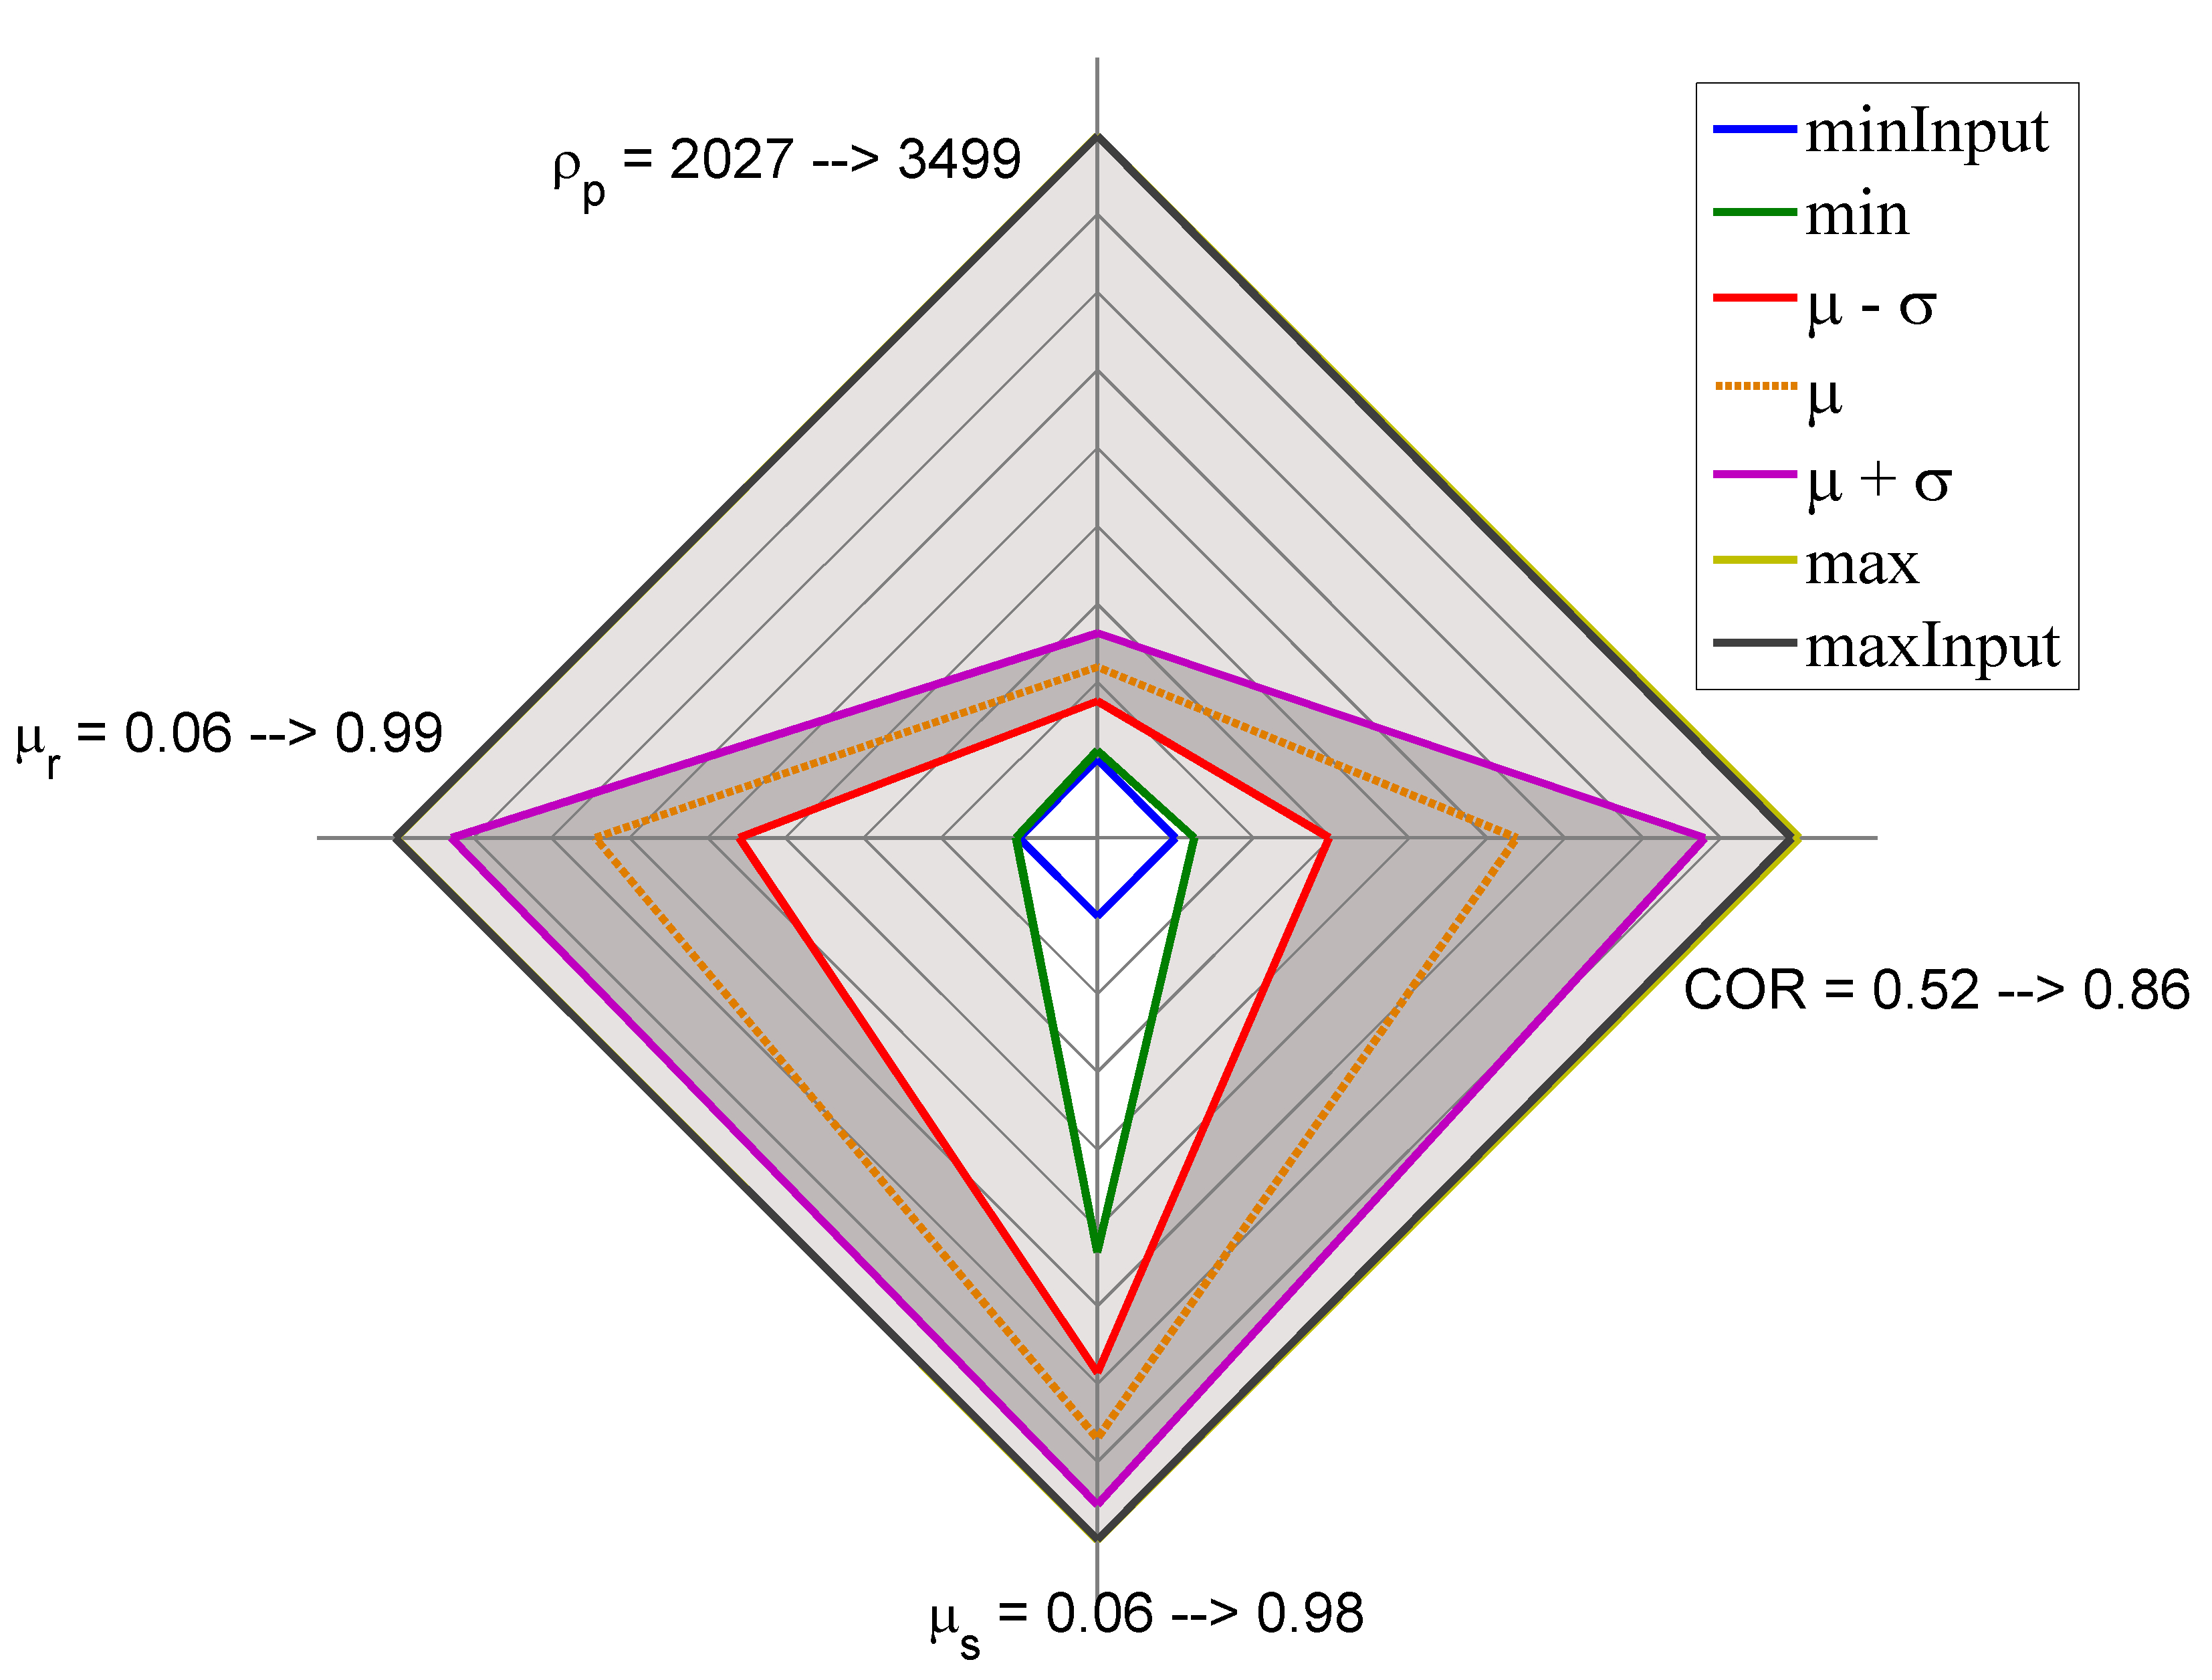
\includegraphics[width=.35\columnwidth]{images/024radarpirker1schulze10070}
	  \label{fig:024radarpirker1schulze10070}
  }
  \quad
    \subfloat[Box plot, \acs{SCT}, $\sigma_n=10070$ Pa, P=1.0.]{
	  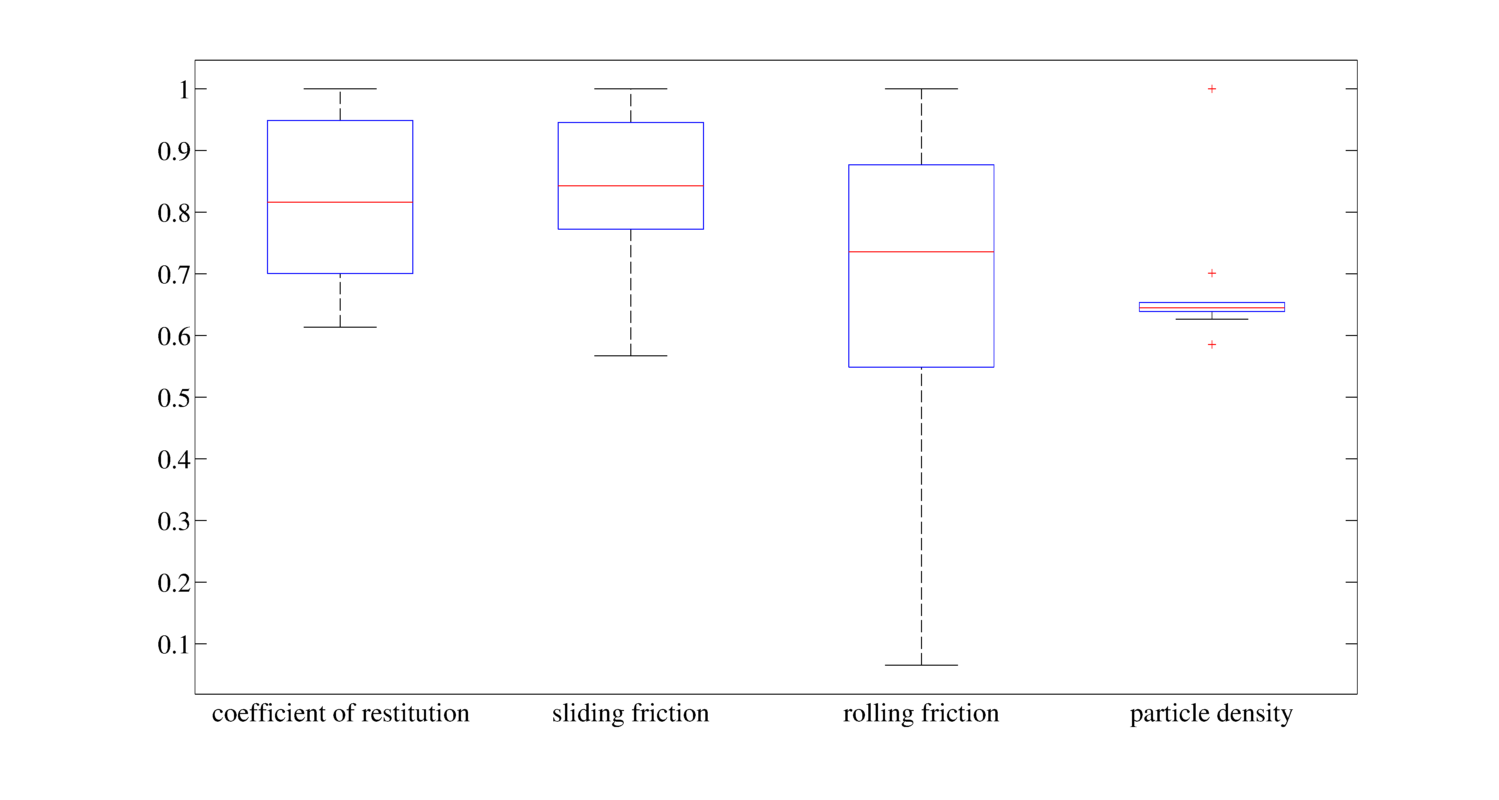
\includegraphics[width=.35\columnwidth]{images/075sctboxplot}
	  \label{fig:075sctboxplot}  }
  \\
    \subfloat[Parameter space plot, \acs{SCT}, $\sigma_n=10070$ Pa, P=1.2.]{
	  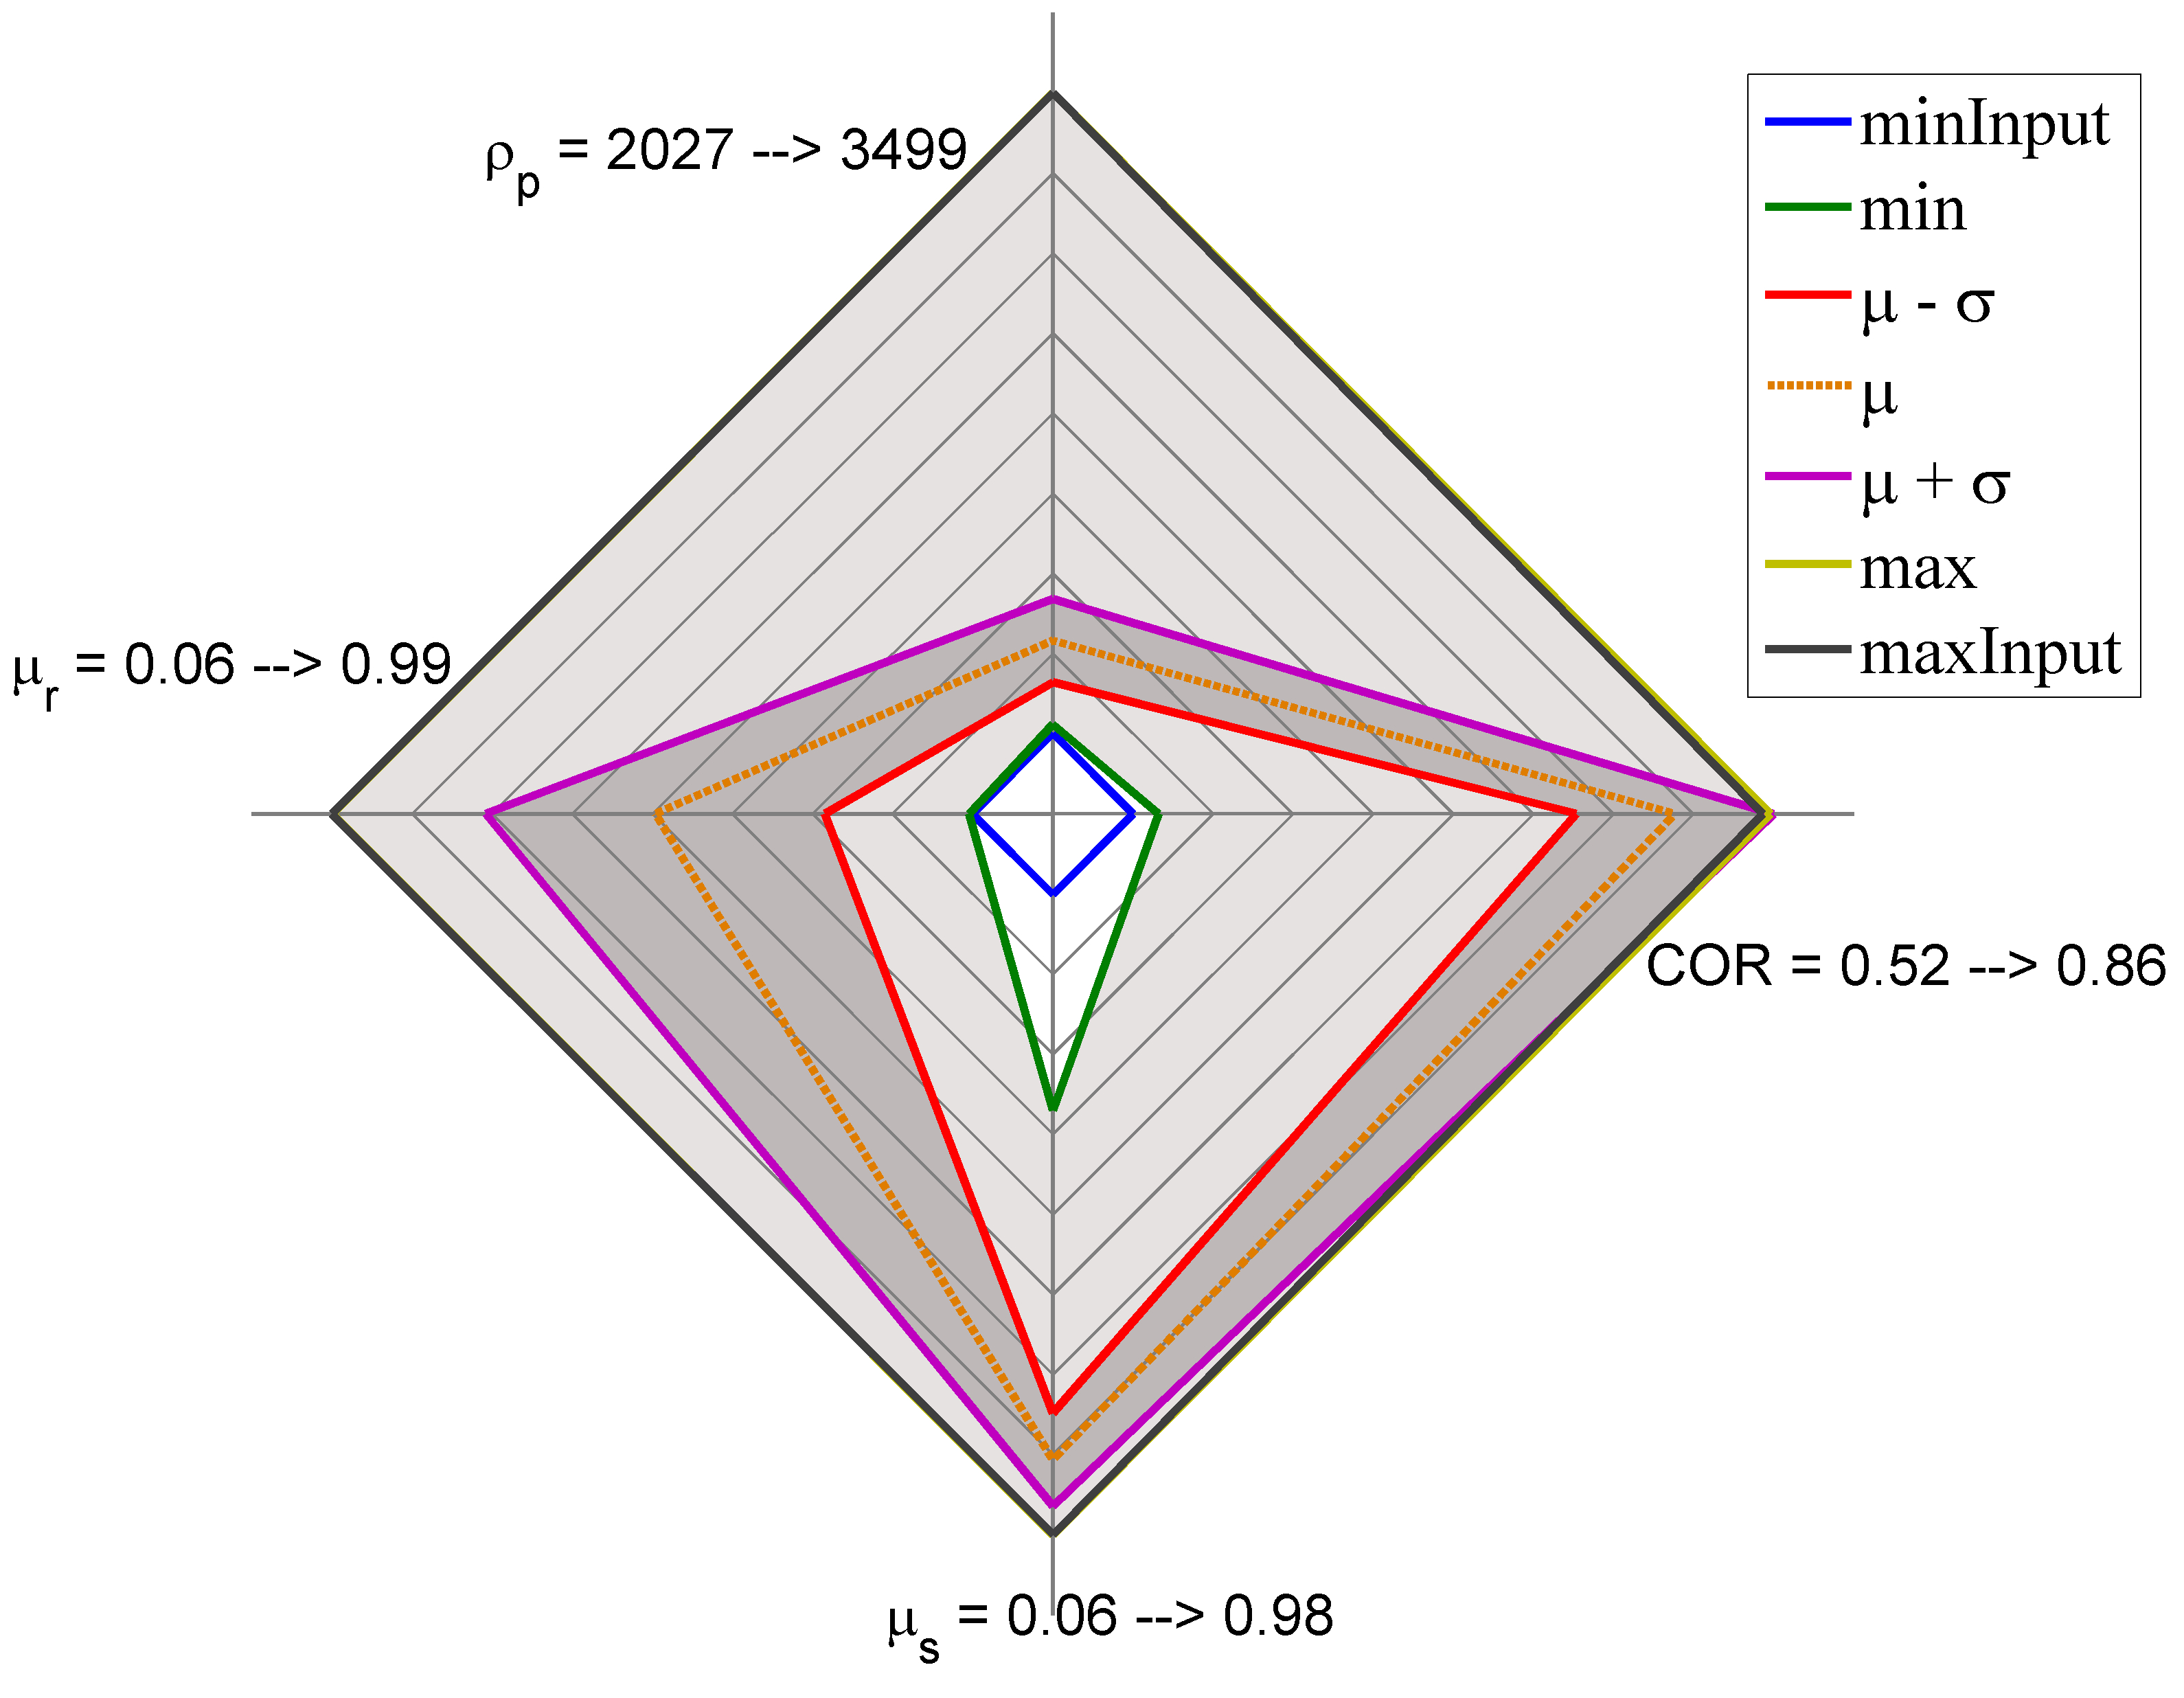
\includegraphics[width=.35\columnwidth]{images/028radarpirker12schulze10070}
	  \label{fig:028radarpirker12schulze10070}
  }
  \caption{SCT parameter space plots.}
  \label{fig:079sctparameterspaceplots}
\end{figure}

The comparison between numerical and experimental behaviours led to a first
series of marked combinations ($MC1$) for two load conditions of
the shear cell:
\begin{itemize}
  \item{$\acs{sigman} = 1,068$ Pa, P=1.0, as plotted in Fig.
  \ref{fig:041radarpirker1schulze1068},}
  \item{$\acs{sigman} = 10,070$ Pa, P=1.0, as plotted in Fig.
  \ref{fig:024radarpirker1schulze10070}.}
\end{itemize}
Note that the confidence interval is large, 
especially for the \acs{CoR}, which highlights its insignificant influence on the
characterization.
Both the \acs{rhop}  and the \acs{mus}, however, show a narrow confidence interval, 
which demonstrates their influence and the ability of this procedure to find
valid \acs{DEM} parameters.
These results agree with our examination of the ratio of the standard deviation
to the range, see Table \ref{tab:13DEMvalidvalues}.

\subsection{SCT box plot for Sinter fine}
\label{subsec:sctboxsinterfine}

The representation through box plots in Fig.
\ref{fig:156boxplotsct10070sinterfine} is consistent with those shown in the
previous Section \ref{subsec:sctparameterspacesinterfine}.

\begin{figure}[htbp]
\centering 
%   \subfloat[Parameter space plot, \acs{SCT}, $\sigma_n=1068$ Pa, P=1.0.]{
% 	  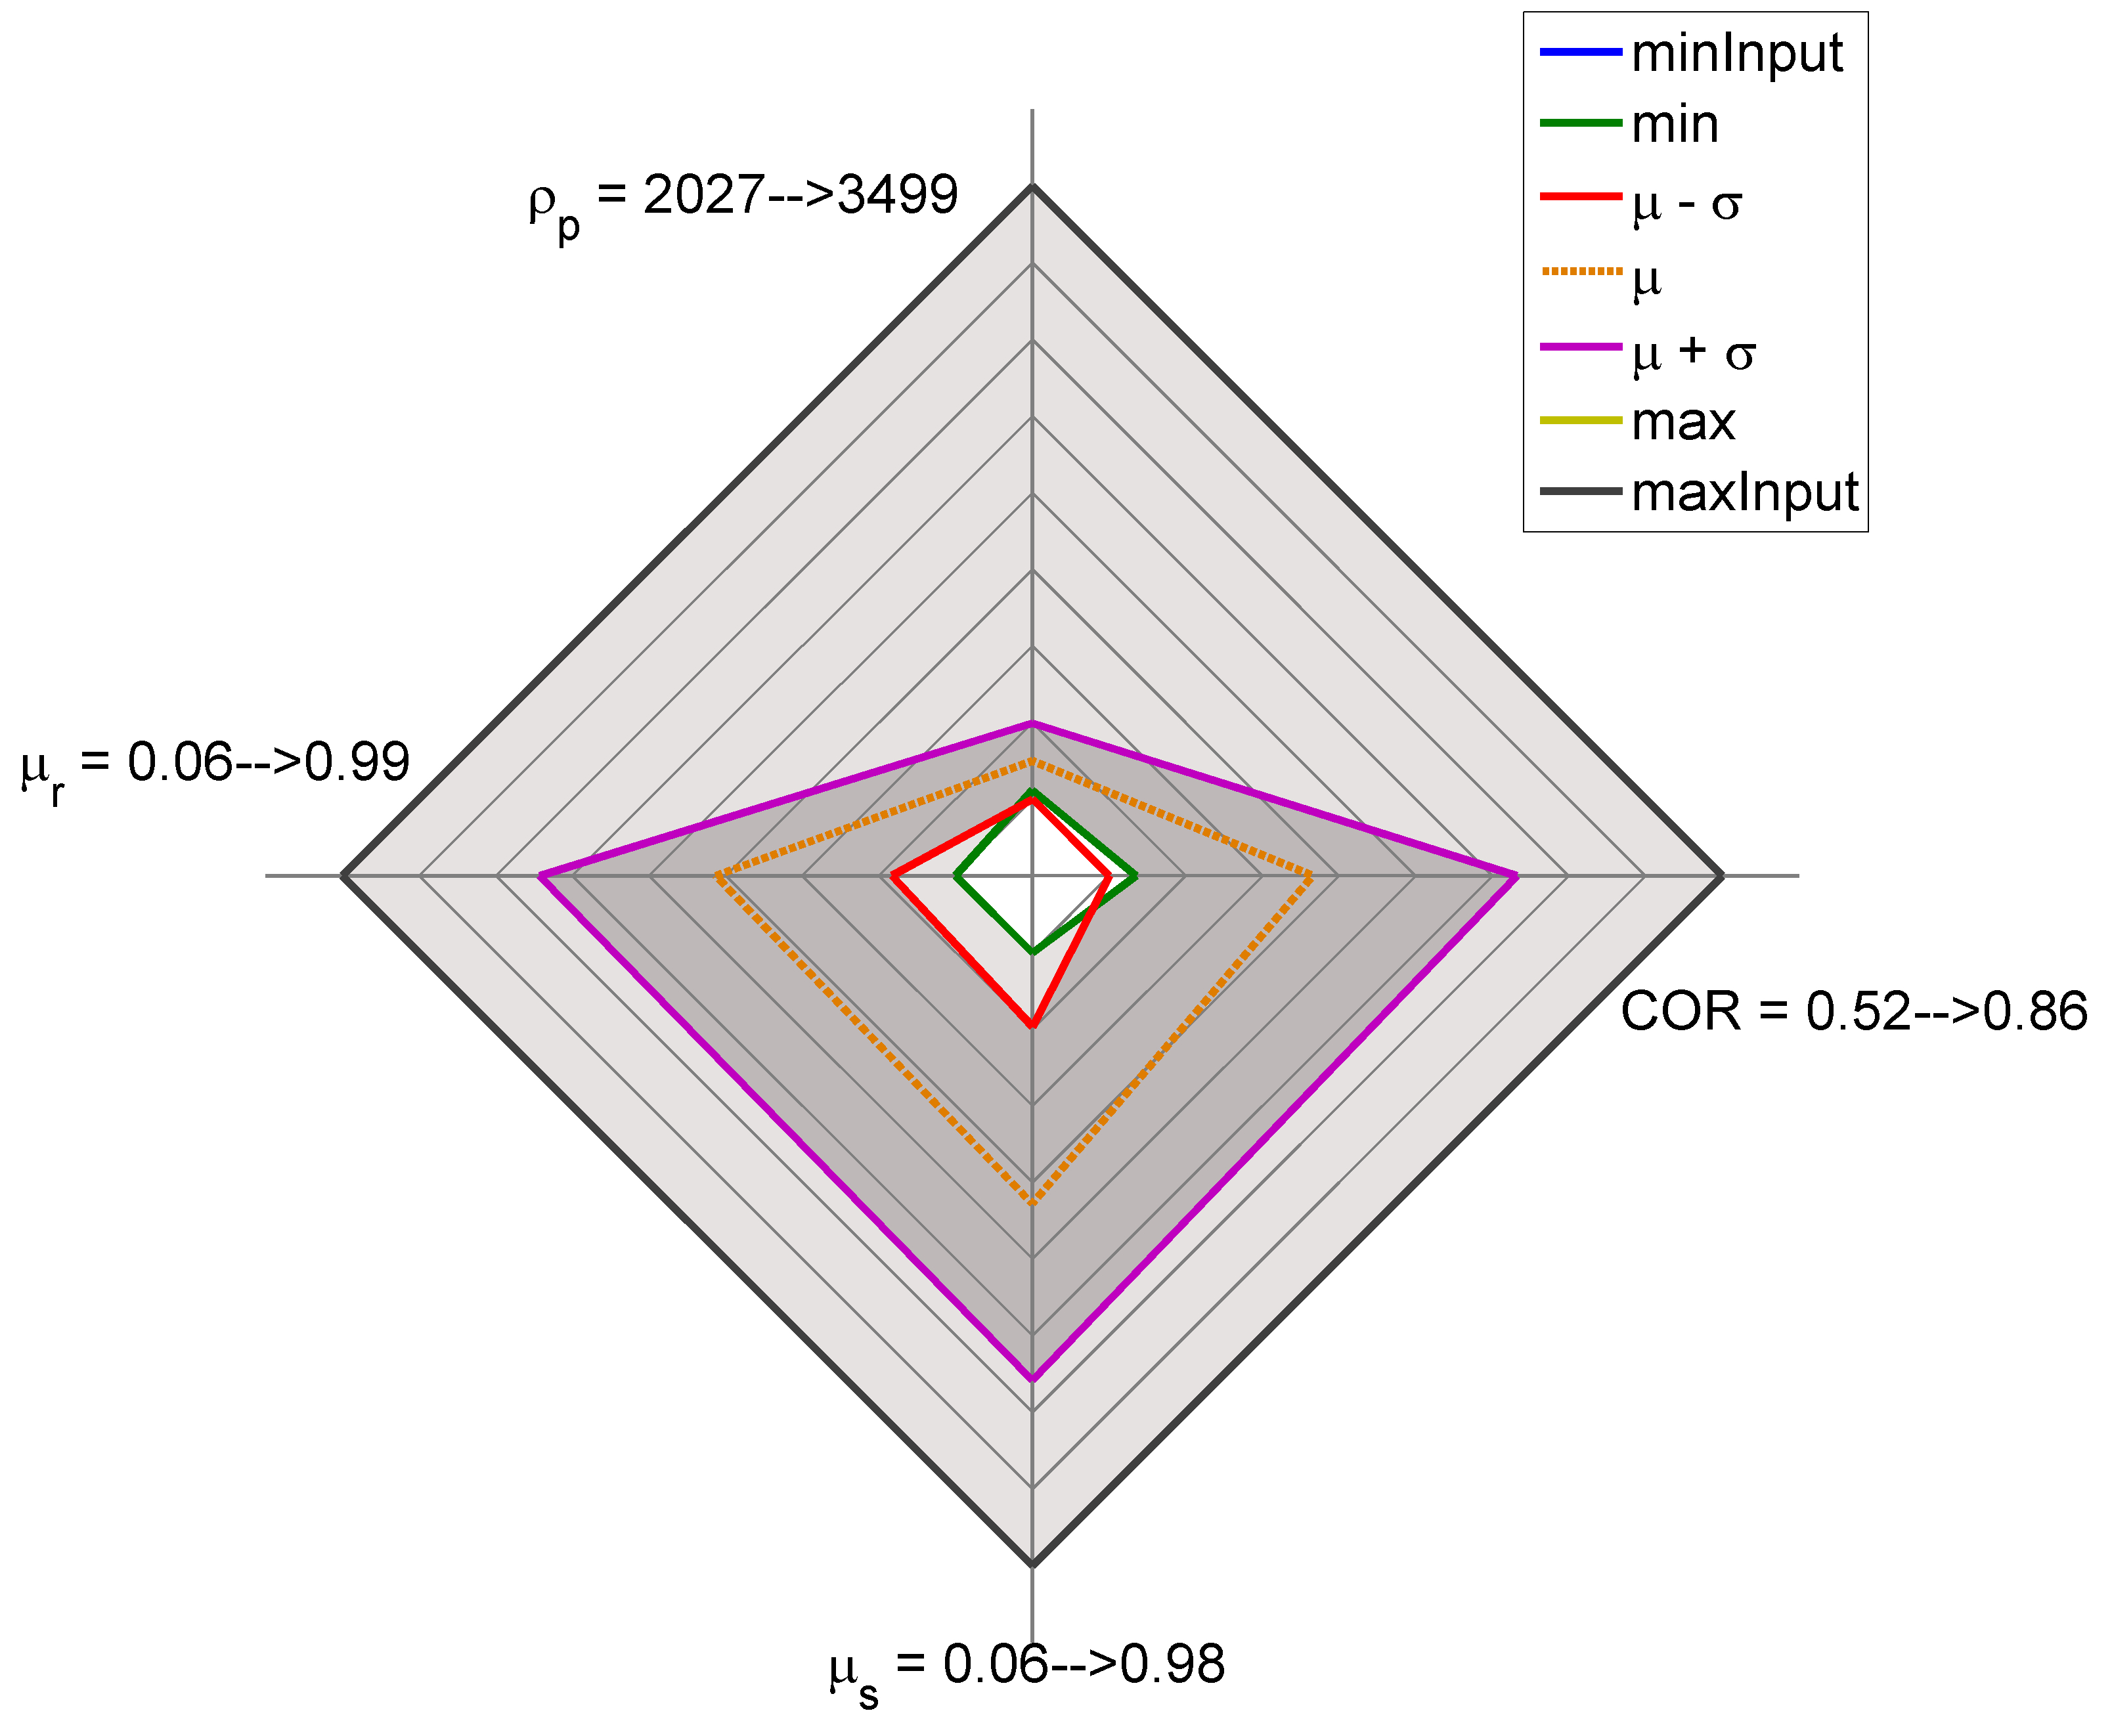
\includegraphics[width=.35\columnwidth]{images/041radarpirker1schulze1068}
% 	  \label{fig:041radarpirker1schulze1068}
%   }
%   \\157BoxSCT10070p08sinterfine.png
%158BoxSCT10070p12sinterfine.png
    \subfloat[Box plot, \acs{SCT}, $\sigma_n=10070$ Pa, P=0.8.]{
	  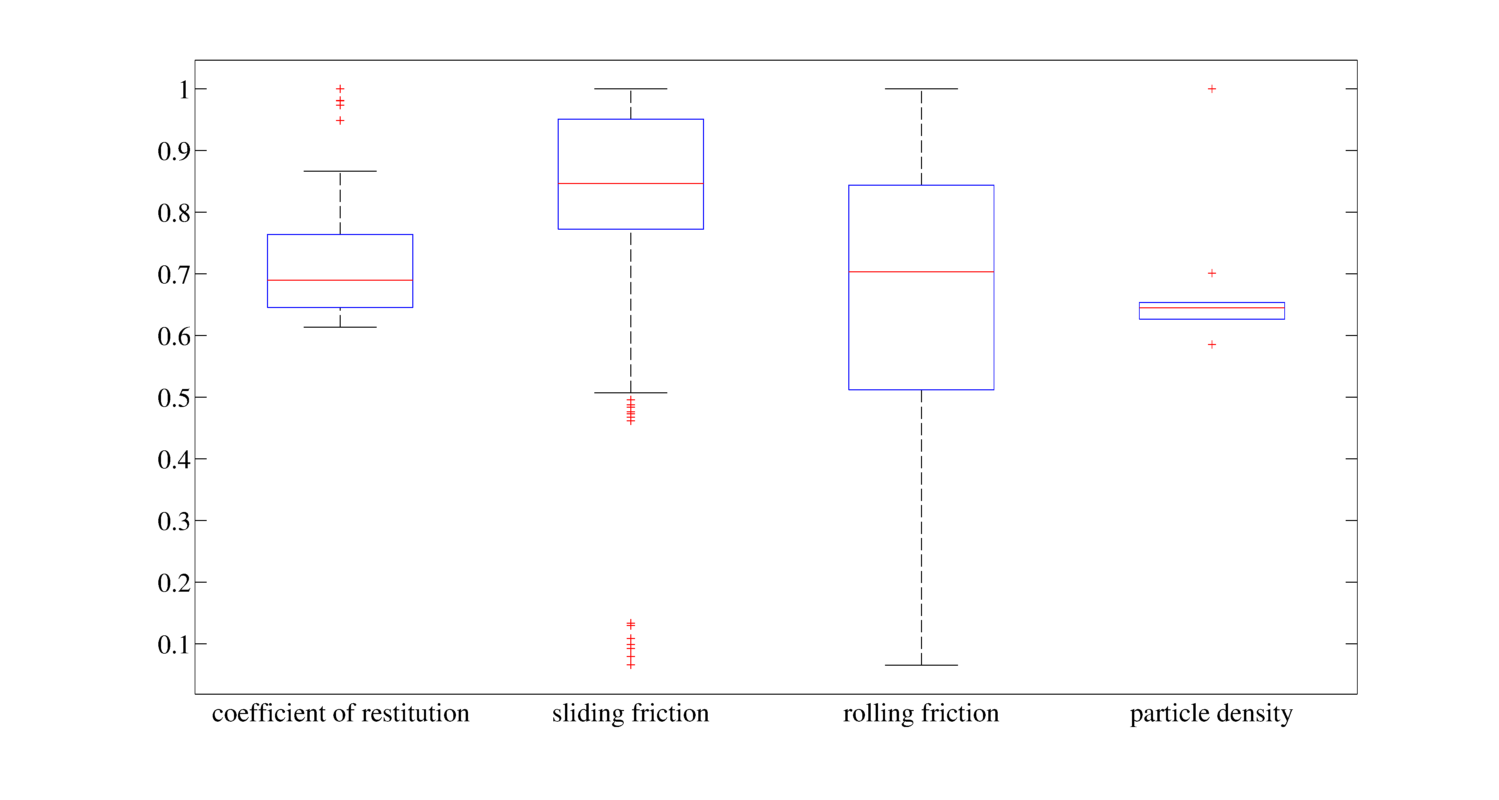
\includegraphics[width=.70\columnwidth]{images/157BoxSCT10070p08sinterfine}
	  \label{fig:157BoxSCT10070p08sinterfine}  }
  \\
    \subfloat[Box plot, \acs{SCT}, $\sigma_n=10070$ Pa, P=1.0.]{
	  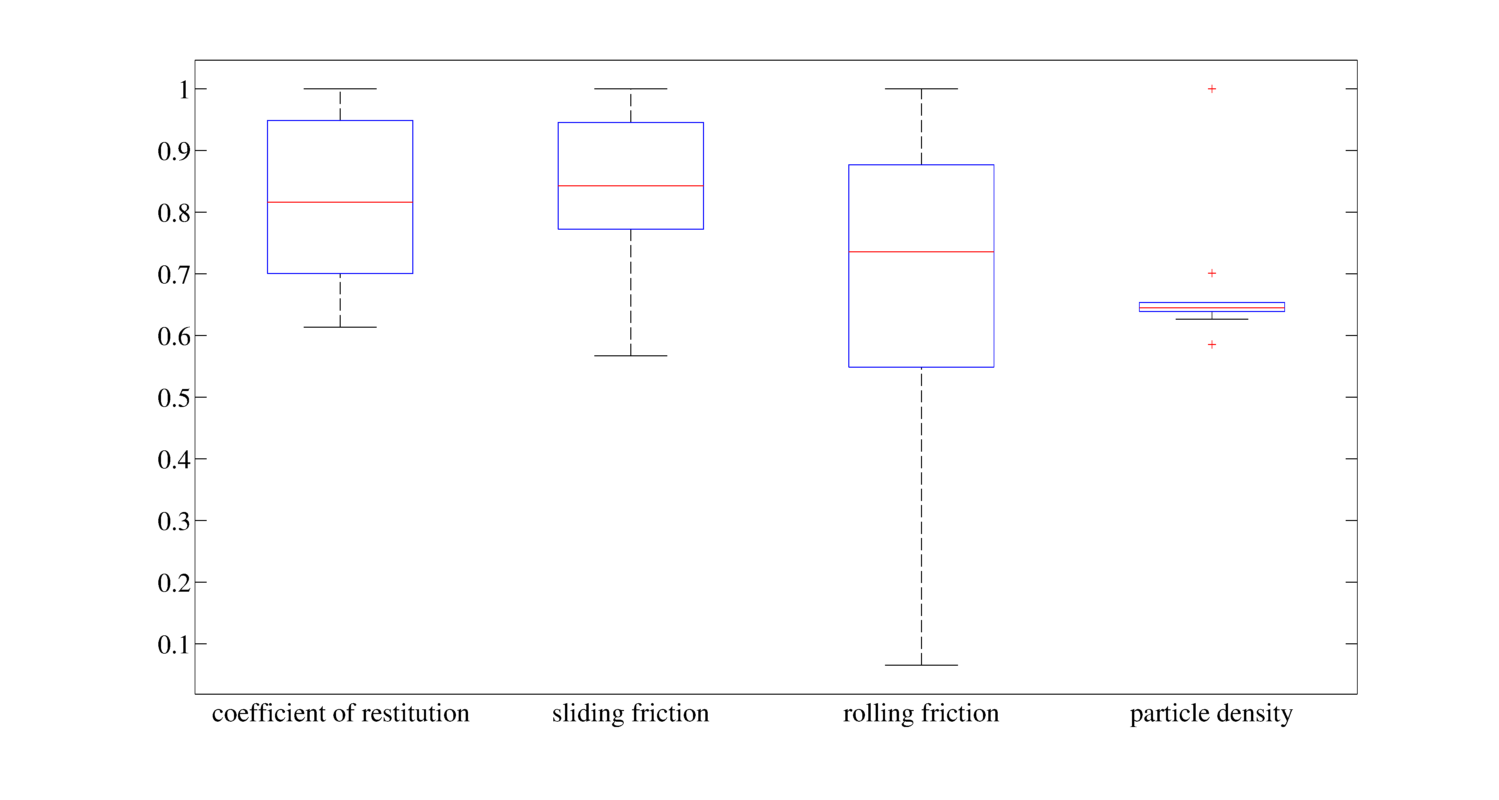
\includegraphics[width=.70\columnwidth]{images/075sctboxplot}
	  \label{fig:075sctboxplot}  }
  \\
    \subfloat[Box plot, \acs{SCT}, $\sigma_n=10070$ Pa, P=1.2.]{
	  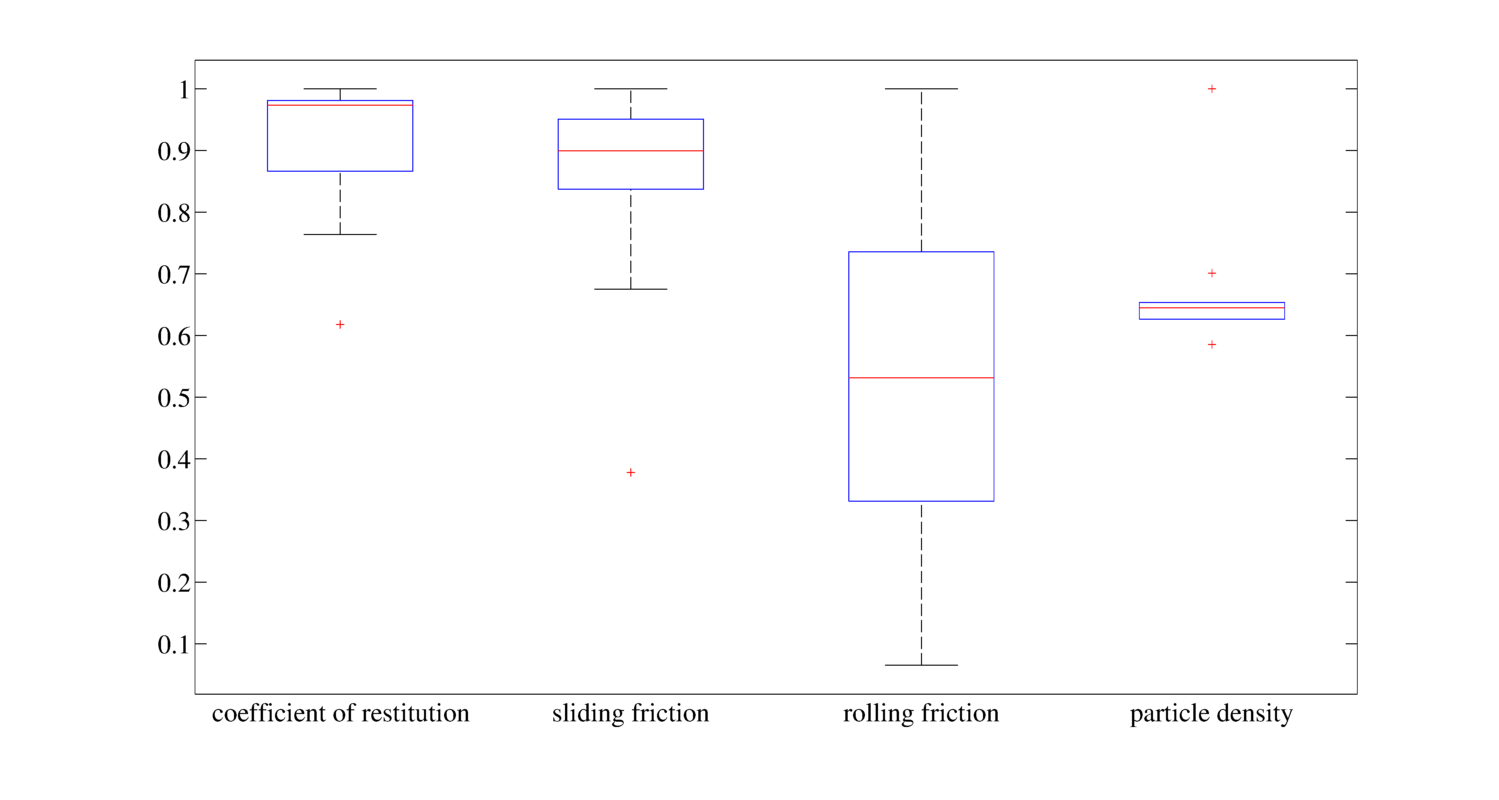
\includegraphics[width=.70\columnwidth]{images/158BoxSCT10070p12sinterfine}
	  \label{fig:158BoxSCT10070p12sinterfine}  }
  \\
  \caption[SCT box plots for sinter fine]{SCT box
  plots for sinter fine, $\sigma_n=10070$ Pa. The range of valid parameters is
  shown, together with the average and the 25 and 75 percentile.}
  \label{fig:156boxplotsct10070sinterfine}
\end{figure}

\subsection{SCT cloud space}
\label{subsec:sctcloudspace}

Multiple
combinations (250,407 or 4\% of the total) of \acs{mus} and \acs{mur} reproduced
the experimental behaviour with varying \acs{CoR}.
This underlines once more their correlation, as already stated by Wensrich and 
Katterfeld \cite{RefWorks:87}.

\begin{figure}[htbp]
\centering 
  \subfloat[Density plot, $SSC$, $\sigma_n=10070$ Pa, P=0.8.]{
	  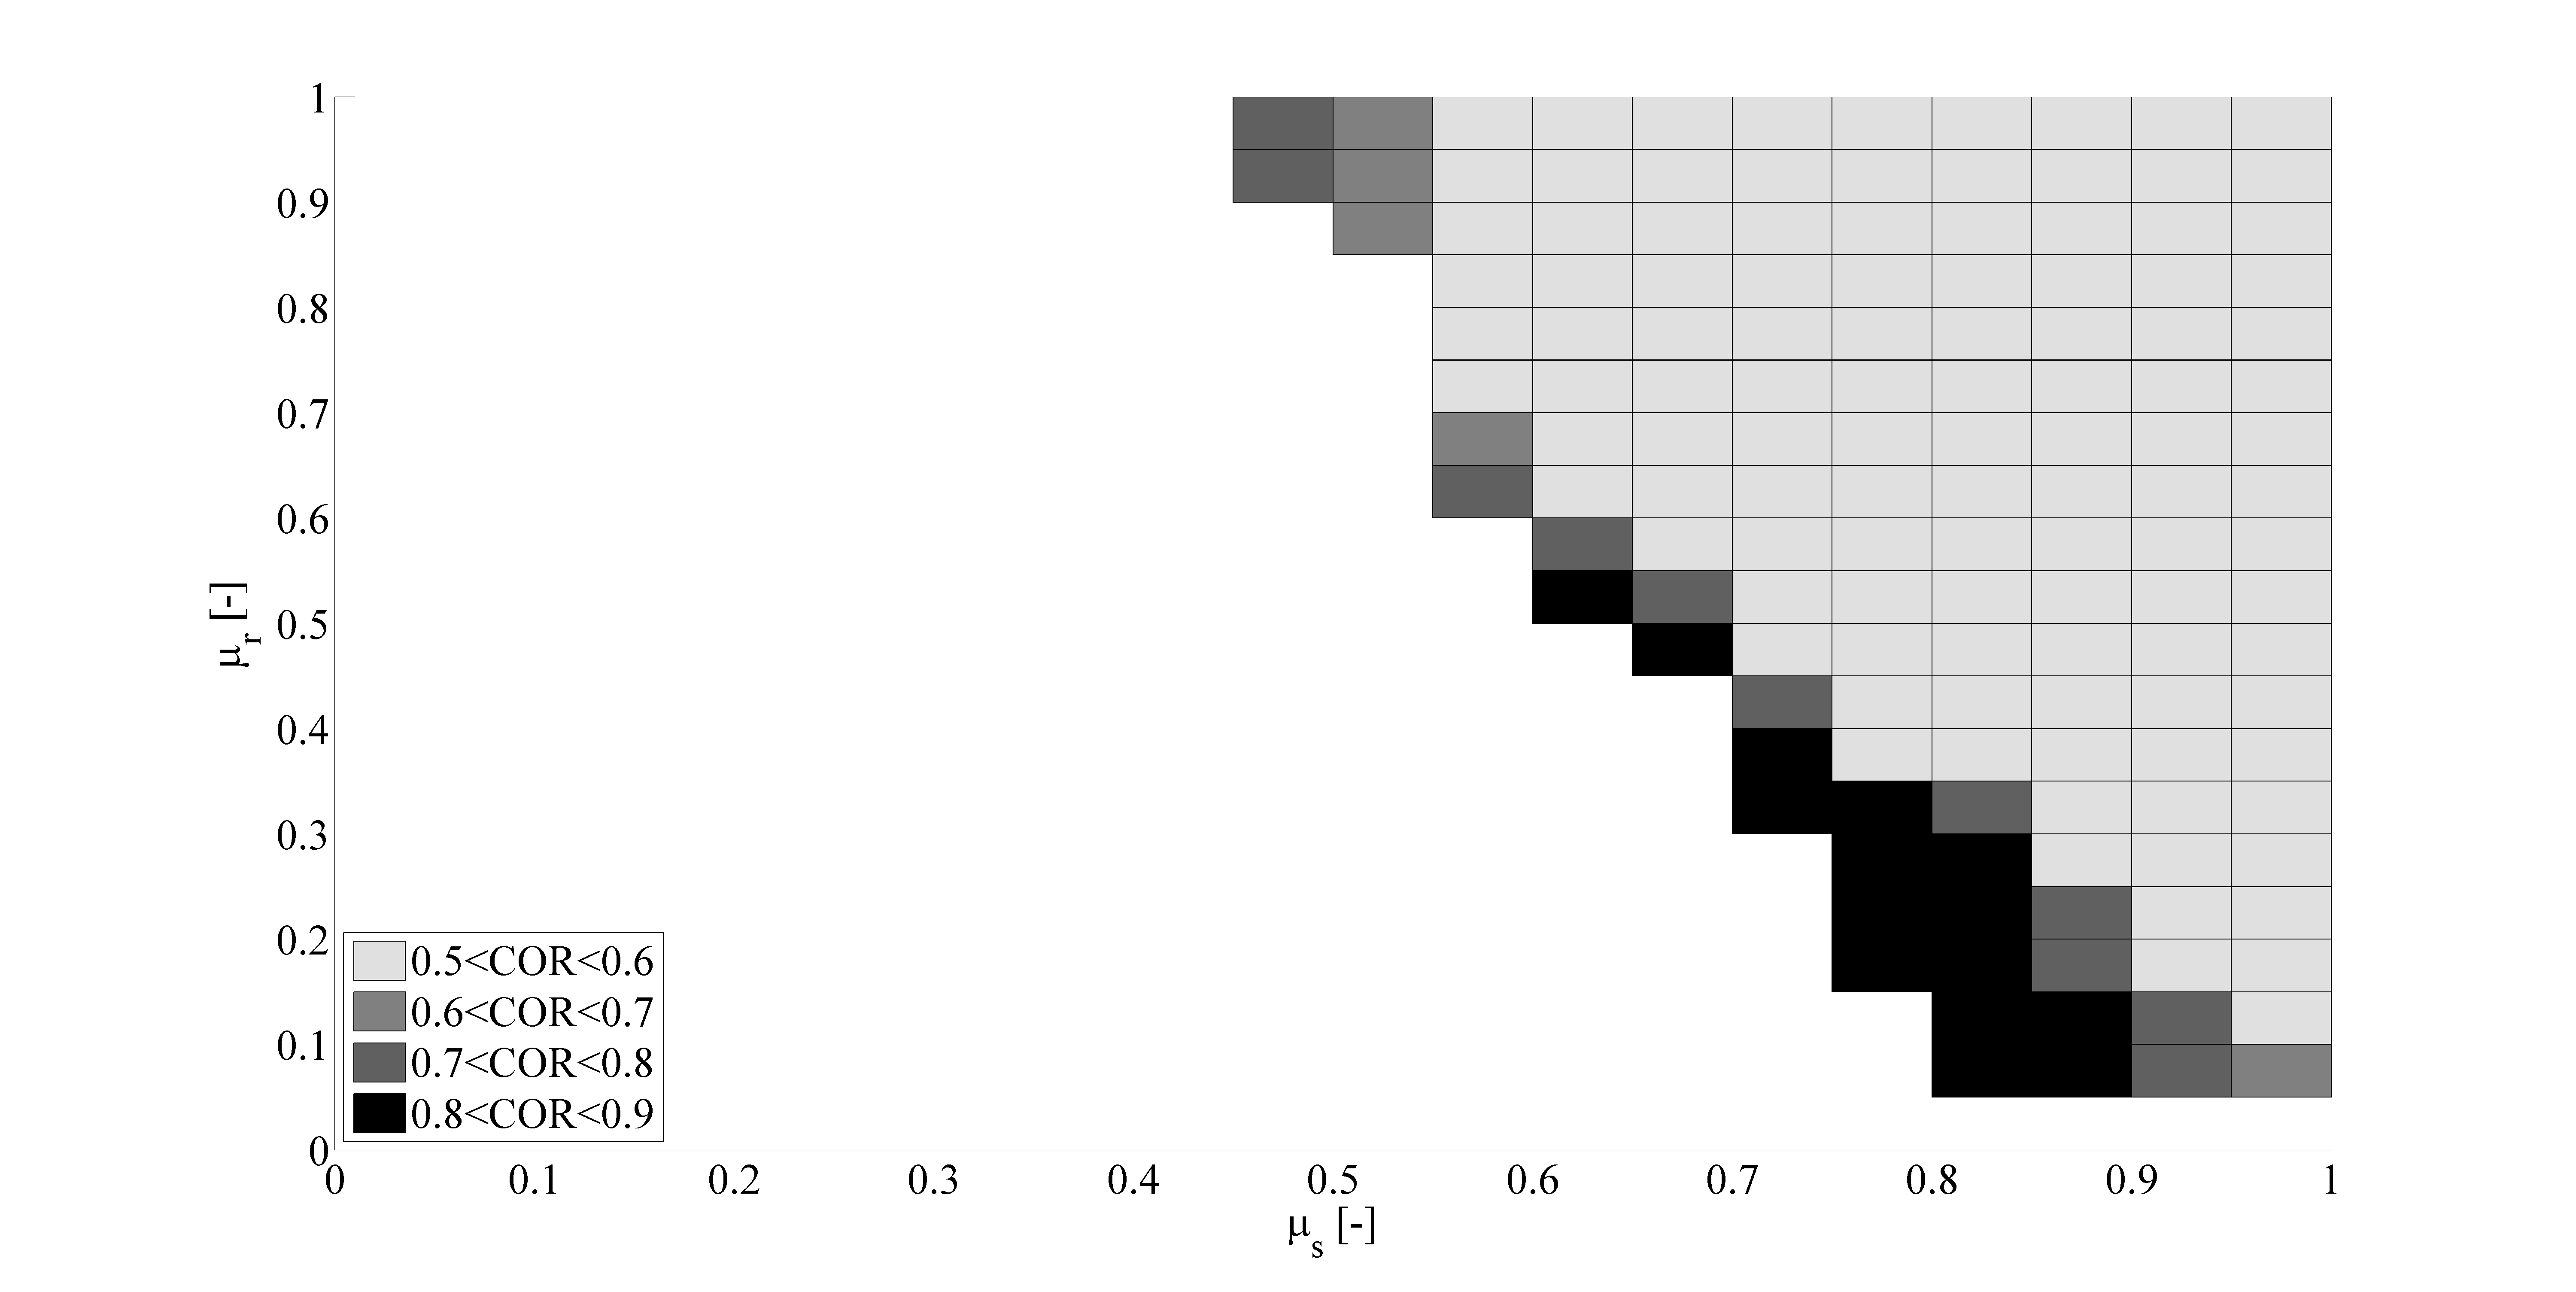
\includegraphics[width=.48\columnwidth]{images/027cloudpirker08schulze10070}
	  \label{fig:027cloudpirker08schulze10070}
  }
  \\
    \subfloat[Density plot, $SSC$, $\sigma_n=10070$ Pa, P=1.0.]{
	  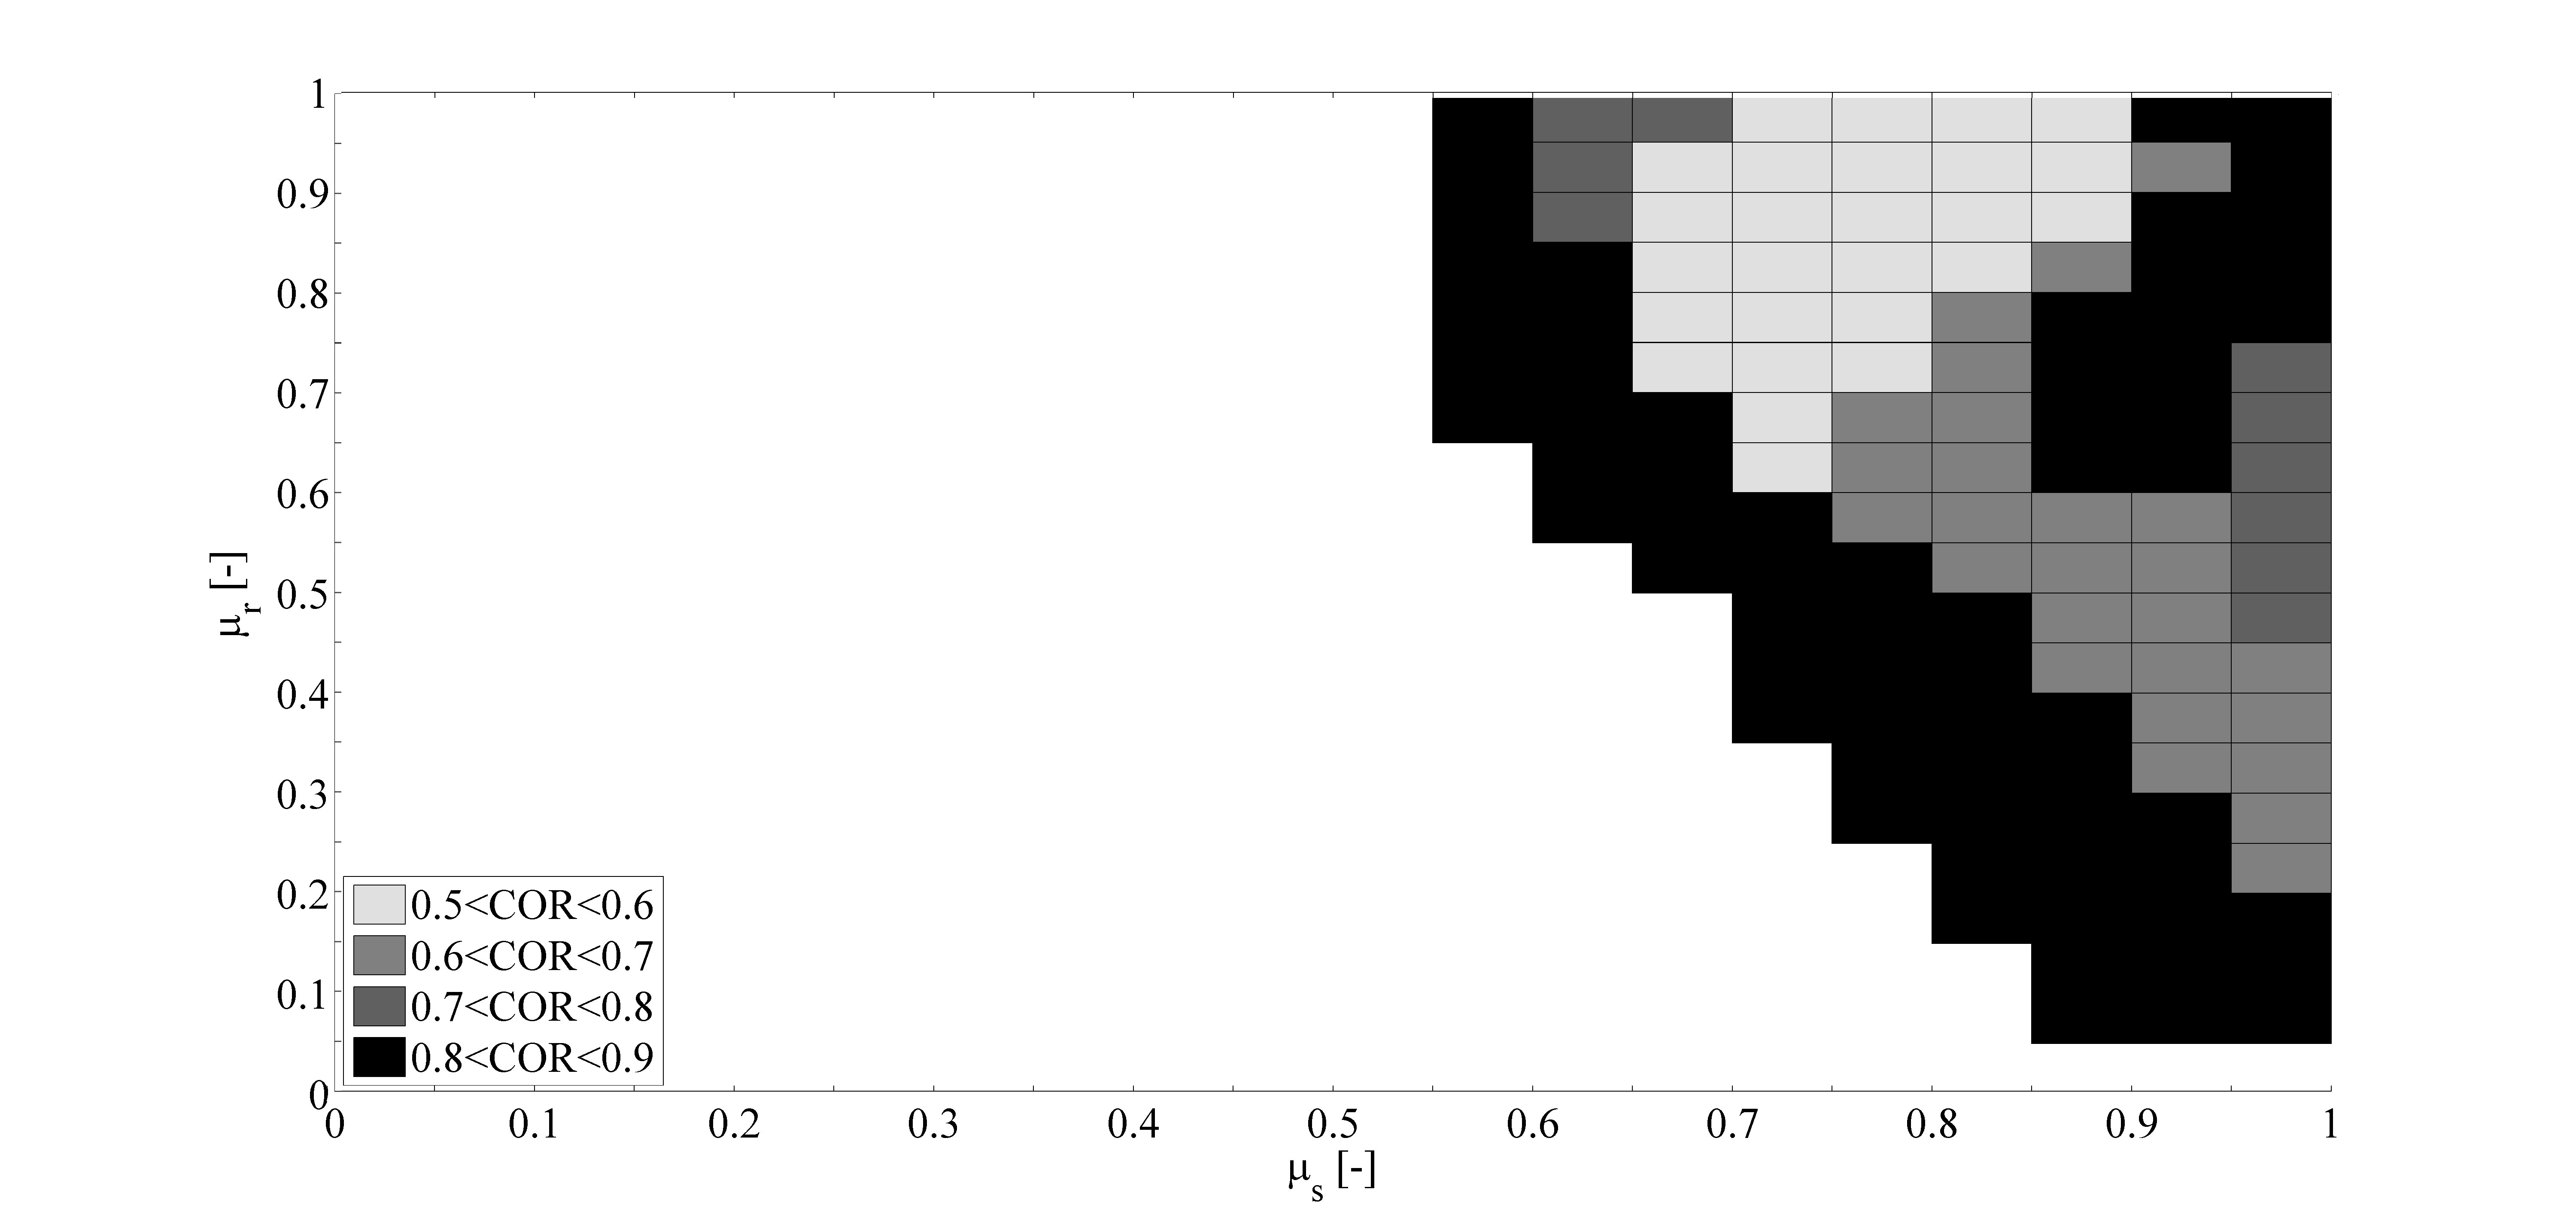
\includegraphics[width=.48\columnwidth]{images/025cloudpirker1schulze10070}
	  \label{fig:025cloudpirker1schulze10070}
  }
  \\
  \subfloat[Density plot, $SSC$, $\sigma_n=10070$ Pa, P=1.2.]{
	  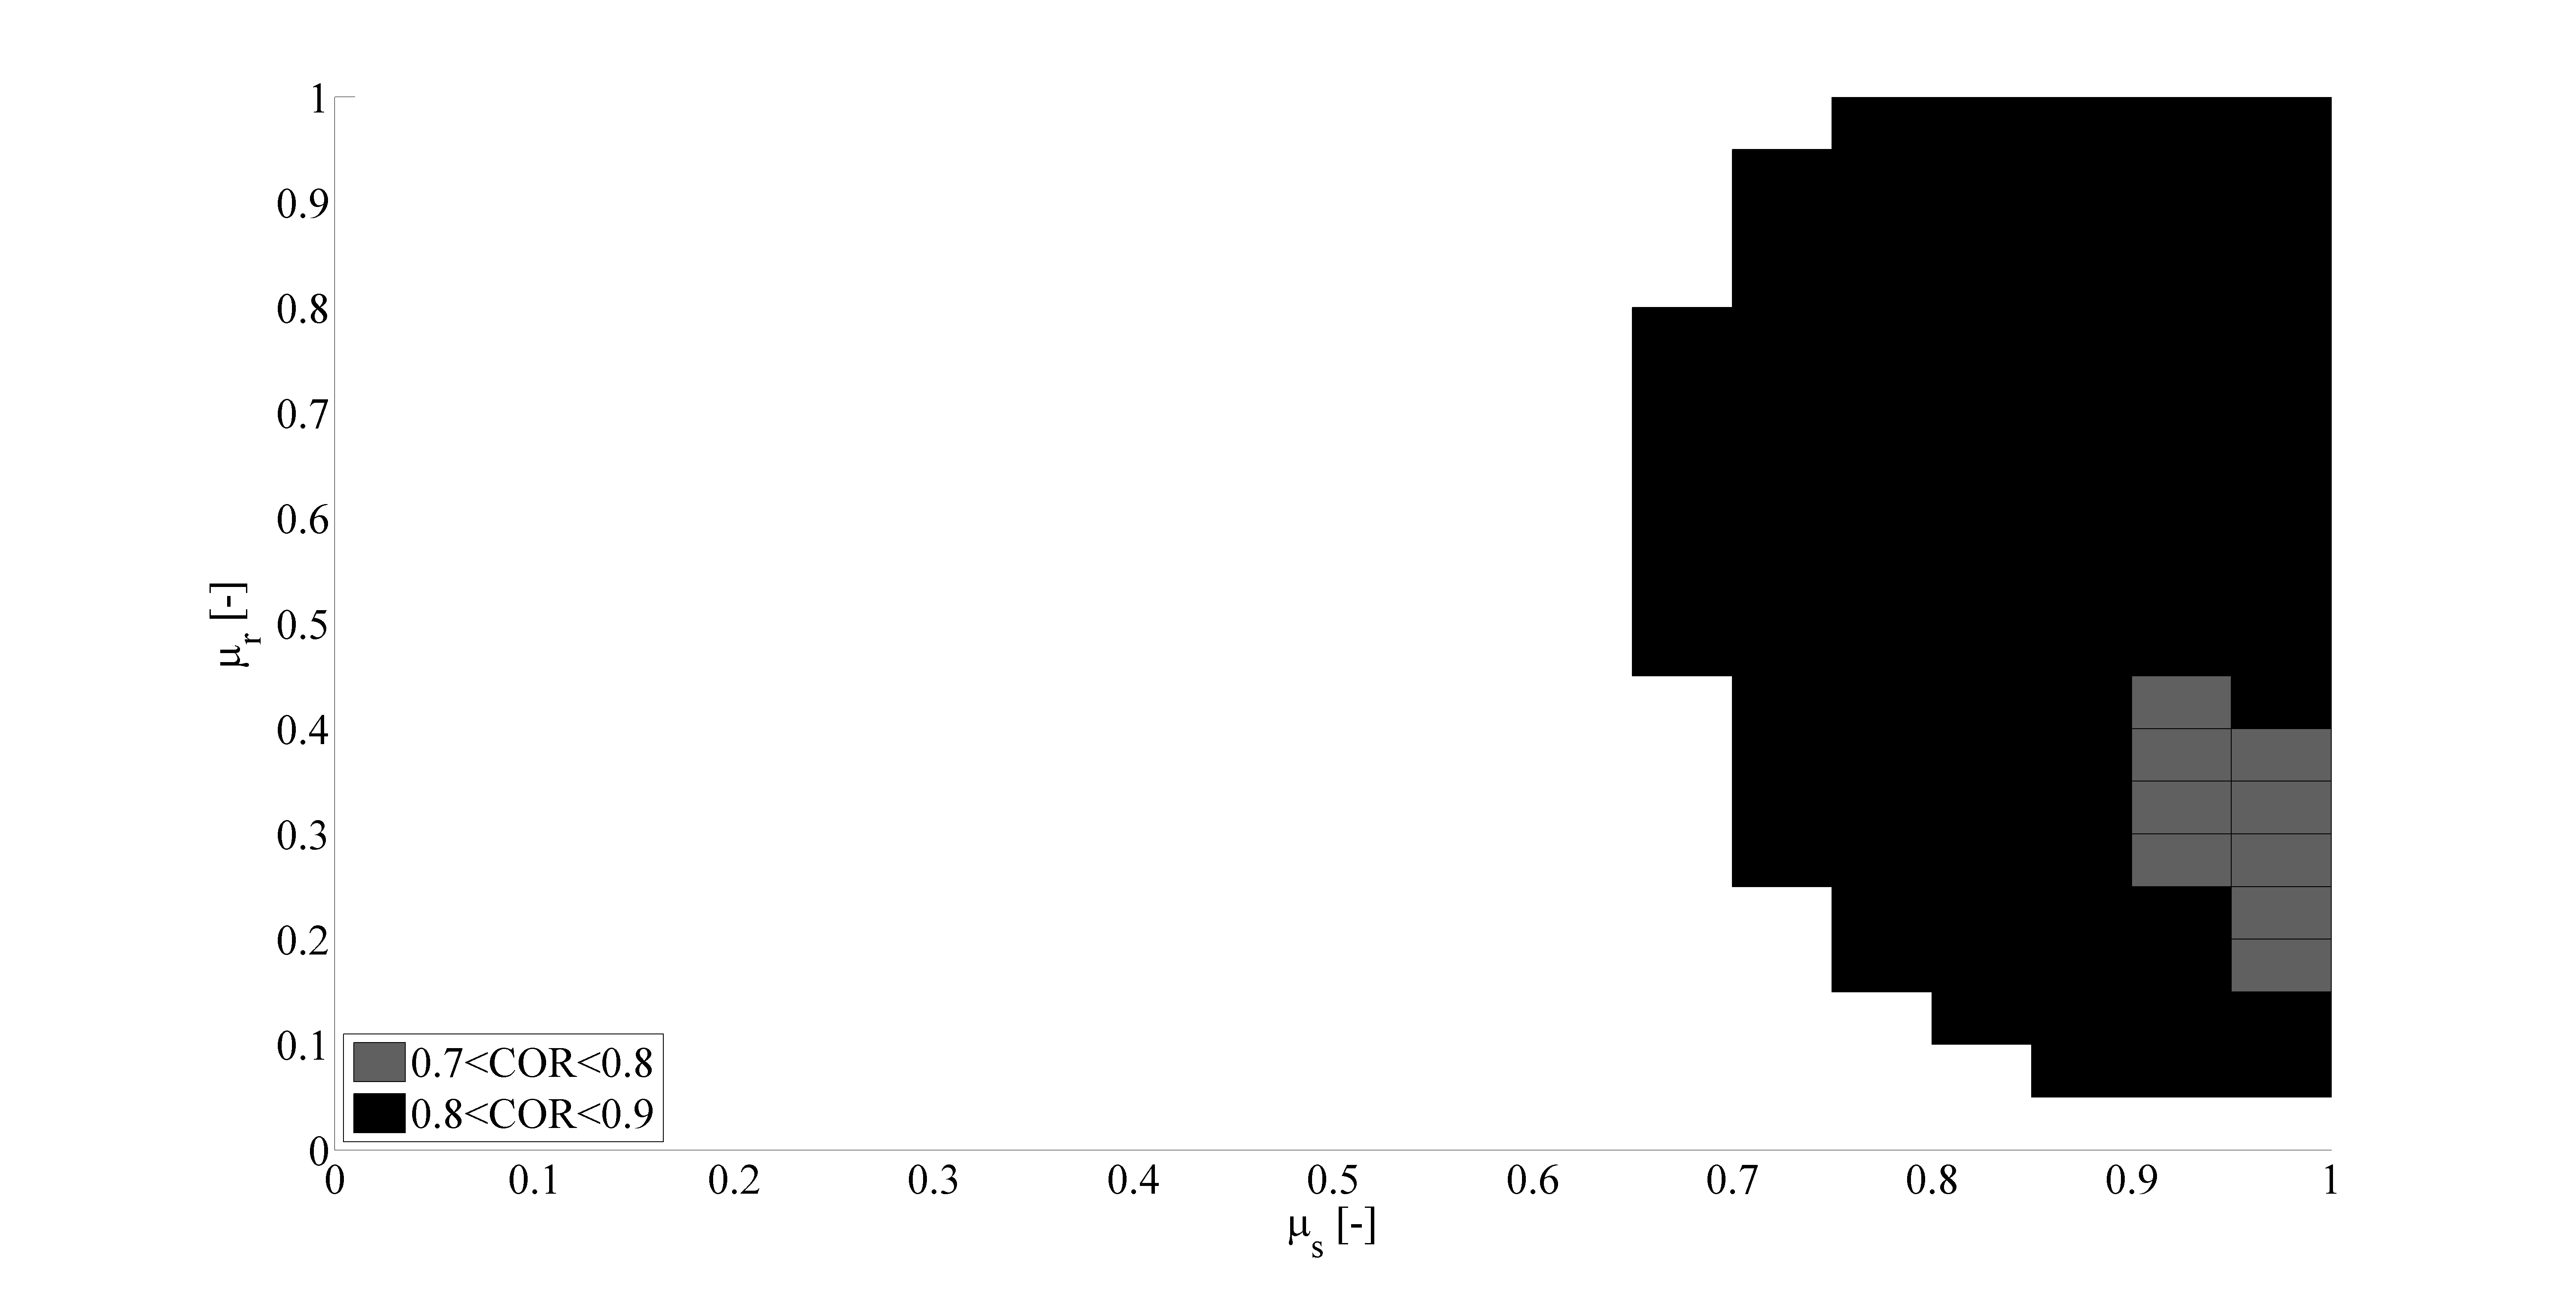
\includegraphics[width=.48\columnwidth]{images/030cloudpirker12schulze10070}
	  \label{fig:030cloudpirker12schulze10070}
  }
  \\
  \caption{Density plot comparison of SCT results.}
  \label{fig:080sctdensityplots}
\end{figure}

\subsection{Reliability Considerations}
\label{subsec:reliabilityconsiderations}

We tested the marked combinations
by modifying the experimental bulk values of the shear cell to further prove
the validity of the system.
We artificially decreased or increased the shear force, and thus \acs{mupsh} and
\acs{mush}, by a product coefficient ($P$), e.g. Eq. \ref{eq:pcoeff}:
\begin{equation}
\label{eq:pcoeff}
\mu_{psh, new} = \mu_{psh, old} \cdot P .
\end{equation}

First, we set it to $P=0.8$, and we obtained another
series of marked combinations ($MC2$).
It could be seen in the parameter space plot in Fig.
\ref{fig:026radarpirker08schulze10070} that the confidence range is narrower
than for $P=1.0$, while in the density plot in Fig. 
\ref{fig:159TileSCT10070p08sinterfine} the area
appears larger, although slightly less densely populated. Finally, for $P=1.2$
and its marked combinations ($MC3$) the parameter space plot in Fig.
\ref{fig:028radarpirker12schulze10070} shows a largely different confidence
range, while the density plot in Fig. \ref{fig:161TileSCT10070p12sinterfine} 
shows a smaller area. As expected, the procedure was highly sensitive to
variations in the experimental data.
Our approach could therefore be used
for a wide range of bulk materials.\\

\subsection{AoR results}
\label{subsec:aorresults}

We then processed the random combinations with the \acs{AoR} \acs{ANN}. In Fig.
\ref{fig:031radarpirker1aor} the parameter space plot for the same criteria as
before could be seen.
In accordance with theory (Wensrich and Katterfeld \cite{RefWorks:87}), in a simulation dominated
by rolling particles, the coefficient of rolling friction has the maximum
influence. \\
\begin{figure}[htbp]
\centering 
  \subfloat[Parameter space plot, $AoR_{exp} = 38.85 ^\circ$.]{
	  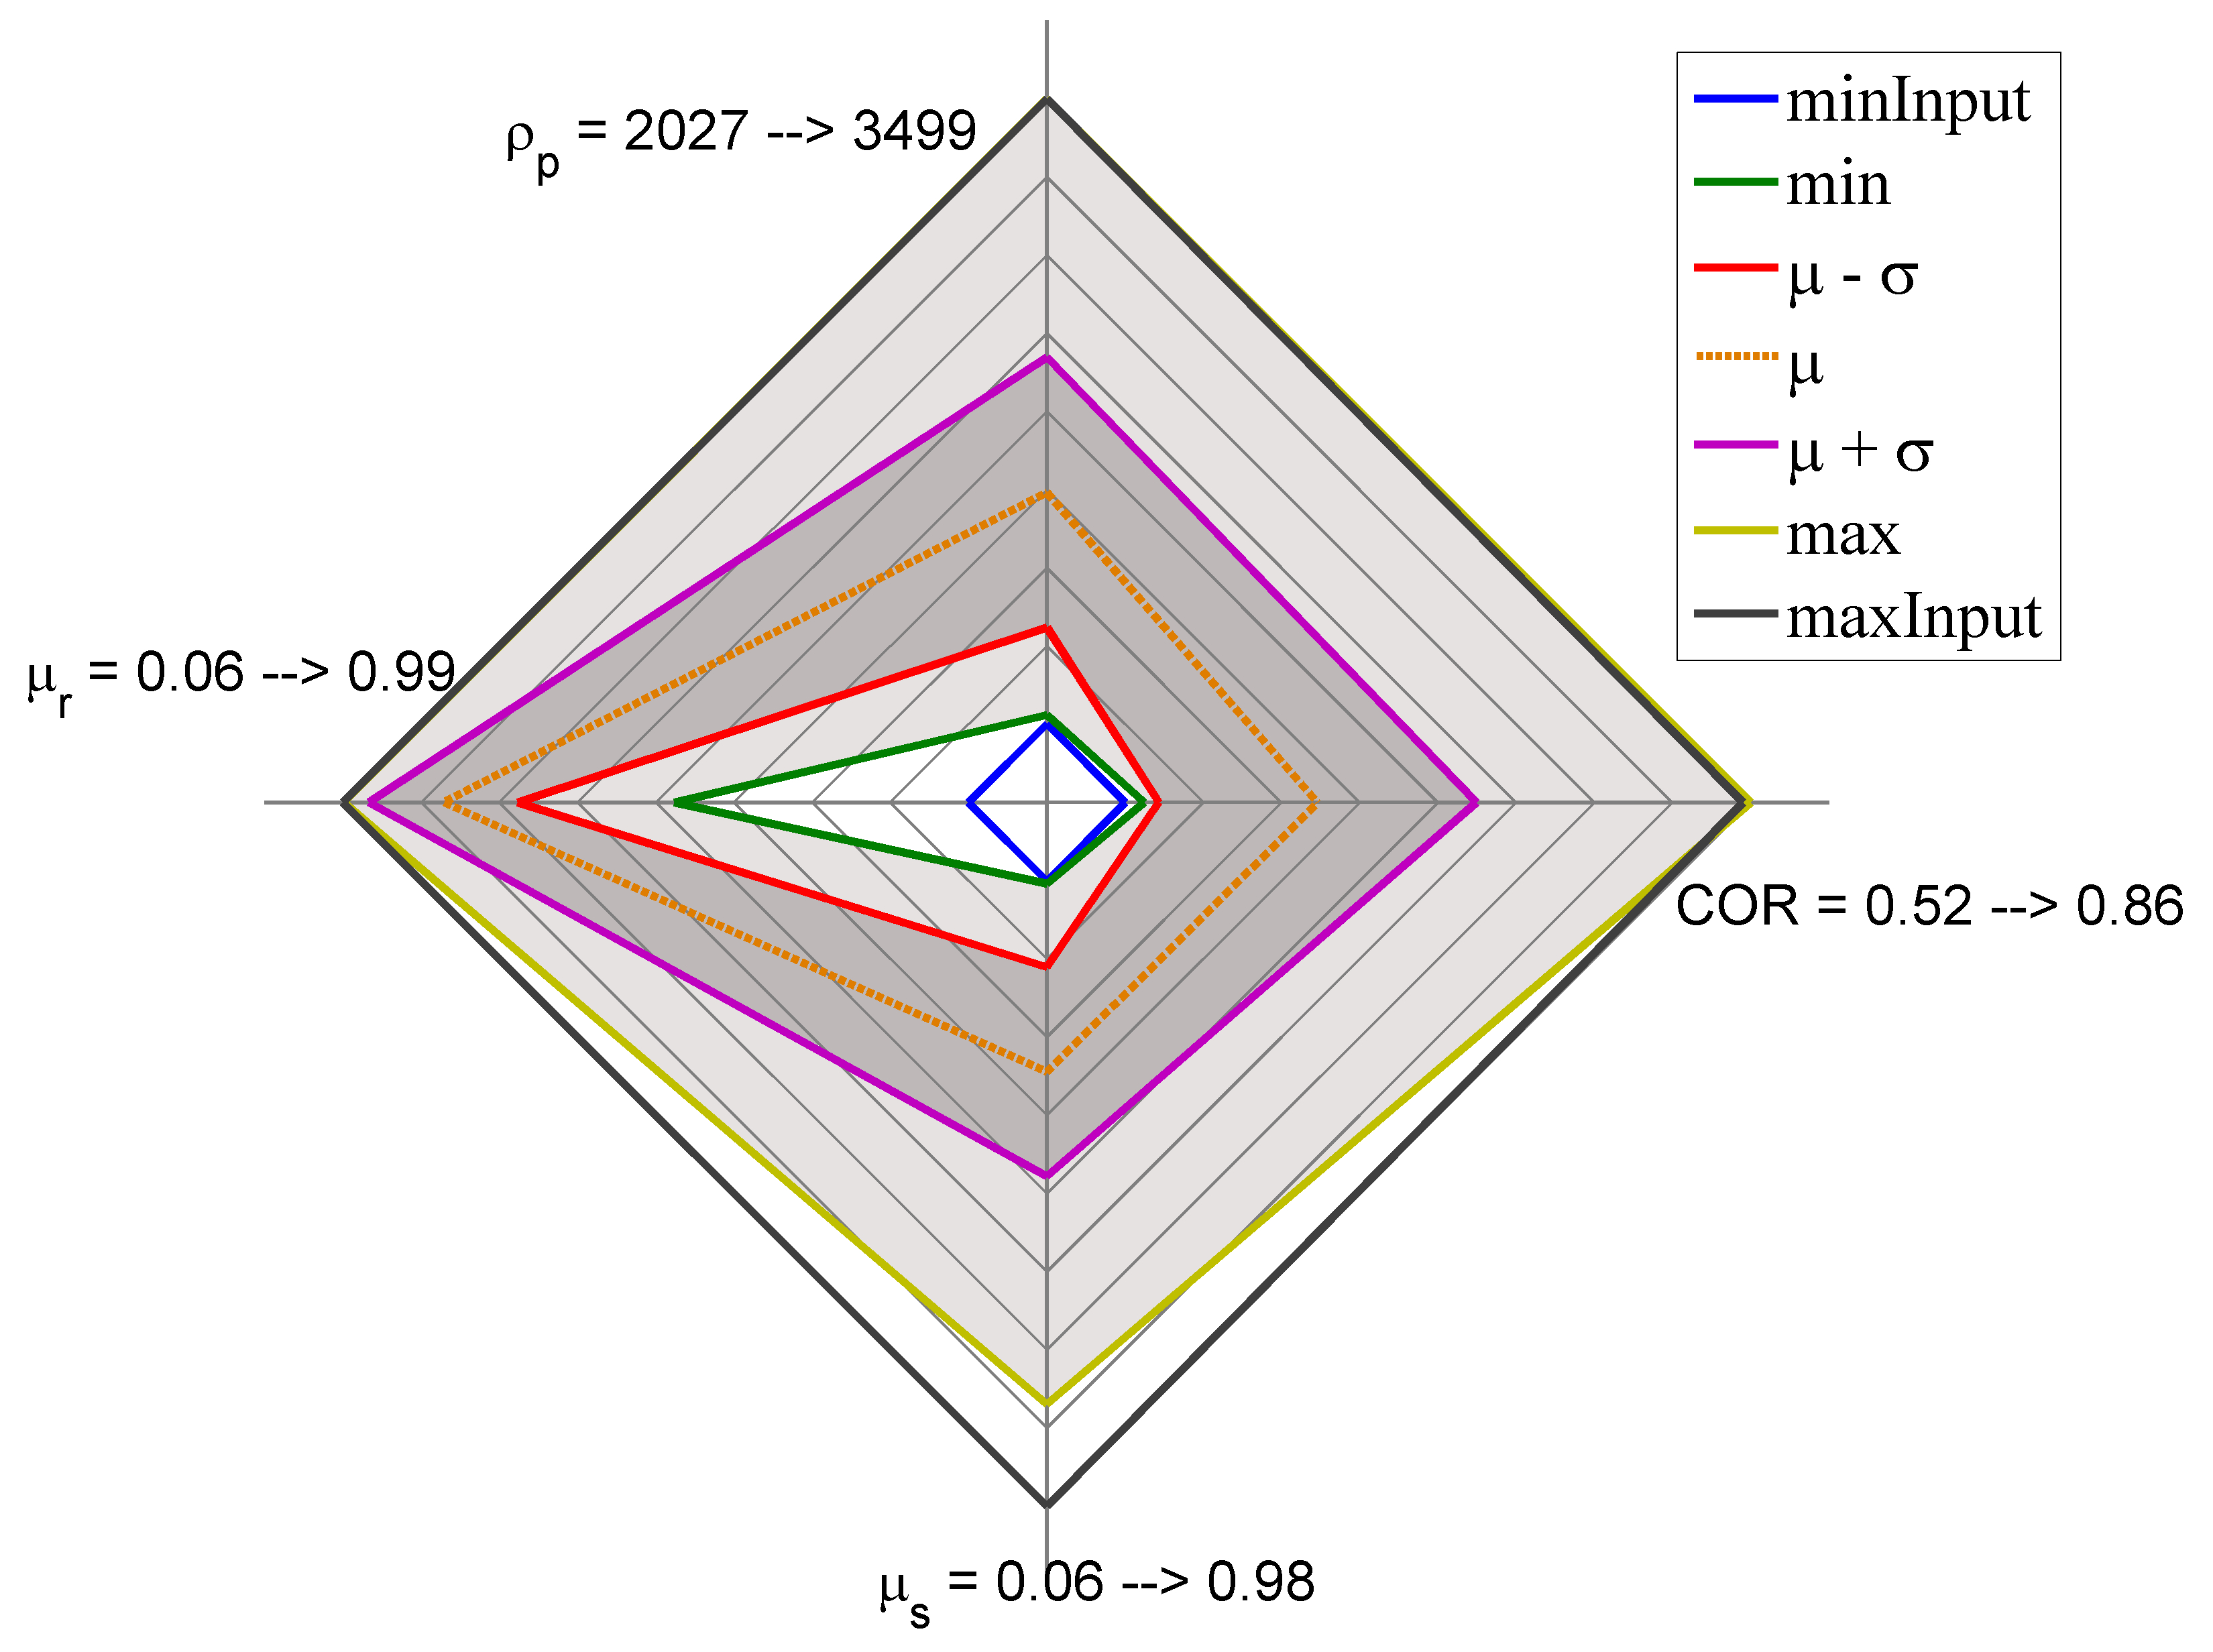
\includegraphics[width=.50\columnwidth]{images/031radarpirker1aor}
	  \label{fig:031radarpirker1aor}
  }
  \\
    \subfloat[Box plot, $AoR_{exp} = 38.85 ^\circ$.]{
	  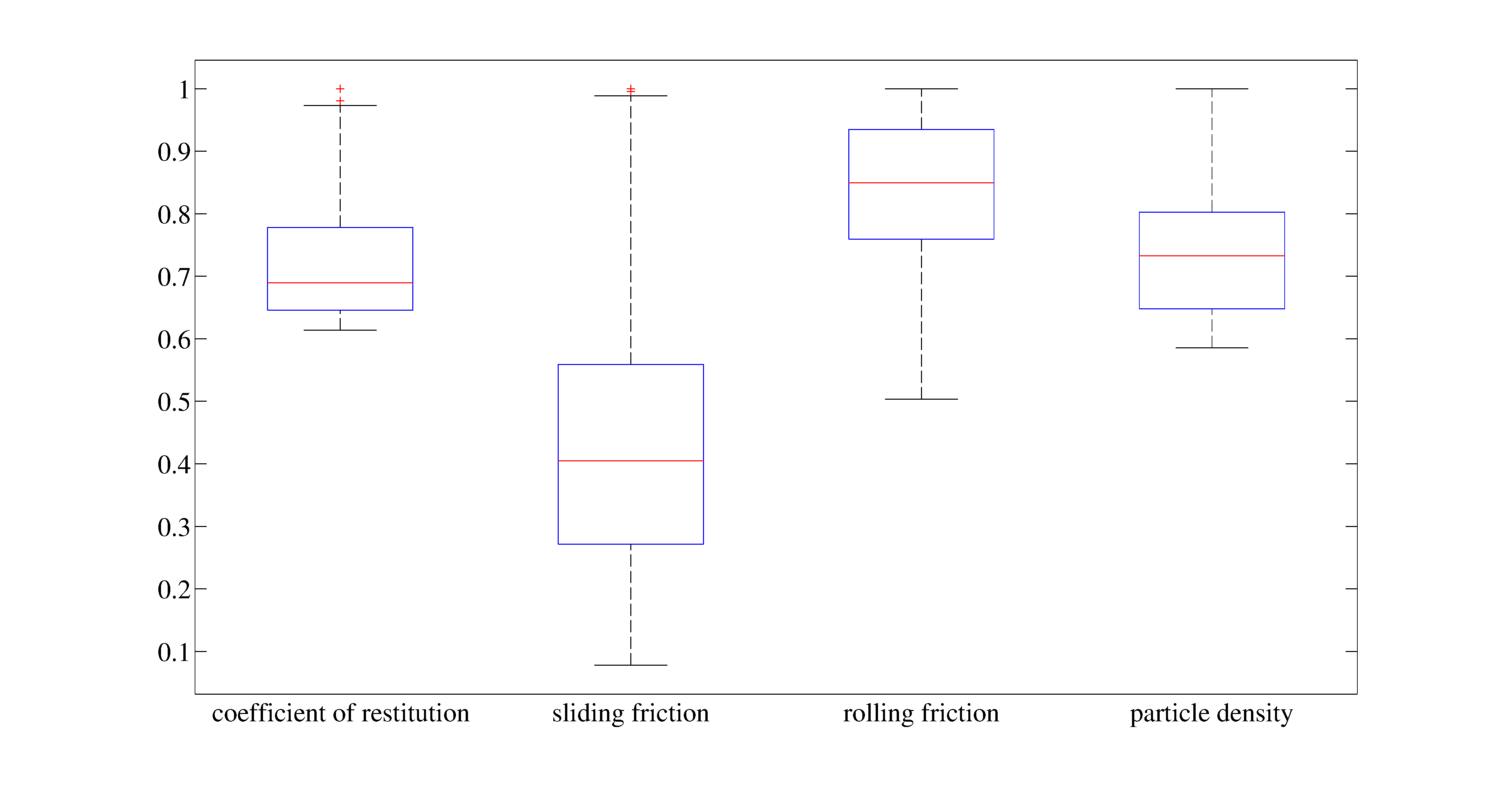
\includegraphics[width=.60\columnwidth]{images/076aorboxplot}
	  \label{fig:076aorboxplot}
  }
  \\
    \subfloat[Density plot plot, $AoR_{exp} = 38.85
        ^\circ$.]{
	  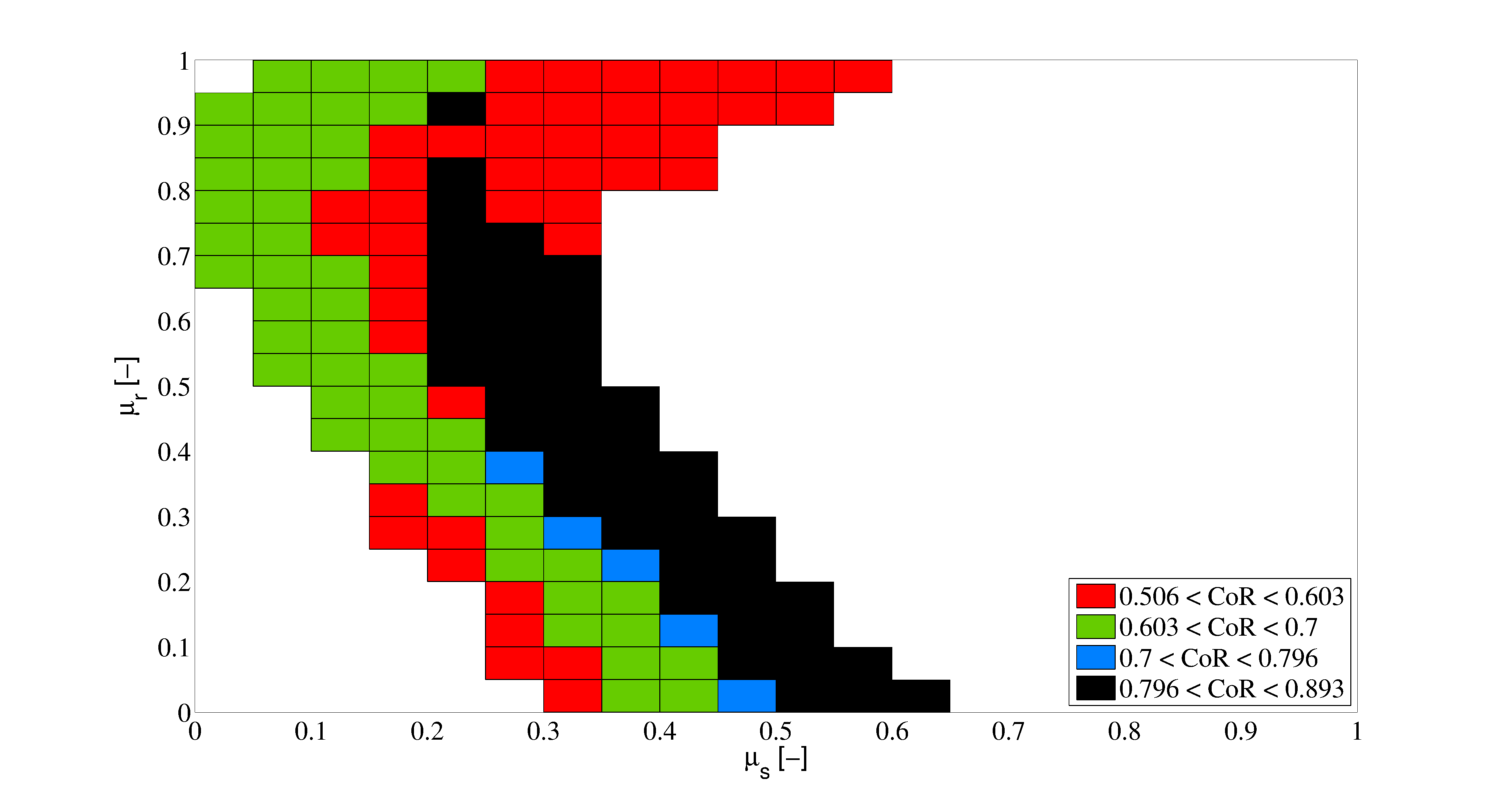
\includegraphics[width=.60\columnwidth]{images/162TileAORsinterfine}
	  \label{fig:162TileAORsinterfine}  }
  \\
  \caption[AoR valid values plots]{\acs{AoR} valid values plots. The valid
  values for the \acs{AoR} sinter fine test are shown in three different plots.
  The results are clearly different from the \acs{SCT} test and the \acs{mur}
  is the most relevant parameter.}
  \label{fig:207aorparameterspaceplots}
\end{figure}
%************************************************
% \begin{table}[h]
\centering
\begin{tabular}{cccccc}
\hline
$\sigma_n$ (Pa) & $\tau$ (Pa) & $\mu_{psh}$ (-) & $\tau_{\%}$ (\%) &
$\mu_{sh}$ (-) & $\rho_b$ (kg/m3) \\
\hline
    1068  & 1059  & 0.9916 & 80 & 1.2333 & 1718 \\
    2069  & 1818  & 0.8787 & 80 & 0.9994 & 1759 \\
    10070 & 8232  & 0.8175 & 80 & 1.1712 & 1802 \\

\hline
\end{tabular}
\caption[Experimental results]{Experimental results. Values for three
load conditions}
\label{tab:05sinterTableExperimental}
\end{table}
% \info{one table for each material? here or in the polydispersity chapter?}

\subsection{Merge results}
\label{subsec:mergeresults}

Finally, we extracted from the $MC1$ values the \acs{AoR} \acs{ANN} behaviour
and compared it with the experimental one.
As could be seen in the parameter space plot in Fig.
\ref{fig:208mergeparameterspaceplots}, the confidence interval is very small,
indicating that all the parameters but the \acs{CoR} played an important role, 
and demonstrating the reliability of these parameter
combinations in representing the bulk behaviour.
From the initial 6,250,000 combinations, only 3,884 were valid (0.0621
\%), see Table \ref{tab:13DEMvalidvalues}.

\begin{table}[h]
\centering
\begin{tabular}{llccc}
\hline

          & type  & SSC & AoR   & SSC \& AoR \\
          \hline

    $\mu_s$ & mean  & 0.831 & 0.177 & 0.664 \\
    $[-]$   & std. dev. (SD) & 0.097 & 0.095 & 0.029 \\
          & range ($R$) & 0.9   & 0.9   & 0.9 \\
          & SD / R & 0.108 & 0.106 & 0.032 \\
          \hline
    $\mu_r$ & mean  & 0.692 & 0.830 & 0.916 \\
    $[-]$   & std. dev. (SD) & 0.215 & 0.193 & 0.042 \\
          & range ($R$) & 0.9   & 0.9   & 0.9 \\
          & SD / R & 0.239 & 0.214 & 0.046 \\
          \hline
              COR   & mean  & 0.708 & 0.590 & 0.590 \\
   $ [-]$   & std. dev. (SD) & 0.104 & 0.073 & 0.065 \\
          & range ($R$) & 0.4   & 0.4   & 0.4 \\
          & SD / R & 0.259 & 0.183 & 0.161 \\
          \hline
    $\rho_p$ & mean  & 2245.7 & 3192.8 & 2283.9 \\
    $[kg/m3]$ & std. dev. (SD) & 80.5  & 277.4 & 67.1 \\
          & range ($R$) & 1500  & 1500  & 1500 \\
          & SD / R & 0.054 & 0.185 & 0.045 \\
          \hline
    valid & number & 290203 & 816552 & 3884 \\
    combinations & [$\%$] & 4.64  & 13.06 & 0.06 \\  

\hline
\end{tabular}
\caption[DEM valid values]{DEM valid values. For each parameter we show the
valid parameters statistics in the two tests and in their intersection.
Finally, we show the number of valid parameters combinations over the total
(6250000).}
\label{tab:13DEMvalidvalues}
\end{table}
\begin{figure}[htbp]
\centering 
  \subfloat[Parameter space plot, $AoR_{exp} = 38.85 
        ^\circ$ \& \acs{SCT}: $\sigma_n=10070$ Pa.]{
	  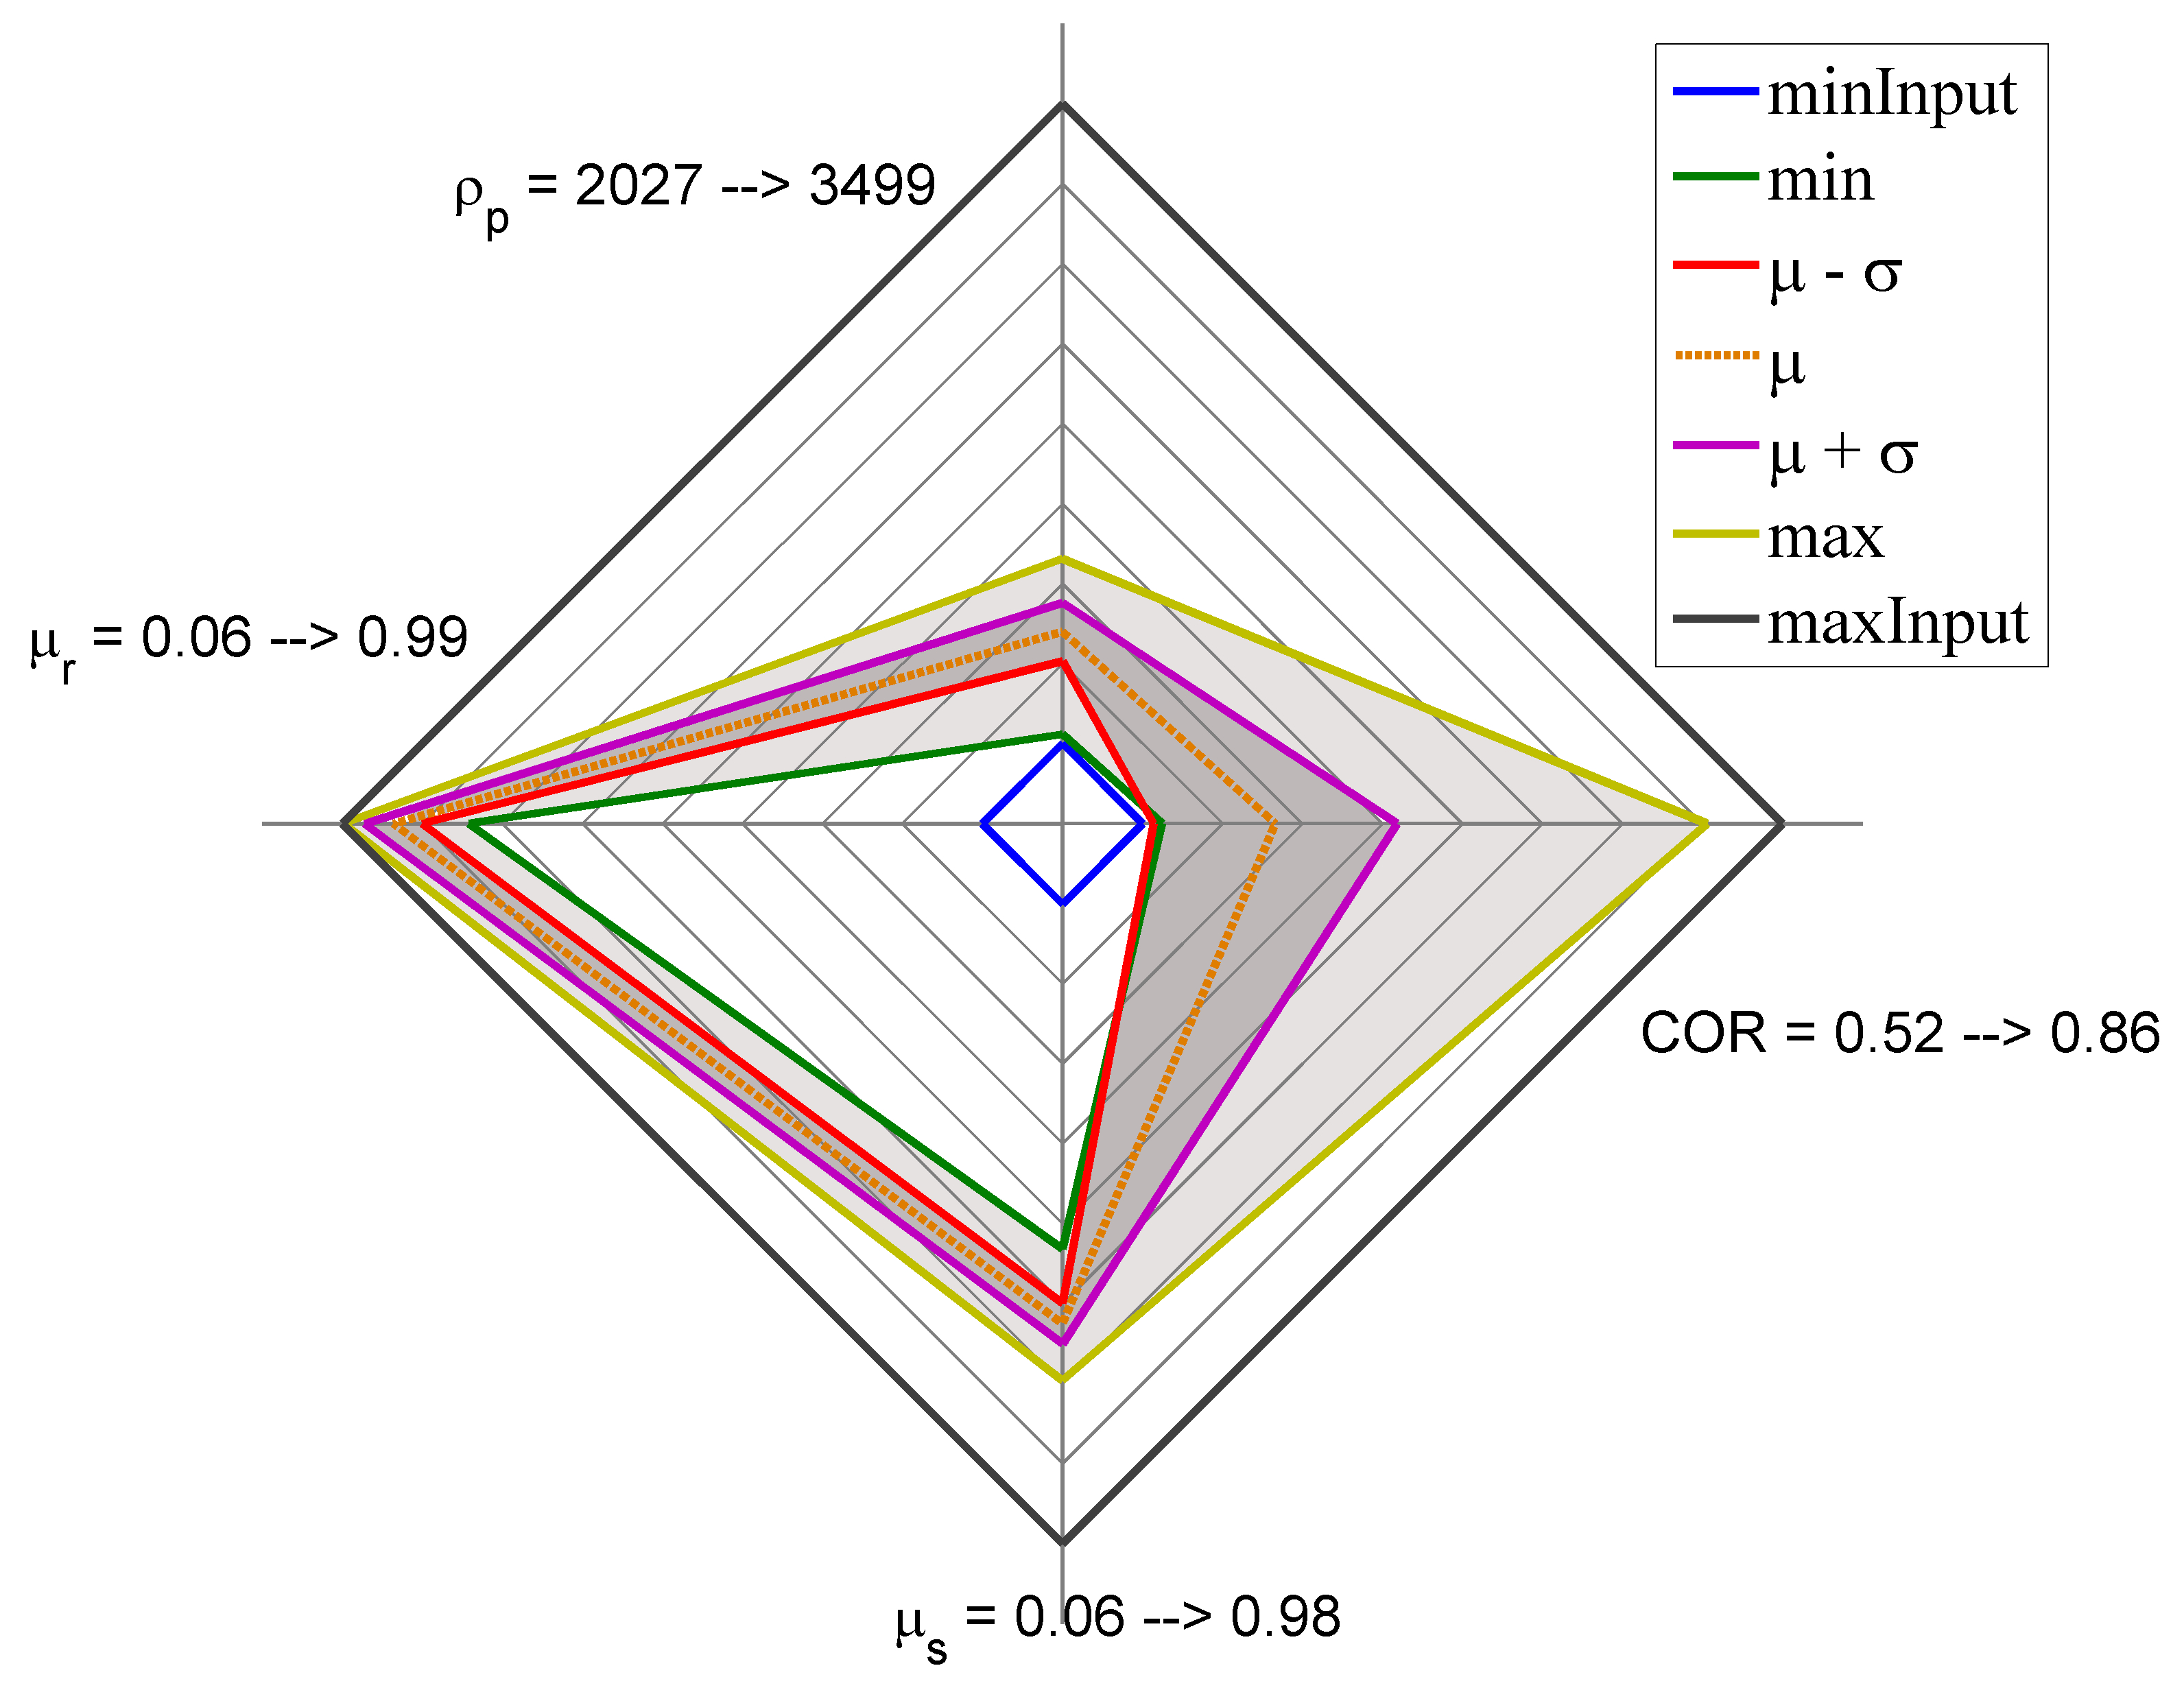
\includegraphics[width=.50\columnwidth]{images/033radarpirker1schulze10070aor}
	  \label{fig:033radarpirker1schulze10070aor}
  }
  \\
    \subfloat[Box plot, $AoR_{exp} = 38.85
        ^\circ$ \& \acs{SCT}: $\sigma_n=10070$ Pa.]{
	  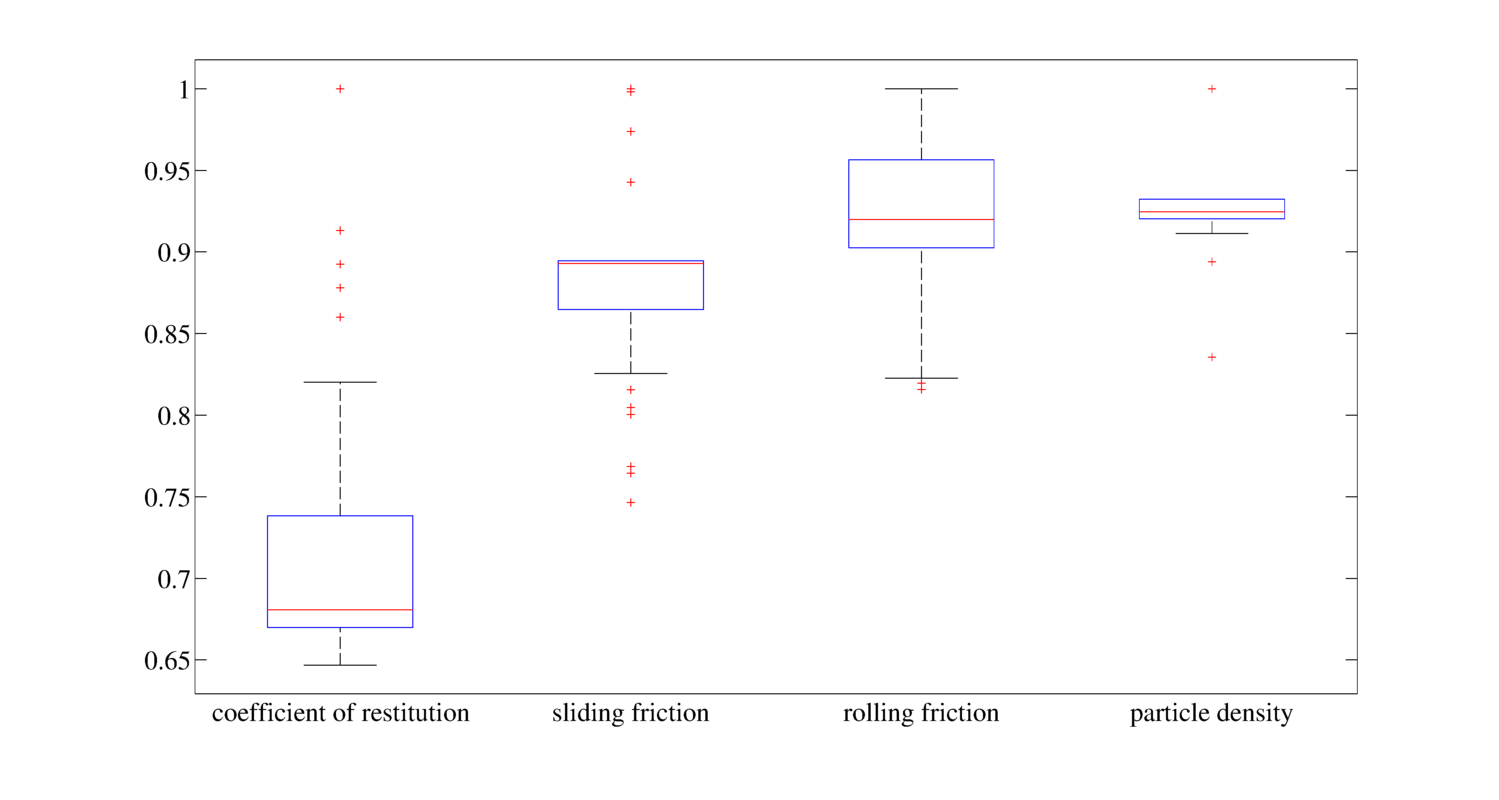
\includegraphics[width=.60\columnwidth]{images/078mergeboxplot}
	  \label{fig:078mergeboxplot}  }
  \\
  \subfloat[TIle plot, $AoR_{exp} = 38.85 
        ^\circ$ \& \acs{SCT}: $\sigma_n=10070$ Pa.]{
	  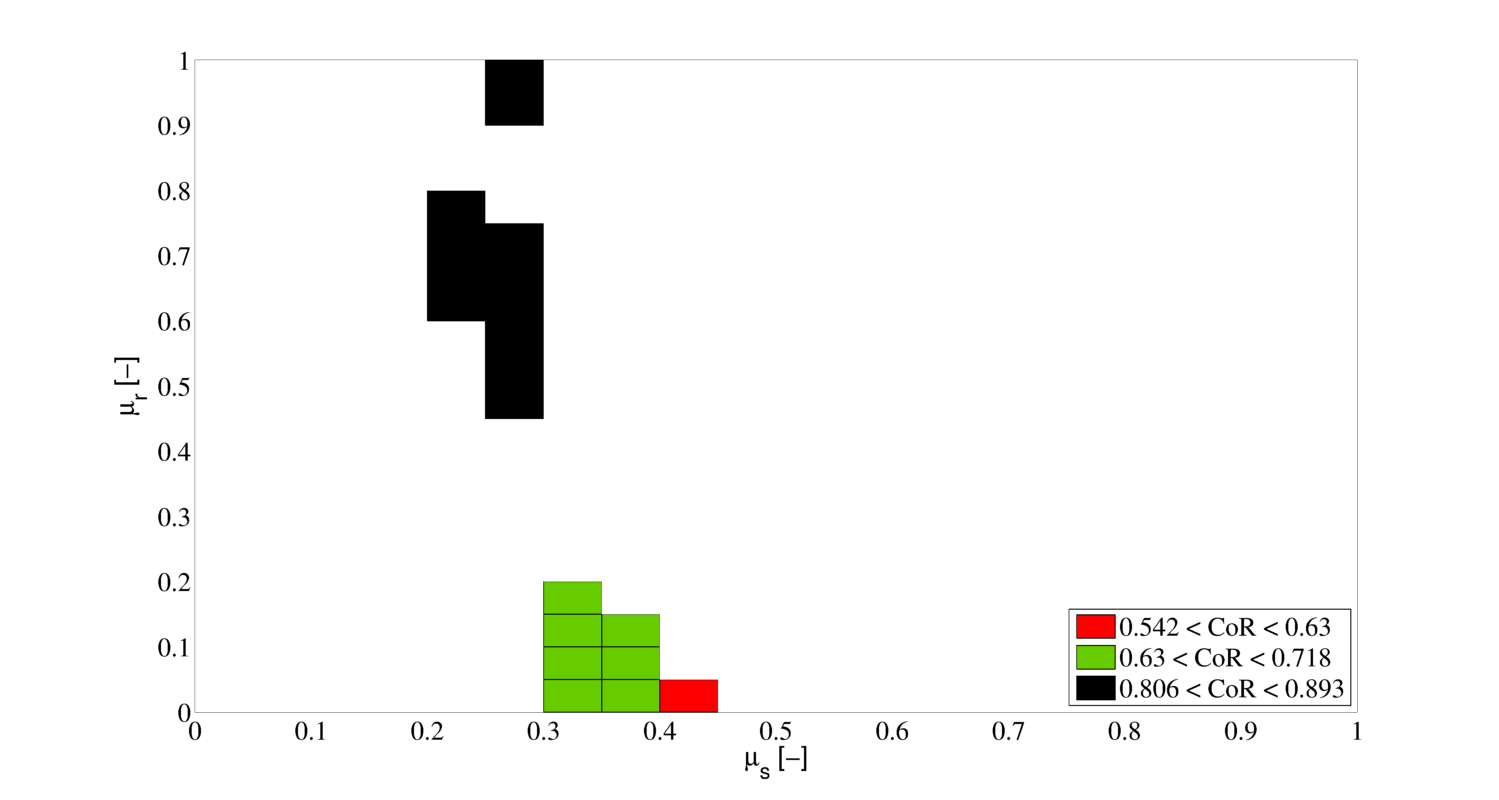
\includegraphics[width=.60\columnwidth]{images/206TileMixsinterfine_33}
	  \label{fig:206TileMixsinterfine_33}
  }
  \\  
  \caption{Merge parameter space plots.}
  \label{fig:208mergeparameterspaceplots}
\end{figure}


%************************************************
%************************************************

\section{Remaining Materials Characterization}
\label{sec:remainingmaterialscharacterization}

We later proceeded in further expanding the characterization by investigating
the values for the remaining materials.
Thus, we realized a limited number of simulations (620 \acs{SCT} simulations
and 180 \acs{AoR} simulations) with the particles distributions in Table
\ref{tab:19particlesizedistributions} and the stress conditions in Table
\ref{tab:21shearcell2}.\\
Together with the simulations already performed for sinter fine, we trained
additional \acs{ANNs} for the four bulk values involved.
Again, we extracted those with the maximum \acs{r2}.
The weights and biases for the \acs{muie} can be found in Table
\ref{tab:33weightsbiasesmuie}.
Similarly, weights and biases for the \acs{AoR} are in Table
\ref{tab:32weightsbiasesAOR}.

\begin{sidewaystable}[htbp] 
 \centering 
\begin{tabular}{l|ccccccccccccccc} 
 \hline 
   &    \multicolumn{15}{l}{Weights of connection between input and hidden layer}  \\ 
 Neurons & 1 &  2 &  3 &  4 &  5 &  6 &  7 &  8 & 9 & 10 & 11 & 12 & 13 & 14 & 15  \\ 
 \hline 
  & 0.407 &  -0.055 &  -1.384 &  0.616 &  -0.436 &  -1.082 &  -0.155 &  0.667 &  -0.071  &  -0.567 &  1.388 &  -0.367 &  0.796 &  -0.815 &  1.607 \\ 
  & 0.242 &  -1.367 &  -1.057 &  -1.475 &  1.112 &  0.049 &  -0.002 &  0.688 &  0.517  &  1.395 &  0.009 &  -1.091 &  0.845 &  0.163 &  -0.122 \\ 
  & -0.045 &  0.866 &  0.026 &  0.012 &  0.277 &  0.221 &  -0.008 &  0.358 &  0.473  &  0.037 &  -0.004 &  -0.405 &  -0.507 &  -0.154 &  -0.170 \\ 
  & 0.803 &  0.001 &  -0.158 &  -0.039 &  0.491 &  -0.255 &  0.779 &  -0.004 &  -0.734  &  -0.339 &  -0.257 &  -0.862 &  -0.014 &  -1.375 &  0.403 \\ 
  & -1.984 &  -0.734 &  0.533 &  0.182 &  0.754 &  0.861 &  -0.627 &  0.790 &  -0.505  &  0.048 &  -0.262 &  0.093 &  0.160 &  0.810 &  -0.038 \\ 
  & 0.092 &  -0.320 &  -0.327 &  -0.046 &  -0.596 &  0.175 &  0.805 &  -1.232 &  1.130  &  0.601 &  0.303 &  0.505 &  -1.295 &  0.245 &  -0.347 \\ 
  & -0.285 &  -0.094 &  1.291 &  -0.007 &  -0.352 &  -0.947 &  0.077 &  0.452 &  0.557  &  -0.245 &  -0.096 &  -1.089 &  0.297 &  -1.300 &  -0.340 \\ 
  & -0.058 &  0.250 &  -0.061 &  -0.147 &  -0.864 &  0.893 &  0.422 &  0.690 &  -0.246  &  -0.239 &  -0.036 &  0.569 &  0.448 &  -0.639 &  1.007 \\ 
\hline 
   &    \multicolumn{15}{l}{Weights of connection between hidden and output layer}  \\ 
  & 1.114 &  -0.026 &  -0.156 &  -0.348 &  -0.024 &  -0.024 &  -0.172 &  0.065 &  -0.085  &  -0.121 &  0.404 &  -0.057 &  -0.083 &  -0.117 &  0.009 \\ 
\hline 
   &    \multicolumn{15}{l}{Biases of hidden layer}  \\ 
  & -2.744 &  -1.815 &  1.032 &  -1.501 &  0.845 &  0.385 &  0.324 &  -0.113 &  -0.567  &  -0.573 &  1.114 &  -0.982 &  1.564 &  -1.068 &  1.630 \\ 
\hline 
   &    \multicolumn{15}{l}{Biases of output layer}  \\ 
 &    \multicolumn{15}{c}{0.151}  \\ 
\hline 
 \end{tabular} 
\caption[Weights and biases table for coefficient of internal friction]{Weights and biases table for coefficient of internal friction.} 
\label{tab:33weightsbiasesmuie} 
\end{sidewaystable}
\begin{table}[htbp] 
 \centering 
\begin{tabular}{l|ccccccccc} 
 \hline 
   &    \multicolumn{9}{l}{Weights of connection between input and hidden layer}  \\ 
 Neurons & 1 &  2 &  3 &  4 &  5 &  6 &  7 &  8 & 9 \\ 
 \hline 
  & 1.312 &  -1.389 &  -1.470 &  0.368 &  -0.259 &  -0.014 &  3.356 &  -0.692 &  0.446 \\ 
  & -1.729 &  0.699 &  -0.660 &  0.622 &  0.769 &  1.156 &  0.488 &  -0.656 &  0.601 \\ 
  & -0.539 &  -1.052 &  0.228 &  -0.535 &  -0.180 &  -0.870 &  -0.149 &  0.672 &  -0.721 \\ 
  & 0.029 &  -0.100 &  0.357 &  -1.181 &  1.490 &  -0.777 &  0.016 &  -0.824 &  -0.620 \\ 
  & -0.022 &  -0.173 &  0.597 &  1.444 &  0.736 &  1.141 &  -0.029 &  -1.045 &  -0.859 \\ 
  & 0.192 &  -0.239 &  0.320 &  -0.151 &  0.357 &  -0.464 &  -0.042 &  -0.759 &  0.735 \\ 
\hline 
   &    \multicolumn{9}{l}{Weights of connection between hidden and output layer}  \\ 
  & -0.512 &  0.242 &  -0.098 &  0.030 &  -0.068 &  -0.003 &  0.750 &  -0.013 &  -0.010 \\ 
\hline 
   &    \multicolumn{9}{l}{Biases of hidden layer}  \\ 
  & -2.204 &  1.678 &  0.999 &  -0.526 &  -0.294 &  -0.298 &  0.683 &  -1.631 &  2.343 \\ 
\hline 
   &    \multicolumn{9}{l}{Biases of output layer}  \\ 
 &    \multicolumn{9}{c}{-0.739}  \\ 
\hline 
 \end{tabular} 
\caption[Weights and biases table for AOR]{Weights and biases table for AOR.} 
\label{tab:32weightsbiasesAOR} 
\end{table}


\subsection{Coke coarse Characterization}
\label{subsec:cokecoarsecharacterization}

The valid values identified for the coke coarse can be found in Table
\ref{tab:25DEMvalidvaluescokecoarse}.\\
However, while the plots referring to the single test show reasonably narrow
confidence ranges, Fig. \ref{fig:197BoxMixcokecoarse_27} shows unreasonably
large valid ranges.
For comparison, in Fig. \ref{fig:198TileMixcokecoarse_27} only a tiny portion of
the density plot is colored.
In fact, this means that the choice of valid values is limited, as Table
\ref{tab:25DEMvalidvaluescokecoarse} shows.
\begin{table}[htbp] 
 \centering 
\begin{tabular}{ll|cccc} 
 \hline 
 &    & SSC & SSC & AoR   & SSC \& AoR \\ 
 & $\sigma_n$  [Pa]  & 1000 & 2000 &    &  \\ 
 \hline 
\acs{mus} & mean & 0.611 & 0.582 & 0.541 & 0.456 \\ 
$(-)$ & std. dev. (SD) & 0.118 & 0.118 & 0.138 & 0.037 \\ 
 & range (\acs{R}) & 0.959 & 0.959 & 0.959 & 0.959 \\ 
 & SD / R & 0.123 & 0.123 & 0.144 & 0.038 \\ 
 \hline 
\acs{mur} & mean & 0.616 & 0.637 & 0.612 & 0.811 \\ 
$(-)$ & std. dev. (SD) & 0.231 & 0.194 & 0.263 & 0.081 \\ 
 & range (\acs{R}) & 0.950 & 0.950 & 0.950 & 0.950 \\ 
 & SD / R & 0.243 & 0.205 & 0.277 & 0.085 \\ 
 \hline 
\acs{CoR} & mean & 0.648 & 0.553 & 0.675 & 0.647 \\ 
$(-)$ & std. dev. (SD) & 0.057 & 0.048 & 0.123 & 0.023 \\ 
 & range (\acs{R}) & 0.387 & 0.387 & 0.387 & 0.387 \\ 
 & SD / R & 0.146 & 0.124 & 0.317 & 0.060 \\ 
 \hline 
\acs{rhop} & mean & 2748.1 & 2697.6 & 2747.7 & 2927.3 \\ 
$(-)$ & std. dev. (SD) & 413.4 & 410.0 & 409.3 & 388.4 \\ 
 & range (\acs{R}) & 1394.6 & 1394.6 & 1394.6 & 1394.6 \\ 
 & SD / R &  0.3 &  0.3 &  0.3 &  0.3 \\ 
 \hline 
valid & number & 193070 & 137121 & 654785 & 5481 \\ 
combinations & (\%)  & 0.06 & 0.04 & 0.21 & 0.00 \\ 
 \hline 
\end{tabular} 
\caption[Valid DEM values for coke coarse]{Valid DEM values for coke coarse. For
each parameter we show the valid parameter statistics in the the tests and in their intersection. Finally, we show the number of valid parameter combinations over the total (3062500).}
\label{tab:25DEMvalidvaluescokecoarse} 
\end{table}
\begin{figure}[htbp]
\centering 
  \subfloat[Box plot \acs{SCT}.]{
	  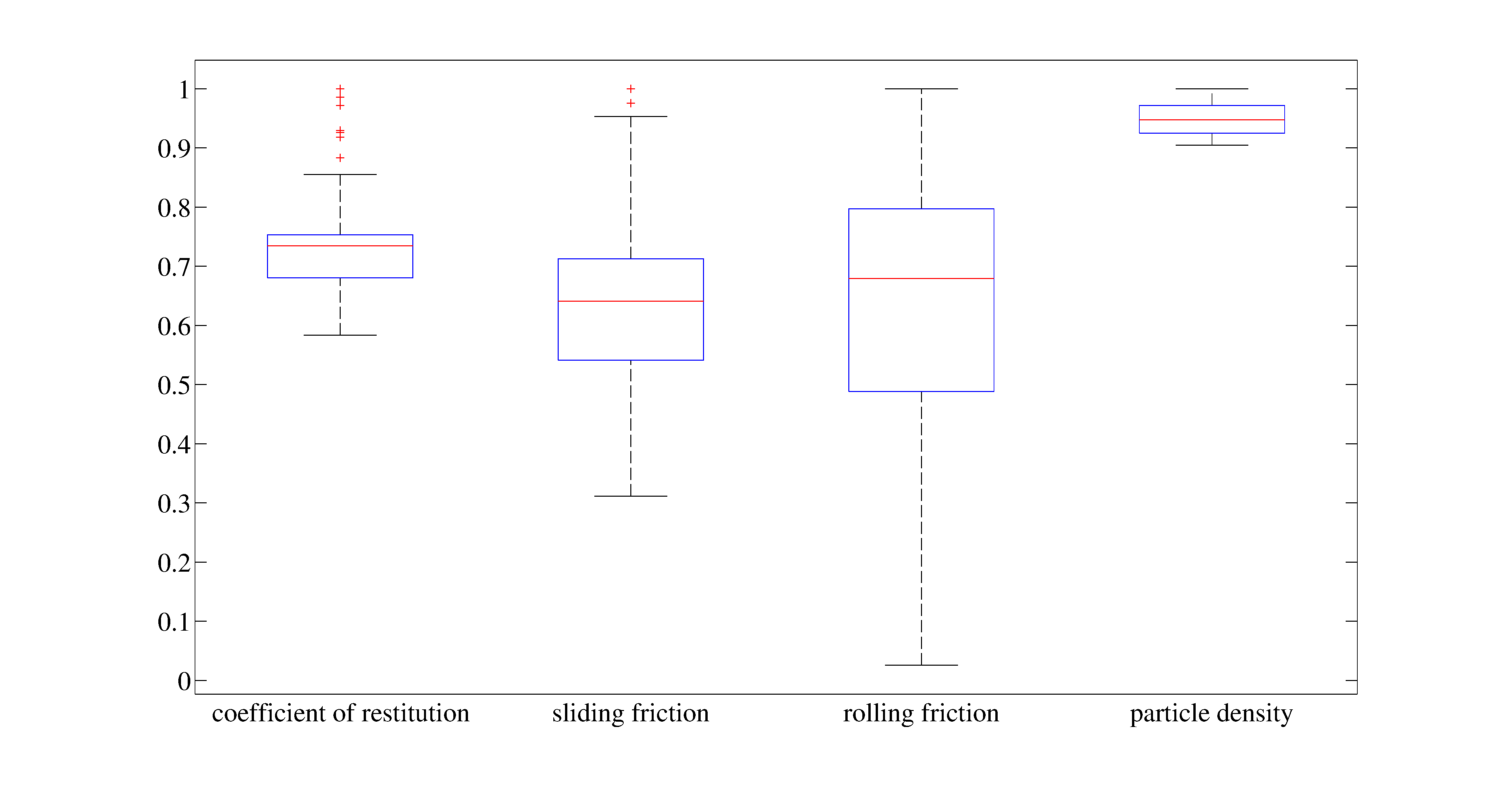
\includegraphics[width=.47\columnwidth]{images/166BoxSCTcokecoarsetest01coeffP1}
	  \label{fig:166BoxSCTcokecoarsetest01coeffP1}
  }
  \quad
  \subfloat[Density plot \acs{SCT}.]{
	  \includegraphics[width=.47\columnwidth]{images/172TileSCcokecoarsetest01coeffP1}
	  \label{fig:172TileSCcokecoarsetest01coeffP1}
  }
  \\
    \subfloat[Box plot \acs{AoR}.]{
	  \includegraphics[width=.47\columnwidth]{images/177BoxAORcokecoarse}
	  \label{fig:177BoxAORcokecoarse}  }
  \quad
   \subfloat[Density plot \acs{AoR}.]{
	  \includegraphics[width=.47\columnwidth]{images/178TileAORcokecoarse}
	  \label{fig:178TileAORcokecoarse}  }
  \\
  \subfloat[Box plot intersection: \acs{AoR} \& \acs{SCT}.]{
	  \includegraphics[width=.47\columnwidth]{images/197BoxMixcokecoarse_27}
	  \label{fig:197BoxMixcokecoarse_27}
  }
  \quad  
    \subfloat[Density plot intersection: \acs{AoR} \& \acs{SCT}.]{
	  \includegraphics[width=.47\columnwidth]{images/198TileMixcokecoarse_27}
	  \label{fig:198TileMixcokecoarse_27}
  }
  \\    
  \caption[Coke coarse]{Coke coarse. The valid values for the \acs{SCT} and
  \acs{AoR} tests are shown, together with the merge values, valid for both.
  The plots referring to the single test show reasonably narrow confidence
  ranges, while Fig. \ref{fig:197BoxMixcokecoarse_27} shows unreasonably large
  valid ranges. See Section \ref{sec:remainingmaterialscharacterization} for
  the interpretation.}
  \label{fig:209boxplotscokecoarse}
\end{figure}
%\begin{figure}[htbp]
\centering 
  \subfloat[\acs{SCT}.]{
	  \includegraphics[width=.60\columnwidth]{images/172TileSCcokecoarsetest01coeffP1}
	  \label{fig:172TileSCcokecoarsetest01coeffP1}
  }
  \\
    \subfloat[\acs{AoR}.]{
	  \includegraphics[width=.60\columnwidth]{images/178TileAORcokecoarse}
	  \label{fig:178TileAORcokecoarse}  }
  \\
  \subfloat[Intersection: \acs{AoR} \& \acs{SCT}.]{
	  \includegraphics[width=.60\columnwidth]{images/198TileMixcokecoarse_27}
	  \label{fig:198TileMixcokecoarse_27}
  }
  \\  
  \caption{Density plot plots coke coarse.}
  \label{fig:210tileplotscokecoarse}
\end{figure}


\subsection{Coke fine Characterization}
\label{subsec:cokefinecharacterization}

The range of valid values for coke is even narrower than that for the coke
coarse, see Fig. \ref{tab:211boxplotscokefine} and
Fig. \ref{fig:167BoxSCTcokefinetest02coeffP1}.
The final results can be read in Table \ref{tab:26DEMvalidvaluescokefine}.\\
Regrettably, considerations similar to those in Section
\ref{subsec:cokecoarsecharacterization} can be formulated for the intersation
box plot.
Fig. \ref{fig:192TileMixcokefine_3} shows the valid values.

\begin{table}[htbp] 
 \centering 
\begin{tabular}{ll|ccccc} 
 \hline 
 &    & SSC & SSC & SSC & AoR   & SSC \& AoR \\ 
 & $\sigma_n$  [Pa]  & 1000 & 2000 & 5000 &   &  \\ 
 \hline 
\acs{mus} & mean & 0.216 & 0.151 & 0.173 & 0.541 & 0.256 \\ 
$(-)$ & std. dev. (SD) & 0.028 & 0.026 & 0.023 & 0.138 & 0.017 \\ 
 & range (\acs{R}) & 0.959 & 0.959 & 0.959 & 0.959 & 0.959 \\ 
 & SD / R & 0.029 & 0.027 & 0.024 & 0.144 & 0.018 \\ 
 \hline 
\acs{mur} & mean & 0.310 & 0.330 & 0.229 & 0.612 & 0.535 \\ 
$(-)$ & std. dev. (SD) & 0.139 & 0.139 & 0.215 & 0.263 & 0.053 \\ 
 & range (\acs{R}) & 0.950 & 0.950 & 0.950 & 0.950 & 0.950 \\ 
 & SD / R & 0.146 & 0.146 & 0.226 & 0.277 & 0.056 \\ 
 \hline 
\acs{CoR} & mean & 0.687 & 0.689 & 0.808 & 0.675 & 0.586 \\ 
$(-)$ & std. dev. (SD) & 0.125 & 0.122 & 0.090 & 0.123 & 0.057 \\ 
 & range (\acs{R}) & 0.387 & 0.387 & 0.387 & 0.387 & 0.387 \\ 
 & SD / R & 0.322 & 0.314 & 0.234 & 0.317 & 0.148 \\ 
 \hline 
\acs{rhop} & mean & 2770.6 & 2758.0 & 2358.5 & 2747.7 & 2544.5 \\ 
$(-)$ & std. dev. (SD) & 406.2 & 404.3 & 289.2 & 409.3 & 373.5 \\ 
 & range (\acs{R}) & 1394.6 & 1394.6 & 1394.6 & 1394.6 & 1394.6 \\ 
 & SD / R &  0.3 &  0.3 &  0.2 &  0.3 &  0.3 \\ 
 \hline 
valid & number & 122110 & 136095 & 8767 & 654785 & 2718 \\ 
combinations & (\%)  & 0.04 & 0.04 & 0.00 & 0.21 & 0.00 \\ 
 \hline 
\end{tabular} 
\caption[Valid DEM values for coke fine]{Valid DEM values for coke fine. For
each parameter we show the valid parameter statistics in the the tests and in their intersection. Finally, we show the number of valid parameter combinations over the total (3062500).}
\label{tab:26DEMvalidvaluescokefine} 
\end{table}
\begin{figure}[htbp]
\centering 
  \subfloat[\acs{SCT}.]{
	  \includegraphics[width=.60\columnwidth]{images/167BoxSCTcokefinetest02coeffP1}
	  \label{fig:167BoxSCTcokefinetest02coeffP1}
  }
  \\
    \subfloat[\acs{AoR}.]{
	  \includegraphics[width=.60\columnwidth]{images/179BoxAORcokefine}
	  \label{fig:179BoxAORcokefine}  }
  \\
  \subfloat[Intersection: \acs{AoR} \& \acs{SCT}.]{
	  \includegraphics[width=.60\columnwidth]{images/191BoxMixcokefine_3}
	  \label{fig:191BoxMixcokefine_3}
  }
  \\  
  \caption{Box plots coke fine.}
  \label{fig:211boxplotscokefine}
\end{figure}
%\begin{figure}[htbp]
\centering 
  \subfloat[\acs{SCT}.]{
	  \includegraphics[width=.60\columnwidth]{images/173TileSCcokefinetest02coeffP1-2}
	  \label{fig:173TileSCcokefinetest02coeffP1-2}
  }
  \\
    \subfloat[\acs{AoR}.]{
	  \includegraphics[width=.60\columnwidth]{images/180TileAORcokefine}
	  \label{fig:180TileAORcokefine}  }
  \\
  \subfloat[Intersection: \acs{AoR} \& \acs{SCT}.]{
	  \includegraphics[width=.60\columnwidth]{images/192TileMixcokefine_3}
	  \label{fig:192TileMixcokefine_3}
  }
  \\  
  \caption{Density plot plots coke fine.}
  \label{fig:212tileplotscokefine}
\end{figure}


\subsection{Iron ore coarse Characterization}
\label{subsec:ironorecoarsecharacterization}

The iron ore coarse is subject to the identical considerations of coke coarse,
shown in Section \ref{subsec:cokecoarsecharacterization}.
Fig. \ref{fig:213boxplotsironorecoarse} and Fig.
\ref{fig:214tileplotsironorecoarse}, together with Table
\ref{tab:27DEMvalidvaluesironorecoarse}, show the final values.

\begin{table}[htbp] 
 \centering 
\begin{tabular}{ll|ccccc} 
 \hline 
 &    & SSC & SSC & SSC & AoR   & SSC \& AoR \\ 
 & $\sigma_n$  [Pa]  & 1000 & 2000 & 5000 &   &  \\ 
 \hline 
\acs{mus} & mean & 0.852 & 0.439 & 0.557 & 0.459 & 0.461 \\ 
$(-)$ & std. dev. (SD) & 0.106 & 0.057 & 0.102 & 0.149 & 0.029 \\ 
 & range (\acs{R}) & 0.959 & 0.959 & 0.959 & 0.959 & 0.959 \\ 
 & SD / R & 0.111 & 0.059 & 0.106 & 0.155 & 0.031 \\ 
 \hline 
\acs{mur} & mean & 0.605 & 0.577 & 0.675 & 0.612 & 0.642 \\ 
$(-)$ & std. dev. (SD) & 0.242 & 0.237 & 0.176 & 0.253 & 0.064 \\ 
 & range (\acs{R}) & 0.950 & 0.950 & 0.950 & 0.950 & 0.950 \\ 
 & SD / R & 0.255 & 0.249 & 0.185 & 0.266 & 0.067 \\ 
 \hline 
\acs{CoR} & mean & 0.697 & 0.559 & 0.541 & 0.662 & 0.577 \\ 
$(-)$ & std. dev. (SD) & 0.041 & 0.068 & 0.036 & 0.123 & 0.031 \\ 
 & range (\acs{R}) & 0.387 & 0.387 & 0.387 & 0.387 & 0.387 \\ 
 & SD / R & 0.107 & 0.176 & 0.092 & 0.317 & 0.079 \\ 
 \hline 
\acs{rhop} & mean & 2823.6 & 2692.3 & 2691.0 & 2755.0 & 2612.3 \\ 
$(-)$ & std. dev. (SD) & 408.9 & 410.9 & 410.0 & 408.4 & 405.9 \\ 
 & range (\acs{R}) & 1394.6 & 1394.6 & 1394.6 & 1394.6 & 1394.6 \\ 
 & SD / R &  0.3 &  0.3 &  0.3 &  0.3 &  0.3 \\ 
 \hline 
valid & number & 156816 & 119311 & 119330 & 784045 & 10006 \\ 
combinations & (\%)  & 0.05 & 0.04 & 0.04 & 0.26 & 0.00 \\ 
 \hline 
\end{tabular} 
\caption[Valid DEM values for ironorecoarse]{Valid DEM values for ironorecoarse. For each parameter we show the valid parameter statistics in the the tests and in their intersection. Finally, we show the number of valid parameter combinations over the total (3062500).} 
\label{tab:27DEMvalidvaluesironorecoarse} 
\end{table}
\begin{figure}[htbp]
\centering 
  \subfloat[Box plot \acs{SCT}.]{
	  \includegraphics[width=.47\columnwidth]{images/168BoxSCTironorecoarsetest01coeffP1}
	  \label{fig:168BoxSCTironorecoarsetest01coeffP1}
  }
  \quad
  \subfloat[Density plot \acs{SCT}.]{
	  \includegraphics[width=.47\columnwidth]{images/174TileSCironorecoarsetest01coeffP1}
	  \label{fig:174TileSCironorecoarsetest01coeffP1}
  }
  \\
    \subfloat[Box plot \acs{AoR}.]{
	  \includegraphics[width=.47\columnwidth]{images/181BoxAORironorecoarse}
	  \label{fig:181BoxAORironorecoarse}  }
  \quad
  \subfloat[Density plot \acs{AoR}.]{
	  \includegraphics[width=.47\columnwidth]{images/182TileAORironorecoarse}
	  \label{fig:182TileAORironorecoarse}  }
  \\
  \subfloat[Box plot intersection: \acs{AoR} \& \acs{SCT}.]{
	  \includegraphics[width=.47\columnwidth]{images/199BoxMixironorecoarse_28}
	  \label{fig:199BoxMixironorecoarse_28}
  }
  \quad
  \subfloat[Density plot intersection: \acs{AoR} \& \acs{SCT}.]{
	  \includegraphics[width=.47\columnwidth]{images/200TileMixironorecoarse_28}
	  \label{fig:200TileMixironorecoarse_28}
  }
  \\    
  \caption[Iron ore coarse valid values]{Iron ore coarse valid values. The valid
  values for the \acs{SCT} and \acs{AoR} tests are shown, together with the merge values, valid for both.
  The plots referring to the single test show reasonably narrow confidence
  ranges, while Fig. \ref{fig:199BoxMixironorecoarse_28} shows unreasonably large
  valid ranges. See Section \ref{sec:remainingmaterialscharacterization} for
  the interpretation.}
  \label{fig:213boxplotsironorecoarse}
\end{figure}
%%\begin{figure}[htbp]
%\centering 
%  \subfloat[\acs{SCT}.]{
%	  \includegraphics[width=.60\columnwidth]{images/174TileSCironorecoarsetest01coeffP1}
%	  \label{fig:174TileSCironorecoarsetest01coeffP1}
 % }
 % \\
 %   \subfloat[\acs{AoR}.]{
%	  \includegraphics[width=.60\columnwidth]{images/182TileAORironorecoarse}
%	  \label{fig:182TileAORironorecoarse}  }
%  \\
%  \subfloat[Intersection: \acs{AoR} \& \acs{SCT}.]{
%	  \includegraphics[width=.60\columnwidth]{images/200TileMixironorecoarse_28}
%	  \label{fig:200TileMixironorecoarse_28}
%  }
%  \\  
 % \caption{Density plot plots iron ore coarse.}
%  \label{fig:214tileplotsironorecoarse}
%\end{figure}


\subsection{Iron ore fine Characterization}
\label{subsec:ironorefinecharacterization}

Even the iron ore fine is subject to the identical considerations of coke
fine, shown in Section \ref{subsec:cokefinecharacterization}.
Fig. \ref{fig:215boxplotsironorefine} and Fig.
\ref{fig:216tileplotsironorefine}, together with Table
\ref{tab:28DEMvalidvaluesironorefine}, show the final values.

\begin{table}[htbp] 
 \centering 
\begin{tabular}{ll|ccccccc} 
 \hline 
 &    & SSC & SSC & SSC & SSC & SSC & AoR   & SSC \& AoR \\ 
 & $\sigma_n$  [Pa]  & 1000 & 2000 & 5000 & 10000 & 15000 &  &  \\ 
 \hline 
\acs{mus} & mean & 0.352 & 0.356 & 0.314 & 0.373 & 0.462 & 0.459 & 0.379 \\ 
$(-)$ & std. dev. (SD) & 0.029 & 0.031 & 0.027 & 0.025 & 0.055 & 0.149 & 0.020 \\ 
 & range (\acs{R}) & 0.959 & 0.959 & 0.959 & 0.959 & 0.959 & 0.959 & 0.959 \\ 
 & SD / R & 0.030 & 0.033 & 0.028 & 0.026 & 0.057 & 0.155 & 0.021 \\ 
 \hline 
\acs{mur} & mean & 0.192 & 0.218 & 0.264 & 0.527 & 0.481 & 0.612 & 0.313 \\ 
$(-)$ & std. dev. (SD) & 0.122 & 0.139 & 0.156 & 0.239 & 0.258 & 0.253 & 0.093 \\ 
 & range (\acs{R}) & 0.950 & 0.950 & 0.950 & 0.950 & 0.950 & 0.950 & 0.950 \\ 
 & SD / R & 0.128 & 0.146 & 0.164 & 0.251 & 0.271 & 0.266 & 0.098 \\ 
 \hline 
\acs{CoR} & mean & 0.818 & 0.815 & 0.806 & 0.869 & 0.702 & 0.662 & 0.736 \\ 
$(-)$ & std. dev. (SD) & 0.068 & 0.069 & 0.070 & 0.025 & 0.085 & 0.123 & 0.045 \\ 
 & range (\acs{R}) & 0.387 & 0.387 & 0.387 & 0.387 & 0.387 & 0.387 & 0.387 \\ 
 & SD / R & 0.176 & 0.177 & 0.181 & 0.065 & 0.221 & 0.317 & 0.116 \\ 
 \hline 
\acs{rhop} & mean & 2817.5 & 2820.0 & 2838.5 & 2792.8 & 2765.0 & 2755.0 & 2980.5 \\ 
$(-)$ & std. dev. (SD) & 403.2 & 399.2 & 394.7 & 419.4 & 411.9 & 408.4 & 396.3 \\ 
 & range (\acs{R}) & 1394.6 & 1394.6 & 1394.6 & 1394.6 & 1394.6 & 1394.6 & 1394.6 \\ 
 & SD / R &  0.3 &  0.3 &  0.3 &  0.3 &  0.3 &  0.3 &  0.3 \\ 
 \hline 
valid & number & 35334 & 41172 & 57777 & 31413 & 271301 & 784045 &  170 \\ 
combinations & (\%)  & 0.01 & 0.01 & 0.02 & 0.01 & 0.09 & 0.26 & 0.00 \\ 
 \hline 
\end{tabular} 
\caption[Valid DEM values for iron ore fine]{Valid DEM values for iron ore fine.
For each parameter we show the valid parameter statistics in the the tests and in their intersection. 
Finally, we show the number of valid parameter combinations over the total (3062500).}
\label{tab:28DEMvalidvaluesironorefine} 
\end{table}
\begin{figure}[htbp]
\centering 
  \subfloat[\acs{SCT}.]{
	  \includegraphics[width=.60\columnwidth]{images/169BoxSCTironorefinetest01coeffP1-20}
	  \label{fig:169BoxSCTironorefinetest01coeffP1-20}
  }
  \\
    \subfloat[\acs{AoR}.]{
	  \includegraphics[width=.60\columnwidth]{images/183BoxAORironorefine}
	  \label{fig:183BoxAORironorefine}  }
  \\
  \subfloat[Intersection: \acs{AoR} \& \acs{SCT}.]{
	  \includegraphics[width=.60\columnwidth]{images/201BoxMixironorefine_30}
	  \label{fig:201BoxMixironorefine_30}
  }
  \\  
  \caption{Box plots iron ore fine.}
  \label{fig:215boxplotsironorefine}
\end{figure}
%\begin{figure}[htbp]
\centering 
  \subfloat[\acs{SCT}.]{
	  \includegraphics[width=.60\columnwidth]{images/175TileSCironorefinetest01coeffP1}
	  \label{fig:175TileSCironorefinetest01coeffP1}
  }
  \\
    \subfloat[\acs{AoR}.]{
	  \includegraphics[width=.60\columnwidth]{images/184TileAORironorefine}
	  \label{fig:184TileAORironorefine}  }
  \\
  \subfloat[Intersection: \acs{AoR} \& \acs{SCT}.]{
	  \includegraphics[width=.60\columnwidth]{images/202TileMixironorefine_30}
	  \label{fig:202TileMixironorefine_30}
  }
  \\  
  \caption{Tile plots iron ore fine.}
  \label{fig:216tileplotsironorefine}
\end{figure}


\subsection{Limestone coarse Characterization}
\label{subsec:limestonecoarsecharacterization}

The same effects of coke coarse and iron ore coarse are visible when
investigating the limestone coarse.
Fig. \ref{fig:217boxplotslimestonecoarse} and Fig.
\ref{fig:218tileplotslimestonecoarse}, together with Table
\ref{tab:29DEMvalidvalueslimestonecoarse}, show the final values.

\begin{table}[htbp] 
 \centering 
\begin{tabular}{ll|cccc} 
 \hline 
 &    & SSC & SSC & AoR   & SSC 2000 \\ 
 & $\sigma_n$  [Pa]  & 1000 & 2000 &    & \& AoR \\ 
 \hline 
\acs{mus} & mean & 0.278 & 0.224 & 0.459 & 0.275 \\ 
$(-)$ & std. dev. (SD) & 0.015 & 0.005 & 0.149 & 0.011 \\ 
 & range (\acs{R}) & 0.959 & 0.959 & 0.959 & 0.959 \\ 
 & SD / R & 0.016 & 0.005 & 0.155 & 0.012 \\ 
 \hline 
\acs{mur} & mean & 0.748 & 0.563 & 0.612 & 0.731 \\ 
$(-)$ & std. dev. (SD) & 0.085 & 0.054 & 0.253 & 0.069 \\ 
 & range (\acs{R}) & 0.950 & 0.950 & 0.950 & 0.950 \\ 
 & SD / R & 0.090 & 0.057 & 0.266 & 0.072 \\ 
 \hline 
\acs{CoR} & mean & 0.518 & 0.518 & 0.662 & 0.519 \\ 
$(-)$ & std. dev. (SD) & 0.011 & 0.010 & 0.123 & 0.011 \\ 
 & range (\acs{R}) & 0.387 & 0.387 & 0.387 & 0.387 \\ 
 & SD / R & 0.028 & 0.026 & 0.317 & 0.028 \\ 
 \hline 
\acs{rhop} & mean & 2201.6 & 2029.4 & 2755.0 & 2197.7 \\ 
$(-)$ & std. dev. (SD) & 120.1 &  0.0 & 408.4 & 118.6 \\ 
 & range (\acs{R}) & 1394.6 & 1394.6 & 1394.6 & 1394.6 \\ 
 & SD / R &  0.1 &  0.0 &  0.3 &  0.1 \\ 
 \hline 
valid & number & 1733 &  111 & 784045 & 1561 \\ 
combinations & (\%)  & 0.00 & 0.00 & 0.26 & 0.00 \\ 
 \hline 
\end{tabular} 
\caption[Valid DEM values for limestone coarse]{Valid DEM values for
limestone coarse.
For each parameter we show the valid parameter statistics in the the tests and in 
their intersection. Finally, we show the number of valid parameter combinations over the total (3062500).} 
\label{tab:29DEMvalidvalueslimestonecoarse} 
\end{table}
\begin{figure}[htbp]
\centering 
  \subfloat[Box plot \acs{SCT}.]{
	  \includegraphics[width=.47\columnwidth]{images/164BoxSCTlimestonecoarsetest01coeffP1}
	  \label{fig:164BoxSCTlimestonecoarsetest01coeffP1}
  }
  \quad
  \subfloat[Density plot \acs{SCT}.]{
	  \includegraphics[width=.47\columnwidth]{images/170TileSClimestonecoarsetest01co36-10}
	  \label{fig:170TileSClimestonecoarsetest01co36-10}
  }
  \\
    \subfloat[Box plot \acs{AoR}.]{
	  \includegraphics[width=.47\columnwidth]{images/185BoxAORlimestonecoarse}
	  \label{fig:185BoxAORlimestonecoarse}  }
  \quad
  \subfloat[Density plot \acs{AoR}.]{
	  \includegraphics[width=.47\columnwidth]{images/186TileAORlimestonecoarse}
	  \label{fig:186TileAORlimestonecoarse}  }
  \\
  \subfloat[Box plot intersection: \acs{AoR} \& \acs{SCT}.]{
	  \includegraphics[width=.47\columnwidth]{images/193BoxMixlimestonecoarse_14}
	  \label{fig:193BoxMixlimestonecoarse_14}
  }
  \quad
  \subfloat[Density plot intersection: \acs{AoR} \& \acs{SCT}.]{
	  \includegraphics[width=.47\columnwidth]{images/194TileMixlimestonecoarse_14}
	  \label{fig:194TileMixlimestonecoarse_14}
  }
  \\  
  \caption{Limestone coarse.}
  \label{fig:217boxplotslimestonecoarse}
\end{figure}
%\begin{figure}[htbp]
\centering 
  \subfloat[\acs{SCT}.]{
	  \includegraphics[width=.60\columnwidth]{images/170TileSClimestonecoarsetest01co36-10}
	  \label{fig:170TileSClimestonecoarsetest01co36-10}
  }
  \\
    \subfloat[\acs{AoR}.]{
	  \includegraphics[width=.60\columnwidth]{images/186TileAORlimestonecoarse}
	  \label{fig:186TileAORlimestonecoarse}  }
  \\
  \subfloat[Intersection: \acs{AoR} \& \acs{SCT}.]{
	  \includegraphics[width=.60\columnwidth]{images/194TileMixlimestonecoarse_14}
	  \label{fig:194TileMixlimestonecoarse_14}
  }
  \\  
  \caption{Tile plots limestone coarse.}
  \label{fig:218tileplotslimestonecoarse}
\end{figure}


\subsection{Limestone fine Characterization}
\label{subsec:limestonefinecharacterization}

For the limestone fine we obtained reasonable box plots, see Fig.
\ref{fig:219boxplotslimestonefine}, but also comsistent density plots, see Fig.
\ref{fig:220tileplotslimestonefine}.
The final values can be found in Table \ref{tab:30DEMvalidvalueslimestonefine}.
\begin{table}[htbp] 
 \centering 
\begin{tabular}{ll|cccccc} 
 \hline 
 &    & SSC & SSC & SSC & SSC & AoR   & SSC \& AoR \\ 
 & $\sigma_n$  [Pa]  & 1000 & 2000 & 5000 & 10000 &   &  \\ 
 \hline 
\acs{mus} & mean & 0.300 & 0.213 & 0.288 & 0.331 & 0.708 & 0.308 \\ 
$(-)$ & std. dev. (SD) & 0.053 & 0.044 & 0.040 & 0.040 & 0.129 & 0.032 \\ 
 & range (\acs{R}) & 0.959 & 0.959 & 0.959 & 0.959 & 0.959 & 0.959 \\ 
 & SD / R & 0.055 & 0.046 & 0.042 & 0.042 & 0.134 & 0.033 \\ 
 \hline 
\acs{mur} & mean & 0.576 & 0.512 & 0.224 & 0.577 & 0.526 & 0.645 \\ 
$(-)$ & std. dev. (SD) & 0.222 & 0.191 & 0.114 & 0.257 & 0.220 & 0.106 \\ 
 & range (\acs{R}) & 0.950 & 0.950 & 0.950 & 0.950 & 0.950 & 0.950 \\ 
 & SD / R & 0.234 & 0.202 & 0.120 & 0.271 & 0.231 & 0.112 \\ 
 \hline 
\acs{CoR} & mean & 0.649 & 0.703 & 0.698 & 0.778 & 0.667 & 0.634 \\ 
$(-)$ & std. dev. (SD) & 0.110 & 0.118 & 0.124 & 0.079 & 0.114 & 0.051 \\ 
 & range (\acs{R}) & 0.387 & 0.387 & 0.387 & 0.387 & 0.387 & 0.387 \\ 
 & SD / R & 0.285 & 0.305 & 0.321 & 0.203 & 0.296 & 0.133 \\ 
 \hline 
\acs{rhop} & mean & 2454.6 & 2473.6 & 2453.1 & 2170.5 & 2739.4 & 2404.2 \\ 
$(-)$ & std. dev. (SD) & 228.0 & 235.4 & 226.4 & 105.9 & 410.1 & 231.2 \\ 
 & range (\acs{R}) & 1394.6 & 1394.6 & 1394.6 & 1394.6 & 1394.6 & 1394.6 \\ 
 & SD / R &  0.2 &  0.2 &  0.2 &  0.1 &  0.3 &  0.2 \\ 
 \hline 
valid & number & 106966 & 88907 & 53567 & 15514 & 1089496 & 25714 \\ 
combinations & (\%)  & 0.03 & 0.03 & 0.02 & 0.01 & 0.36 & 0.01 \\ 
 \hline 
\end{tabular} 
\caption[Valid DEM values for limestone fine]{Valid DEM values for
limestone fine. For each parameter we show the valid parameter statistics in the
the tests and in their intersection. Finally, we show the number of valid parameter combinations over the total (3062500).}
\label{tab:30DEMvalidvalueslimestonefine} 
\end{table}
\begin{figure}[htbp]
\centering 
  \subfloat[\acs{SCT}.]{
	  \includegraphics[width=.60\columnwidth]{images/165BoxSCTlimestonefinetest01coeffP1}
	  \label{fig:165BoxSCTlimestonefinetest01coeffP1}
  }
  \\
    \subfloat[\acs{AoR}.]{
	  \includegraphics[width=.60\columnwidth]{images/187BoxAORlimestonefine}
	  \label{fig:187BoxAORlimestonefine}  }
  \\
  \subfloat[Intersection: \acs{AoR} \& \acs{SCT}.]{
	  \includegraphics[width=.60\columnwidth]{images/195BoxMixlimestonefine_16}
	  \label{fig:195BoxMixlimestonefine_16}
  }
  \\  
  \caption{Box plots limestone fine.}
  \label{fig:219boxplotslimestonefine}
\end{figure}
%\begin{figure}[htbp]
\centering 
  \subfloat[\acs{SCT}.]{
	  \includegraphics[width=.47\columnwidth]{images/171TileSClimestonefinetest01coef-21}
	  \label{fig:171TileSClimestonefinetest01coef-21}
  }
  \\
    \subfloat[\acs{AoR}.]{
	  \includegraphics[width=.47\columnwidth]{images/188TileAORlimestonefine}
	  \label{fig:188TileAORlimestonefine}  }
  \\
  \subfloat[Intersection: \acs{AoR} \& \acs{SCT}.]{
	  \includegraphics[width=.47\columnwidth]{images/196TileMixlimestonefine_16}
	  \label{fig:196TileMixlimestonefine_16}
  }
  \\  
  \caption{Density plot plots limestone fine.}
  \label{fig:220tileplotslimestonefine}
\end{figure}


\subsection{Sinter coarse Characterization}
\label{subsec:sintercoarsecharacterization}

The same effects of coke coarse, iron ore coarse, and limestone coarse are
visible when investigating the sinter coarse.
Fig. \ref{fig:221boxplotssintercoarse} and Fig.
\ref{fig:222tileplotssintercoarse}, together with Table
\ref{tab:31DEMvalidvaluessintercoarse}, show the final values.

\begin{table}[htbp] 
 \centering 
\begin{tabular}{ll|ccccc} 
 \hline 
 &    & SSC & SSC & SSC & AoR   & SSC \& AoR \\ 
 & $\sigma_n$  [Pa]  & 1000 & 2000 & 5000 &   &  \\ 
 \hline 
\acs{mus} & mean & 0.211 & 0.463 & 0.427 & 0.708 & 0.433 \\ 
$(-)$ & std. dev. (SD) & 0.031 & 0.077 & 0.043 & 0.129 & 0.045 \\ 
 & range (\acs{R}) & 0.959 & 0.959 & 0.959 & 0.959 & 0.959 \\ 
 & SD / R & 0.033 & 0.080 & 0.045 & 0.134 & 0.047 \\ 
 \hline 
\acs{mur} & mean & 0.752 & 0.696 & 0.726 & 0.526 & 0.794 \\ 
$(-)$ & std. dev. (SD) & 0.096 & 0.164 & 0.131 & 0.220 & 0.109 \\ 
 & range (\acs{R}) & 0.950 & 0.950 & 0.950 & 0.950 & 0.950 \\ 
 & SD / R & 0.101 & 0.172 & 0.138 & 0.231 & 0.115 \\ 
 \hline 
\acs{CoR} & mean & 0.536 & 0.535 & 0.532 & 0.667 & 0.526 \\ 
$(-)$ & std. dev. (SD) & 0.033 & 0.029 & 0.023 & 0.114 & 0.018 \\ 
 & range (\acs{R}) & 0.387 & 0.387 & 0.387 & 0.387 & 0.387 \\ 
 & SD / R & 0.086 & 0.076 & 0.059 & 0.296 & 0.047 \\ 
 \hline 
\acs{rhop} & mean & 2398.2 & 2409.5 & 2303.6 & 2739.4 & 2327.7 \\ 
$(-)$ & std. dev. (SD) & 237.7 & 231.7 & 178.0 & 410.1 & 175.4 \\ 
 & range (\acs{R}) & 1394.6 & 1394.6 & 1394.6 & 1394.6 & 1394.6 \\ 
 & SD / R &  0.2 &  0.2 &  0.1 &  0.3 &  0.1 \\ 
 \hline 
valid & number & 9413 & 54607 & 20063 & 1089496 & 9332 \\ 
combinations & (\%)  & 0.00 & 0.02 & 0.01 & 0.36 & 0.00 \\ 
 \hline 
\end{tabular} 
\caption[Valid DEM values for sintercoarse]{Valid DEM values for sintercoarse. 
For each parameter we show the valid parameter statistics in the the tests and in their 
intersection. Finally, we show the number of valid parameter combinations over the total (3062500).} 
\label{tab:31DEMvalidvaluessintercoarse} 
\end{table}
\begin{figure}[htbp]
\centering 
  \subfloat[\acs{SCT}.]{
	  \includegraphics[width=.60\columnwidth]{images/163BoxSCTsintercoarsetest01coeffP1}
	  \label{fig:163BoxSCTsintercoarsetest01coeffP1}
  }
  \\
    \subfloat[\acs{AoR}.]{
	  \includegraphics[width=.60\columnwidth]{images/189BoxAORsintercoarse}
	  \label{fig:189BoxAORsintercoarse}  }
  \\
  \subfloat[Intersection: \acs{AoR} \& \acs{SCT}.]{
	  \includegraphics[width=.60\columnwidth]{images/203BoxMixsintercoarse_31}
	  \label{fig:203BoxMixsintercoarse_31}
  }
  \\  
  \caption{Box plots sinter coarse.}
  \label{fig:221boxplotssintercoarse}
\end{figure}
%\begin{figure}[htbp]
\centering 
  \subfloat[\acs{SCT}.]{
	  \includegraphics[width=.60\columnwidth]{images/176ileSCTsintercoarsetest02coeffP1}
	  \label{fig:176ileSCTsintercoarsetest02coeffP1}
  }
  \\
    \subfloat[\acs{AoR}.]{
	  \includegraphics[width=.60\columnwidth]{images/190TileAORsintercoarse}
	  \label{fig:190TileAORsintercoarse}  }
  \\
  \subfloat[Intersection: \acs{AoR} \& \acs{SCT}.]{
	  \includegraphics[width=.60\columnwidth]{images/204TileMixsintercoarse_31}
	  \label{fig:204TileMixsintercoarse_31}
  }
  \\  
  \caption{Density plot plots limestone coarse.}
  \label{fig:222tileplotssintercoarse}
\end{figure}

\section{Discussion of Model Limitations}
\label{sec:discussion}
%************************************************
In our approach we established a relationship between particle scale contact law
parameters and macroscopic bulk behaviour by means of \acs{ANN}. 
In case the chosen contact law is physically correct by its functional dependencies, 
this micro to macro relationship can be used in a reversed way to identify 
valid sets of contact law parameters.\\
However, in case the chosen contact law is not applicable to the granular 
material under consideration, 
our procedure might lead to a wrong set of parameters, which might lead to the
correct bulk behaviour.
In this case a first error (incorrect contact law) might be annulled by another
one (wrong parameters).\\
To avoid such misleading results, the functional dependency of the particle based contact 
law should be chosen with care, taking into account the contact physics in the granular 
flow regime under investigation. 
Further, our \acs{ANN} based parameter
identification should be applied to different macroscopic bulk behaviours. 
If those parameter identifications do not 
lead to a common set of valid parameters, most probably the chosen contact law was not applicable. 